%% Manuscript for npj Digital Medicine (Article), Springer Nature LaTeX template.
%% Every number in the text is a \pn{key} looked up in numbers.tex, which
%% src/paper_numbers.py generates from the archived artefacts. An undefined key stops the
%% build, so no number can be typed by hand or drift from its source.
\documentclass[pdflatex,sn-nature,lineno]{sn-jnl}

\usepackage{graphicx}
\usepackage{amsmath,amssymb}
\usepackage{booktabs}
\usepackage{multirow}
\usepackage{xcolor}
\usepackage{textcomp}
\usepackage{siunitx}
\sisetup{group-separator={,},group-minimum-digits=4}

\makeatletter
\newcommand{\pndef}[2]{\expandafter\def\csname pn@#1\endcsname{#2}}
\newcommand{\pn}[1]{\ifcsname pn@#1\endcsname\csname pn@#1\endcsname\else
  \@latex@error{Undefined number key `#1'}{Run src/paper_numbers.py}\textbf{??#1??}\fi}
\makeatother
% GENERATED by src/paper_numbers.py -- do not edit by hand.
\pndef{aptos.R1.mean.max}{+0.26}
\pndef{aptos.R1.mean.min}{+0.14}
\pndef{aptos.R1.mild.max}{14.3}
\pndef{aptos.R1.mild.min}{1.6}
\pndef{aptos.R1.qwk.max}{0.9026}
\pndef{aptos.R1.qwk.min}{0.8623}
\pndef{aptos.R1.sens.max}{99.5}
\pndef{aptos.R1.sens.min}{98.2}
\pndef{aptos.R1.spec.max}{85.3}
\pndef{aptos.R1.spec.min}{83.9}
\pndef{aptos.R2.mild.max}{22.7}
\pndef{aptos.R2.mild.min}{5.7}
\pndef{aptos.R2.qwk.max}{0.9000}
\pndef{aptos.R2.qwk.min}{0.8603}
\pndef{aptos.R2.sens.max}{99.1}
\pndef{aptos.R2.sens.min}{96.3}
\pndef{aptos.R3.mild.max}{7.0}
\pndef{aptos.R3.mild.min}{1.4}
\pndef{aptos.R3.qwk.max}{0.9000}
\pndef{aptos.R3.qwk.min}{0.8470}
\pndef{aptos.R3.sens.max}{99.7}
\pndef{aptos.R3.sens.min}{99.1}
\pndef{aptos.R4.mean.max}{+0.08}
\pndef{aptos.R4.mean.min}{+0.03}
\pndef{aptos.R4.mild.max}{18.6}
\pndef{aptos.R4.mild.min}{10.0}
\pndef{aptos.R4.qwk.max}{0.9067}
\pndef{aptos.R4.qwk.min}{0.8868}
\pndef{aptos.R4.sens.max}{98.6}
\pndef{aptos.R4.sens.min}{96.3}
\pndef{aptos.R4.spec.max}{87.1}
\pndef{aptos.R4.spec.min}{85.7}
\pndef{aptos.R4m.mild.max}{77.8}
\pndef{aptos.R4m.mild.min}{61.6}
\pndef{aptos.R4m.qwk.max}{0.8896}
\pndef{aptos.R4m.qwk.min}{0.8574}
\pndef{aptos.R4m.sens.max}{81.1}
\pndef{aptos.R4m.sens.min}{71.2}
\pndef{aptos.auroc.max}{0.973}
\pndef{aptos.auroc.min}{0.914}
\pndef{aptos.band.e08.miss.hi}{156}
\pndef{aptos.band.e08.miss.lo}{4}
\pndef{aptos.band.e08.nref}{1,487}
\pndef{aptos.band.e08.qwkmax}{0.9075}
\pndef{aptos.band.e08.sens.hi}{99.7}
\pndef{aptos.band.e08.sens.lo}{89.5}
\pndef{aptos.band.e08.spec.hi}{91.0}
\pndef{aptos.band.e08.spec.lo}{82.3}
\pndef{aptos.band.e10.miss.hi}{204}
\pndef{aptos.band.e10.miss.lo}{5}
\pndef{aptos.band.e10.nref}{1,487}
\pndef{aptos.band.e10.qwkmax}{0.9018}
\pndef{aptos.band.e10.sens.hi}{99.7}
\pndef{aptos.band.e10.sens.lo}{86.3}
\pndef{aptos.band.e10.spec.hi}{92.2}
\pndef{aptos.band.e10.spec.lo}{81.7}
\pndef{aptos.band.e11full.miss.hi}{182}
\pndef{aptos.band.e11full.miss.lo}{6}
\pndef{aptos.band.e11full.nref}{1,487}
\pndef{aptos.band.e11full.qwkmax}{0.9103}
\pndef{aptos.band.e11full.sens.hi}{99.6}
\pndef{aptos.band.e11full.sens.lo}{87.8}
\pndef{aptos.band.e11full.spec.hi}{92.3}
\pndef{aptos.band.e11full.spec.lo}{82.3}
\pndef{aptos.devmild.max}{62.0}
\pndef{aptos.devmild.min}{26.8}
\pndef{aptos.e08.R1.mild}{5.9}
\pndef{aptos.e08.R1.qwk}{0.8968}
\pndef{aptos.e08.R1.sens}{99.53}
\pndef{aptos.e08.R1.spec}{84.28}
\pndef{aptos.e08.R2.mild}{8.9}
\pndef{aptos.e08.R2.qwk}{0.8827}
\pndef{aptos.e08.R2.sens}{99.13}
\pndef{aptos.e08.R2.spec}{85.06}
\pndef{aptos.e08.R3.mild}{4.6}
\pndef{aptos.e08.R3.qwk}{0.8816}
\pndef{aptos.e08.R3.sens}{99.33}
\pndef{aptos.e08.R3.spec}{84.18}
\pndef{aptos.e08.R4.mild}{18.1}
\pndef{aptos.e08.R4.qwk}{0.9036}
\pndef{aptos.e08.R4.sens}{96.64}
\pndef{aptos.e08.R4.spec}{87.03}
\pndef{aptos.e08.R4m.mild}{70.8}
\pndef{aptos.e08.R4m.qwk}{0.8858}
\pndef{aptos.e08.R4m.sens}{80.36}
\pndef{aptos.e08.R4m.spec}{95.36}
\pndef{aptos.e11full.R1.mild}{4.9}
\pndef{aptos.e11full.R1.qwk}{0.9026}
\pndef{aptos.e11full.R1.sens}{99.26}
\pndef{aptos.e11full.R1.spec}{84.32}
\pndef{aptos.e11full.R2.mild}{7.6}
\pndef{aptos.e11full.R2.qwk}{0.9000}
\pndef{aptos.e11full.R2.sens}{98.99}
\pndef{aptos.e11full.R2.spec}{84.92}
\pndef{aptos.e11full.R3.mild}{7.0}
\pndef{aptos.e11full.R3.qwk}{0.9000}
\pndef{aptos.e11full.R3.sens}{99.06}
\pndef{aptos.e11full.R3.spec}{84.83}
\pndef{aptos.e11full.R4.mild}{16.8}
\pndef{aptos.e11full.R4.qwk}{0.9067}
\pndef{aptos.e11full.R4.sens}{96.50}
\pndef{aptos.e11full.R4.spec}{86.57}
\pndef{aptos.e11full.R4m.mild}{75.1}
\pndef{aptos.e11full.R4m.qwk}{0.8896}
\pndef{aptos.e11full.R4m.sens}{75.25}
\pndef{aptos.e11full.R4m.spec}{96.41}
\pndef{aptos.nmodels}{10}
\pndef{aptos.o7.mildrecall.between}{12.7}
\pndef{aptos.o7.mildrecall.holds}{was falsified}
\pndef{aptos.o7.mildrecall.within}{5.7}
\pndef{aptos.o7.nfail}{2}
\pndef{aptos.o7.qwk.between}{0.0404}
\pndef{aptos.o7.qwk.holds}{was falsified}
\pndef{aptos.o7.qwk.within}{0.0064}
\pndef{aptos.o7.refsens.between}{1.3}
\pndef{aptos.o7.refsens.holds}{was falsified}
\pndef{aptos.o7.refsens.within}{0.9}
\pndef{aptos.r2worse}{9}
\pndef{aptos.rho.R1vsR2}{0.70}
\pndef{aptos.rho.R1vsR3}{0.70}
\pndef{aptos.rho.R1vsR4}{0.48}
\pndef{aptos.rho.R2vsR3}{1.00}
\pndef{aptos.rho.devmatchedvsR1}{0.42}
\pndef{aptos.rho.devmatchedvsR4}{0.47}
\pndef{aptos.sel.R1.mean}{+0.15}
\pndef{aptos.sel.R1.mild}{4.9}
\pndef{aptos.sel.R1.qwk}{0.9026}
\pndef{aptos.sel.R1.sens}{99.26}
\pndef{aptos.sel.R1.spec}{84.32}
\pndef{aptos.sel.R2.mean}{+0.19}
\pndef{aptos.sel.R2.mild}{7.6}
\pndef{aptos.sel.R2.qwk}{0.9000}
\pndef{aptos.sel.R2.sens}{98.99}
\pndef{aptos.sel.R2.spec}{84.92}
\pndef{aptos.sel.R3.mean}{+0.19}
\pndef{aptos.sel.R3.mild}{7.0}
\pndef{aptos.sel.R3.qwk}{0.9000}
\pndef{aptos.sel.R3.sens}{99.06}
\pndef{aptos.sel.R3.spec}{84.83}
\pndef{aptos.sel.R4.mean}{+0.03}
\pndef{aptos.sel.R4.mild}{16.8}
\pndef{aptos.sel.R4.qwk}{0.9067}
\pndef{aptos.sel.R4.sens}{96.50}
\pndef{aptos.sel.R4.spec}{86.57}
\pndef{aptos.sel.R4m.mean}{\textminus{}0.03}
\pndef{aptos.sel.R4m.mild}{75.1}
\pndef{aptos.sel.R4m.qwk}{0.8896}
\pndef{aptos.sel.R4m.sens}{75.25}
\pndef{aptos.sel.R4m.spec}{96.41}
\pndef{aptos.sel.auroc}{0.947}
\pndef{aptos.sel.brier}{0.085}
\pndef{aptos.sel.ece}{0.086}
\pndef{aptos.tr.e08.A.gap}{+18.1}
\pndef{aptos.tr.e08.A.sens}{98.12}
\pndef{aptos.tr.e08.A.spec}{86.30}
\pndef{aptos.tr.e08.A.target}{80.0}
\pndef{aptos.tr.e08.B.gap}{+14.3}
\pndef{aptos.tr.e08.B.sens}{99.33}
\pndef{aptos.tr.e08.B.spec}{84.74}
\pndef{aptos.tr.e08.B.target}{85.0}
\pndef{aptos.tr.e08.Bs.gap}{+12.3}
\pndef{aptos.tr.e08.Bs.sens}{99.53}
\pndef{aptos.tr.e08.Bs.spec}{84.23}
\pndef{aptos.tr.e08.Bs.target}{87.2}
\pndef{aptos.tr.e08.C.gap}{+4.4}
\pndef{aptos.tr.e08.C.sens}{99.93}
\pndef{aptos.tr.e08.C.spec}{79.86}
\pndef{aptos.tr.e08.C.target}{95.5}
\pndef{aptos.tr.e10.A.gap}{+17.1}
\pndef{aptos.tr.e10.A.sens}{97.11}
\pndef{aptos.tr.e10.A.spec}{86.39}
\pndef{aptos.tr.e10.A.target}{80.0}
\pndef{aptos.tr.e10.B.gap}{+13.9}
\pndef{aptos.tr.e10.B.sens}{98.86}
\pndef{aptos.tr.e10.B.spec}{84.92}
\pndef{aptos.tr.e10.B.target}{85.0}
\pndef{aptos.tr.e10.Bs.gap}{+12.2}
\pndef{aptos.tr.e10.Bs.sens}{99.39}
\pndef{aptos.tr.e10.Bs.spec}{83.86}
\pndef{aptos.tr.e10.Bs.target}{87.2}
\pndef{aptos.tr.e10.C.gap}{+4.4}
\pndef{aptos.tr.e10.C.sens}{99.87}
\pndef{aptos.tr.e10.C.spec}{78.85}
\pndef{aptos.tr.e10.C.target}{95.5}
\pndef{aptos.tr.e11full.A.gap}{+15.4}
\pndef{aptos.tr.e11full.A.sens}{95.43}
\pndef{aptos.tr.e11full.A.spec}{87.54}
\pndef{aptos.tr.e11full.A.target}{80.0}
\pndef{aptos.tr.e11full.B.gap}{+12.6}
\pndef{aptos.tr.e11full.B.sens}{97.65}
\pndef{aptos.tr.e11full.B.spec}{86.02}
\pndef{aptos.tr.e11full.B.target}{85.0}
\pndef{aptos.tr.e11full.Bs.gap}{+11.6}
\pndef{aptos.tr.e11full.Bs.sens}{98.79}
\pndef{aptos.tr.e11full.Bs.spec}{85.24}
\pndef{aptos.tr.e11full.Bs.target}{87.2}
\pndef{aptos.tr.e11full.C.gap}{+4.3}
\pndef{aptos.tr.e11full.C.sens}{99.80}
\pndef{aptos.tr.e11full.C.spec}{82.67}
\pndef{aptos.tr.e11full.C.target}{95.5}
\pndef{corn.archived.ci}{[\textminus{}0.0656, \textminus{}0.0325]}
\pndef{corn.archived.diff}{\textminus{}0.0479}
\pndef{corn.archived.qwk}{0.8168}
\pndef{ddr.R1.mean.max}{\textminus{}0.17}
\pndef{ddr.R1.mean.min}{\textminus{}0.35}
\pndef{ddr.R1.mild.max}{45.2}
\pndef{ddr.R1.mild.min}{20.5}
\pndef{ddr.R1.qwk.max}{0.7641}
\pndef{ddr.R1.qwk.min}{0.6970}
\pndef{ddr.R1.sens.max}{70.3}
\pndef{ddr.R1.sens.min}{58.9}
\pndef{ddr.R1.spec.max}{98.9}
\pndef{ddr.R1.spec.min}{97.3}
\pndef{ddr.R2.mild.max}{33.8}
\pndef{ddr.R2.mild.min}{19.5}
\pndef{ddr.R2.qwk.max}{0.7645}
\pndef{ddr.R2.qwk.min}{0.7013}
\pndef{ddr.R2.sens.max}{65.2}
\pndef{ddr.R2.sens.min}{50.4}
\pndef{ddr.R3.mild.max}{26.5}
\pndef{ddr.R3.mild.min}{8.7}
\pndef{ddr.R3.qwk.max}{0.7723}
\pndef{ddr.R3.qwk.min}{0.7259}
\pndef{ddr.R3.sens.max}{72.1}
\pndef{ddr.R3.sens.min}{65.0}
\pndef{ddr.R4.mean.max}{+0.01}
\pndef{ddr.R4.mean.min}{\textminus{}0.03}
\pndef{ddr.R4.mild.max}{41.4}
\pndef{ddr.R4.mild.min}{22.7}
\pndef{ddr.R4.qwk.max}{0.8131}
\pndef{ddr.R4.qwk.min}{0.7467}
\pndef{ddr.R4.sens.max}{81.2}
\pndef{ddr.R4.sens.min}{70.0}
\pndef{ddr.R4.spec.max}{96.3}
\pndef{ddr.R4.spec.min}{92.6}
\pndef{ddr.R4m.mild.max}{62.1}
\pndef{ddr.R4m.mild.min}{51.6}
\pndef{ddr.R4m.qwk.max}{0.7993}
\pndef{ddr.R4m.qwk.min}{0.7377}
\pndef{ddr.R4m.sens.max}{69.4}
\pndef{ddr.R4m.sens.min}{63.2}
\pndef{ddr.auroc.max}{0.955}
\pndef{ddr.auroc.min}{0.921}
\pndef{ddr.band.e08.miss.hi}{1,681}
\pndef{ddr.band.e08.miss.lo}{766}
\pndef{ddr.band.e08.nref}{5,626}
\pndef{ddr.band.e08.qwkmax}{0.8068}
\pndef{ddr.band.e08.sens.hi}{86.4}
\pndef{ddr.band.e08.sens.lo}{70.1}
\pndef{ddr.band.e08.spec.hi}{97.7}
\pndef{ddr.band.e08.spec.lo}{88.3}
\pndef{ddr.band.e11full.miss.hi}{1,615}
\pndef{ddr.band.e11full.miss.lo}{773}
\pndef{ddr.band.e11full.nref}{5,626}
\pndef{ddr.band.e11full.qwkmax}{0.8151}
\pndef{ddr.band.e11full.sens.hi}{86.3}
\pndef{ddr.band.e11full.sens.lo}{71.3}
\pndef{ddr.band.e11full.spec.hi}{98.2}
\pndef{ddr.band.e11full.spec.lo}{89.3}
\pndef{ddr.devmild.max}{62.0}
\pndef{ddr.devmild.min}{26.8}
\pndef{ddr.e08.R1.mild}{33.3}
\pndef{ddr.e08.R1.qwk}{0.7329}
\pndef{ddr.e08.R1.sens}{65.48}
\pndef{ddr.e08.R1.spec}{98.69}
\pndef{ddr.e08.R2.mild}{22.1}
\pndef{ddr.e08.R2.qwk}{0.7342}
\pndef{ddr.e08.R2.sens}{62.51}
\pndef{ddr.e08.R2.spec}{99.03}
\pndef{ddr.e08.R3.mild}{17.5}
\pndef{ddr.e08.R3.qwk}{0.7421}
\pndef{ddr.e08.R3.sens}{67.10}
\pndef{ddr.e08.R3.spec}{98.32}
\pndef{ddr.e08.R4.mild}{25.2}
\pndef{ddr.e08.R4.qwk}{0.8052}
\pndef{ddr.e08.R4.sens}{80.79}
\pndef{ddr.e08.R4.spec}{93.16}
\pndef{ddr.e08.R4m.mild}{59.8}
\pndef{ddr.e08.R4m.qwk}{0.7865}
\pndef{ddr.e08.R4m.sens}{66.76}
\pndef{ddr.e08.R4m.spec}{98.38}
\pndef{ddr.e11full.R1.mild}{29.8}
\pndef{ddr.e11full.R1.qwk}{0.7551}
\pndef{ddr.e11full.R1.sens}{70.30}
\pndef{ddr.e11full.R1.spec}{98.69}
\pndef{ddr.e11full.R2.mild}{22.1}
\pndef{ddr.e11full.R2.qwk}{0.7561}
\pndef{ddr.e11full.R2.sens}{65.23}
\pndef{ddr.e11full.R2.spec}{99.00}
\pndef{ddr.e11full.R3.mild}{21.4}
\pndef{ddr.e11full.R3.qwk}{0.7569}
\pndef{ddr.e11full.R3.sens}{65.64}
\pndef{ddr.e11full.R3.spec}{98.94}
\pndef{ddr.e11full.R4.mild}{24.6}
\pndef{ddr.e11full.R4.qwk}{0.8131}
\pndef{ddr.e11full.R4.sens}{81.25}
\pndef{ddr.e11full.R4.spec}{94.21}
\pndef{ddr.e11full.R4m.mild}{58.7}
\pndef{ddr.e11full.R4m.qwk}{0.7993}
\pndef{ddr.e11full.R4m.sens}{69.39}
\pndef{ddr.e11full.R4m.spec}{98.38}
\pndef{ddr.nmodels}{10}
\pndef{ddr.o7.mildrecall.between}{24.8}
\pndef{ddr.o7.mildrecall.holds}{was falsified}
\pndef{ddr.o7.mildrecall.within}{21.0}
\pndef{ddr.o7.nfail}{2}
\pndef{ddr.o7.qwk.between}{0.0671}
\pndef{ddr.o7.qwk.holds}{was falsified}
\pndef{ddr.o7.qwk.within}{0.0185}
\pndef{ddr.o7.refsens.between}{11.4}
\pndef{ddr.o7.refsens.holds}{was falsified}
\pndef{ddr.o7.refsens.within}{7.1}
\pndef{ddr.o8}{held}
\pndef{ddr.r2worse}{4}
\pndef{ddr.rho.R1vsR2}{0.80}
\pndef{ddr.rho.R1vsR3}{0.88}
\pndef{ddr.rho.R1vsR4}{0.55}
\pndef{ddr.rho.R2vsR3}{0.95}
\pndef{ddr.rho.devmatchedvsR1}{0.73}
\pndef{ddr.rho.devmatchedvsR4}{0.77}
\pndef{ddr.sel.R1.mean}{\textminus{}0.26}
\pndef{ddr.sel.R1.mild}{29.8}
\pndef{ddr.sel.R1.qwk}{0.7551}
\pndef{ddr.sel.R1.sens}{70.30}
\pndef{ddr.sel.R1.spec}{98.69}
\pndef{ddr.sel.R2.mean}{\textminus{}0.28}
\pndef{ddr.sel.R2.mild}{22.1}
\pndef{ddr.sel.R2.qwk}{0.7561}
\pndef{ddr.sel.R2.sens}{65.23}
\pndef{ddr.sel.R2.spec}{99.00}
\pndef{ddr.sel.R3.mean}{\textminus{}0.27}
\pndef{ddr.sel.R3.mild}{21.4}
\pndef{ddr.sel.R3.qwk}{0.7569}
\pndef{ddr.sel.R3.sens}{65.64}
\pndef{ddr.sel.R3.spec}{98.94}
\pndef{ddr.sel.R4.mean}{\textminus{}0.03}
\pndef{ddr.sel.R4.mild}{24.6}
\pndef{ddr.sel.R4.qwk}{0.8131}
\pndef{ddr.sel.R4.sens}{81.25}
\pndef{ddr.sel.R4.spec}{94.21}
\pndef{ddr.sel.R4m.mean}{\textminus{}0.08}
\pndef{ddr.sel.R4m.mild}{58.7}
\pndef{ddr.sel.R4m.qwk}{0.7993}
\pndef{ddr.sel.R4m.sens}{69.39}
\pndef{ddr.sel.R4m.spec}{98.38}
\pndef{ddr.sel.auroc}{0.955}
\pndef{ddr.sel.brier}{0.108}
\pndef{ddr.sel.ece}{0.111}
\pndef{ddr.tr.e08.A.gap}{\textminus{}29.0}
\pndef{ddr.tr.e08.A.sens}{50.96}
\pndef{ddr.tr.e08.A.spec}{99.51}
\pndef{ddr.tr.e08.A.target}{80.0}
\pndef{ddr.tr.e08.B.gap}{\textminus{}21.6}
\pndef{ddr.tr.e08.B.sens}{63.38}
\pndef{ddr.tr.e08.B.spec}{98.90}
\pndef{ddr.tr.e08.B.target}{85.0}
\pndef{ddr.tr.e08.Bs.gap}{\textminus{}20.9}
\pndef{ddr.tr.e08.Bs.sens}{66.33}
\pndef{ddr.tr.e08.Bs.spec}{98.52}
\pndef{ddr.tr.e08.Bs.target}{87.2}
\pndef{ddr.tr.e08.C.gap}{\textminus{}10.8}
\pndef{ddr.tr.e08.C.sens}{84.68}
\pndef{ddr.tr.e08.C.spec}{91.39}
\pndef{ddr.tr.e08.C.target}{95.5}
\pndef{ddr.tr.e11full.A.gap}{\textminus{}30.9}
\pndef{ddr.tr.e11full.A.sens}{49.09}
\pndef{ddr.tr.e11full.A.spec}{99.64}
\pndef{ddr.tr.e11full.A.target}{80.0}
\pndef{ddr.tr.e11full.B.gap}{\textminus{}27.8}
\pndef{ddr.tr.e11full.B.sens}{57.23}
\pndef{ddr.tr.e11full.B.spec}{99.41}
\pndef{ddr.tr.e11full.B.target}{85.0}
\pndef{ddr.tr.e11full.Bs.gap}{\textminus{}24.7}
\pndef{ddr.tr.e11full.Bs.sens}{62.46}
\pndef{ddr.tr.e11full.Bs.spec}{99.19}
\pndef{ddr.tr.e11full.Bs.target}{87.2}
\pndef{ddr.tr.e11full.C.gap}{\textminus{}12.3}
\pndef{ddr.tr.e11full.C.sens}{83.24}
\pndef{ddr.tr.e11full.C.spec}{94.90}
\pndef{ddr.tr.e11full.C.target}{95.5}
\pndef{deepdrid.R1.mean.max}{\textminus{}0.08}
\pndef{deepdrid.R1.mean.min}{\textminus{}0.27}
\pndef{deepdrid.R1.mild.max}{34.2}
\pndef{deepdrid.R1.mild.min}{10.8}
\pndef{deepdrid.R1.qwk.max}{0.8193}
\pndef{deepdrid.R1.qwk.min}{0.7469}
\pndef{deepdrid.R1.sens.max}{90.3}
\pndef{deepdrid.R1.sens.min}{77.8}
\pndef{deepdrid.R1.spec.max}{95.6}
\pndef{deepdrid.R1.spec.min}{92.3}
\pndef{deepdrid.R2.mild.max}{29.3}
\pndef{deepdrid.R2.mild.min}{10.8}
\pndef{deepdrid.R2.qwk.max}{0.8283}
\pndef{deepdrid.R2.qwk.min}{0.7568}
\pndef{deepdrid.R2.sens.max}{87.6}
\pndef{deepdrid.R2.sens.min}{63.1}
\pndef{deepdrid.R3.mild.max}{18.9}
\pndef{deepdrid.R3.mild.min}{5.4}
\pndef{deepdrid.R3.qwk.max}{0.8299}
\pndef{deepdrid.R3.qwk.min}{0.7772}
\pndef{deepdrid.R3.sens.max}{89.1}
\pndef{deepdrid.R3.sens.min}{83.1}
\pndef{deepdrid.R4.mean.max}{+0.08}
\pndef{deepdrid.R4.mean.min}{\textminus{}0.04}
\pndef{deepdrid.R4.mild.max}{37.4}
\pndef{deepdrid.R4.mild.min}{26.1}
\pndef{deepdrid.R4.qwk.max}{0.8445}
\pndef{deepdrid.R4.qwk.min}{0.7935}
\pndef{deepdrid.R4.sens.max}{91.4}
\pndef{deepdrid.R4.sens.min}{76.5}
\pndef{deepdrid.R4.spec.max}{95.2}
\pndef{deepdrid.R4.spec.min}{90.7}
\pndef{deepdrid.R4m.mild.max}{60.4}
\pndef{deepdrid.R4m.mild.min}{32.0}
\pndef{deepdrid.R4m.qwk.max}{0.8390}
\pndef{deepdrid.R4m.qwk.min}{0.7813}
\pndef{deepdrid.R4m.sens.max}{87.8}
\pndef{deepdrid.R4m.sens.min}{77.1}
\pndef{deepdrid.auroc.max}{0.969}
\pndef{deepdrid.auroc.min}{0.943}
\pndef{deepdrid.band.e08.miss.hi}{184}
\pndef{deepdrid.band.e08.miss.lo}{73}
\pndef{deepdrid.band.e08.nref}{864}
\pndef{deepdrid.band.e08.qwkmax}{0.8361}
\pndef{deepdrid.band.e08.sens.hi}{91.6}
\pndef{deepdrid.band.e08.sens.lo}{78.7}
\pndef{deepdrid.band.e08.spec.hi}{96.3}
\pndef{deepdrid.band.e08.spec.lo}{87.1}
\pndef{deepdrid.band.e11full.miss.hi}{157}
\pndef{deepdrid.band.e11full.miss.lo}{45}
\pndef{deepdrid.band.e11full.nref}{864}
\pndef{deepdrid.band.e11full.qwkmax}{0.8498}
\pndef{deepdrid.band.e11full.sens.hi}{94.8}
\pndef{deepdrid.band.e11full.sens.lo}{81.8}
\pndef{deepdrid.band.e11full.spec.hi}{95.8}
\pndef{deepdrid.band.e11full.spec.lo}{85.2}
\pndef{deepdrid.devmild.max}{62.0}
\pndef{deepdrid.devmild.min}{26.8}
\pndef{deepdrid.e08.R1.mild}{19.8}
\pndef{deepdrid.e08.R1.qwk}{0.7920}
\pndef{deepdrid.e08.R1.sens}{86.57}
\pndef{deepdrid.e08.R1.spec}{93.93}
\pndef{deepdrid.e08.R2.mild}{10.8}
\pndef{deepdrid.e08.R2.qwk}{0.8123}
\pndef{deepdrid.e08.R2.sens}{83.68}
\pndef{deepdrid.e08.R2.spec}{94.72}
\pndef{deepdrid.e08.R3.mild}{6.3}
\pndef{deepdrid.e08.R3.qwk}{0.8151}
\pndef{deepdrid.e08.R3.sens}{86.57}
\pndef{deepdrid.e08.R3.spec}{93.40}
\pndef{deepdrid.e08.R4.mild}{33.8}
\pndef{deepdrid.e08.R4.qwk}{0.8326}
\pndef{deepdrid.e08.R4.sens}{86.92}
\pndef{deepdrid.e08.R4.spec}{92.96}
\pndef{deepdrid.e08.R4m.mild}{40.5}
\pndef{deepdrid.e08.R4m.qwk}{0.8177}
\pndef{deepdrid.e08.R4m.sens}{87.04}
\pndef{deepdrid.e08.R4m.spec}{92.43}
\pndef{deepdrid.e11full.R1.mild}{23.0}
\pndef{deepdrid.e11full.R1.qwk}{0.8193}
\pndef{deepdrid.e11full.R1.sens}{90.28}
\pndef{deepdrid.e11full.R1.spec}{92.34}
\pndef{deepdrid.e11full.R2.mild}{18.9}
\pndef{deepdrid.e11full.R2.qwk}{0.8283}
\pndef{deepdrid.e11full.R2.sens}{87.62}
\pndef{deepdrid.e11full.R2.spec}{93.13}
\pndef{deepdrid.e11full.R3.mild}{18.9}
\pndef{deepdrid.e11full.R3.qwk}{0.8299}
\pndef{deepdrid.e11full.R3.sens}{88.08}
\pndef{deepdrid.e11full.R3.spec}{93.13}
\pndef{deepdrid.e11full.R4.mild}{31.5}
\pndef{deepdrid.e11full.R4.qwk}{0.8445}
\pndef{deepdrid.e11full.R4.sens}{91.44}
\pndef{deepdrid.e11full.R4.spec}{91.11}
\pndef{deepdrid.e11full.R4m.mild}{41.0}
\pndef{deepdrid.e11full.R4m.qwk}{0.8390}
\pndef{deepdrid.e11full.R4m.sens}{87.85}
\pndef{deepdrid.e11full.R4m.spec}{92.96}
\pndef{deepdrid.nmodels}{10}
\pndef{deepdrid.o7.mildrecall.between}{23.4}
\pndef{deepdrid.o7.mildrecall.holds}{was falsified}
\pndef{deepdrid.o7.mildrecall.within}{15.3}
\pndef{deepdrid.o7.nfail}{2}
\pndef{deepdrid.o7.qwk.between}{0.0724}
\pndef{deepdrid.o7.qwk.holds}{was falsified}
\pndef{deepdrid.o7.qwk.within}{0.0181}
\pndef{deepdrid.o7.refsens.between}{12.5}
\pndef{deepdrid.o7.refsens.holds}{was falsified}
\pndef{deepdrid.o7.refsens.within}{4.9}
\pndef{deepdrid.r2worse}{1}
\pndef{deepdrid.rho.R1vsR2}{0.77}
\pndef{deepdrid.rho.R1vsR3}{0.82}
\pndef{deepdrid.rho.R1vsR4}{0.77}
\pndef{deepdrid.rho.R2vsR3}{0.98}
\pndef{deepdrid.rho.devmatchedvsR1}{0.73}
\pndef{deepdrid.rho.devmatchedvsR4}{0.58}
\pndef{deepdrid.sel.R1.mean}{\textminus{}0.08}
\pndef{deepdrid.sel.R1.mild}{23.0}
\pndef{deepdrid.sel.R1.qwk}{0.8193}
\pndef{deepdrid.sel.R1.sens}{90.28}
\pndef{deepdrid.sel.R1.spec}{92.34}
\pndef{deepdrid.sel.R2.mean}{\textminus{}0.08}
\pndef{deepdrid.sel.R2.mild}{18.9}
\pndef{deepdrid.sel.R2.qwk}{0.8283}
\pndef{deepdrid.sel.R2.sens}{87.62}
\pndef{deepdrid.sel.R2.spec}{93.13}
\pndef{deepdrid.sel.R3.mean}{\textminus{}0.08}
\pndef{deepdrid.sel.R3.mild}{18.9}
\pndef{deepdrid.sel.R3.qwk}{0.8299}
\pndef{deepdrid.sel.R3.sens}{88.08}
\pndef{deepdrid.sel.R3.spec}{93.13}
\pndef{deepdrid.sel.R4.mean}{+0.04}
\pndef{deepdrid.sel.R4.mild}{31.5}
\pndef{deepdrid.sel.R4.qwk}{0.8445}
\pndef{deepdrid.sel.R4.sens}{91.44}
\pndef{deepdrid.sel.R4.spec}{91.11}
\pndef{deepdrid.sel.R4m.mean}{+0.07}
\pndef{deepdrid.sel.R4m.mild}{41.0}
\pndef{deepdrid.sel.R4m.qwk}{0.8390}
\pndef{deepdrid.sel.R4m.sens}{87.85}
\pndef{deepdrid.sel.R4m.spec}{92.96}
\pndef{deepdrid.sel.auroc}{0.969}
\pndef{deepdrid.sel.brier}{0.065}
\pndef{deepdrid.sel.ece}{0.026}
\pndef{deepdrid.tr.e08.A.gap}{\textminus{}4.0}
\pndef{deepdrid.tr.e08.A.sens}{76.04}
\pndef{deepdrid.tr.e08.A.spec}{96.92}
\pndef{deepdrid.tr.e08.A.target}{80.0}
\pndef{deepdrid.tr.e08.B.gap}{+0.1}
\pndef{deepdrid.tr.e08.B.sens}{85.07}
\pndef{deepdrid.tr.e08.B.spec}{94.45}
\pndef{deepdrid.tr.e08.B.target}{85.0}
\pndef{deepdrid.tr.e08.Bs.gap}{\textminus{}0.5}
\pndef{deepdrid.tr.e08.Bs.sens}{86.69}
\pndef{deepdrid.tr.e08.Bs.spec}{94.01}
\pndef{deepdrid.tr.e08.Bs.target}{87.2}
\pndef{deepdrid.tr.e08.C.gap}{+0.7}
\pndef{deepdrid.tr.e08.C.sens}{96.18}
\pndef{deepdrid.tr.e08.C.spec}{80.72}
\pndef{deepdrid.tr.e08.C.target}{95.5}
\pndef{deepdrid.tr.e11full.A.gap}{\textminus{}6.9}
\pndef{deepdrid.tr.e11full.A.sens}{73.15}
\pndef{deepdrid.tr.e11full.A.spec}{97.89}
\pndef{deepdrid.tr.e11full.A.target}{80.0}
\pndef{deepdrid.tr.e11full.B.gap}{\textminus{}3.5}
\pndef{deepdrid.tr.e11full.B.sens}{81.48}
\pndef{deepdrid.tr.e11full.B.spec}{95.95}
\pndef{deepdrid.tr.e11full.B.target}{85.0}
\pndef{deepdrid.tr.e11full.Bs.gap}{\textminus{}2.0}
\pndef{deepdrid.tr.e11full.Bs.sens}{85.19}
\pndef{deepdrid.tr.e11full.Bs.spec}{94.45}
\pndef{deepdrid.tr.e11full.Bs.target}{87.2}
\pndef{deepdrid.tr.e11full.C.gap}{+0.9}
\pndef{deepdrid.tr.e11full.C.sens}{96.41}
\pndef{deepdrid.tr.e11full.C.spec}{85.21}
\pndef{deepdrid.tr.e11full.C.target}{95.5}
\pndef{dev.e05.matched}{0.8306}
\pndef{dev.e05.shipped}{0.7834}
\pndef{dev.e06.matched}{0.8554}
\pndef{dev.e06.shipped}{0.8475}
\pndef{dev.e08.matched}{0.8646}
\pndef{dev.e08.shipped}{0.8599}
\pndef{dev.e09.matched}{0.8389}
\pndef{dev.e09.shipped}{0.8200}
\pndef{dev.e10.matched}{0.8749}
\pndef{dev.e10.shipped}{0.8683}
\pndef{dev.e11full.matched}{0.8954}
\pndef{dev.e11full.shipped}{0.8883}
\pndef{dev.e14mac.matched}{0.8595}
\pndef{dev.e14mac.shipped}{0.8507}
\pndef{dev.e15lpft.matched}{0.8655}
\pndef{dev.e15lpft.shipped}{0.8466}
\pndef{dev.e17nat.matched}{0.8662}
\pndef{dev.e17nat.shipped}{0.8691}
\pndef{dev.e20coral.matched}{0.8569}
\pndef{dev.e20coral.shipped}{0.8562}
\pndef{dev.e21cnxa.matched}{0.8267}
\pndef{dev.e21cnxa.shipped}{0.8323}
\pndef{dev.e22corn.matched}{0.8564}
\pndef{dev.e22corn.shipped}{0.8527}
\pndef{dev.i24ft01.matched}{0.7896}
\pndef{dev.i24ft01.shipped}{0.7281}
\pndef{dev.i24full.matched}{0.7976}
\pndef{dev.i24full.shipped}{0.7377}
\pndef{dev.s1e08.matched}{0.8685}
\pndef{dev.s1e08.shipped}{0.8626}
\pndef{dev.s2e08.matched}{0.8714}
\pndef{dev.s2e08.shipped}{0.8659}
\pndef{dev.s3e08.matched}{0.8764}
\pndef{dev.s3e08.shipped}{0.8684}
\pndef{dev.s4e08.matched}{0.8692}
\pndef{dev.s4e08.shipped}{0.8628}
\pndef{dme.floor}{47.1}
\pndef{dme.mid.pct}{9.9}
\pndef{dme.n1}{51}
\pndef{dup.maxdiff}{0.0008}
\pndef{dup.nimg}{14}
\pndef{dup.npairs}{7}
\pndef{ensemble.ci}{[\textminus{}0.0016, +0.0066]}
\pndef{ensemble.diff}{+0.0025}
\pndef{eye.E2.verdict}{held}
\pndef{eye.auc.max}{0.999}
\pndef{eye.auc.min}{0.938}
\pndef{eye.dn.aptos.auc}{0.941}
\pndef{eye.dn.aptos.mean}{+0.20}
\pndef{eye.dn.aptos.r1sens}{99.7}
\pndef{eye.dn.aptos.r4sens}{96.6}
\pndef{eye.dn.aptos.tr85}{100.0}
\pndef{eye.dn.ddr.auc}{0.957}
\pndef{eye.dn.ddr.mean}{\textminus{}0.18}
\pndef{eye.dn.ddr.r1sens}{77.8}
\pndef{eye.dn.ddr.r4sens}{83.9}
\pndef{eye.dn.ddr.tr85}{90.9}
\pndef{eye.dn.deepdrid.auc}{0.965}
\pndef{eye.dn.deepdrid.mean}{+0.02}
\pndef{eye.dn.deepdrid.r1sens}{94.9}
\pndef{eye.dn.deepdrid.r4sens}{88.5}
\pndef{eye.dn.deepdrid.tr85}{98.7}
\pndef{eye.dn.devauc}{0.917}
\pndef{eye.dn.devn}{7,030}
\pndef{eye.dn.devqwk}{0.7503}
\pndef{eye.dn.idrid.auc}{0.959}
\pndef{eye.dn.idrid.mean}{+0.15}
\pndef{eye.dn.idrid.r1sens}{97.5}
\pndef{eye.dn.idrid.r4sens}{90.1}
\pndef{eye.dn.idrid.tr85}{98.8}
\pndef{eye.dn.messidor2.auc}{0.940}
\pndef{eye.dn.messidor2.mean}{+0.09}
\pndef{eye.dn.messidor2.r1sens}{86.9}
\pndef{eye.dn.messidor2.r4sens}{69.6}
\pndef{eye.dn.messidor2.tr85}{95.2}
\pndef{eye.dn.ngap}{6}
\pndef{eye.dn.sustech.auc}{0.999}
\pndef{eye.dn.sustech.mean}{+0.13}
\pndef{eye.dn.sustech.r1sens}{99.2}
\pndef{eye.dn.sustech.r4sens}{98.4}
\pndef{eye.dn.sustech.tr85}{100.0}
\pndef{eye.dn.trainn}{28,096}
\pndef{eye.eb3.aptos.auc}{0.938}
\pndef{eye.eb3.aptos.mean}{+0.14}
\pndef{eye.eb3.aptos.r1sens}{98.9}
\pndef{eye.eb3.aptos.r4sens}{96.4}
\pndef{eye.eb3.aptos.tr85}{99.9}
\pndef{eye.eb3.ddr.auc}{0.952}
\pndef{eye.eb3.ddr.mean}{\textminus{}0.23}
\pndef{eye.eb3.ddr.r1sens}{73.8}
\pndef{eye.eb3.ddr.r4sens}{80.1}
\pndef{eye.eb3.ddr.tr85}{90.8}
\pndef{eye.eb3.deepdrid.auc}{0.969}
\pndef{eye.eb3.deepdrid.mean}{\textminus{}0.01}
\pndef{eye.eb3.deepdrid.r1sens}{92.9}
\pndef{eye.eb3.deepdrid.r4sens}{91.2}
\pndef{eye.eb3.deepdrid.tr85}{98.7}
\pndef{eye.eb3.devauc}{0.917}
\pndef{eye.eb3.devn}{7,030}
\pndef{eye.eb3.devqwk}{0.7747}
\pndef{eye.eb3.idrid.auc}{0.984}
\pndef{eye.eb3.idrid.mean}{+0.06}
\pndef{eye.eb3.idrid.r1sens}{96.6}
\pndef{eye.eb3.idrid.r4sens}{94.4}
\pndef{eye.eb3.idrid.tr85}{99.4}
\pndef{eye.eb3.messidor2.auc}{0.956}
\pndef{eye.eb3.messidor2.mean}{\textminus{}0.08}
\pndef{eye.eb3.messidor2.r1sens}{85.3}
\pndef{eye.eb3.messidor2.r4sens}{77.2}
\pndef{eye.eb3.messidor2.tr85}{95.8}
\pndef{eye.eb3.ngap}{6}
\pndef{eye.eb3.sustech.auc}{0.999}
\pndef{eye.eb3.sustech.mean}{+0.05}
\pndef{eye.eb3.sustech.r1sens}{98.8}
\pndef{eye.eb3.sustech.r4sens}{99.0}
\pndef{eye.eb3.sustech.tr85}{100.0}
\pndef{eye.eb3.trainn}{28,096}
\pndef{eye.tr85.max}{100.0}
\pndef{eye.tr85.min}{90.8}
\pndef{fovea.median}{0.196}
\pndef{grid.effect}{0.0033}
\pndef{iv.convnext.ci}{[\textminus{}0.0593, \textminus{}0.0153]}
\pndef{iv.convnext.diff}{\textminus{}0.0362}
\pndef{iv.convnext.ship}{\textminus{}0.0275}
\pndef{iv.convnext.shipci}{[\textminus{}0.0514, \textminus{}0.0038]}
\pndef{iv.coral.ci}{[\textminus{}0.0184, +0.0032]}
\pndef{iv.coral.diff}{\textminus{}0.0076}
\pndef{iv.coral.ship}{\textminus{}0.0038}
\pndef{iv.coral.shipci}{[\textminus{}0.0156, +0.0086]}
\pndef{iv.corn.ci}{[\textminus{}0.0207, +0.0036]}
\pndef{iv.corn.diff}{\textminus{}0.0082}
\pndef{iv.corn.ship}{\textminus{}0.0073}
\pndef{iv.corn.shipci}{[\textminus{}0.0217, +0.0062]}
\pndef{iv.effnet.ci}{[+0.0105, +0.0320]}
\pndef{iv.effnet.diff}{+0.0207}
\pndef{iv.effnet.ship}{+0.0202}
\pndef{iv.effnet.shipci}{[+0.0071, +0.0329]}
\pndef{iv.ensemble.ci}{[\textminus{}0.0016, +0.0066]}
\pndef{iv.ensemble.diff}{+0.0025}
\pndef{iv.lpft.ci}{[\textminus{}0.0105, +0.0126]}
\pndef{iv.lpft.diff}{+0.0008}
\pndef{iv.lpft.ship}{\textminus{}0.0136}
\pndef{iv.lpft.shipci}{[\textminus{}0.0275, +0.0004]}
\pndef{iv.macula.ci}{[\textminus{}0.0566, +0.0094]}
\pndef{iv.macula.diff}{\textminus{}0.0237}
\pndef{iv.macula.ship}{\textminus{}0.0090}
\pndef{iv.macula.shipci}{[\textminus{}0.0227, +0.0050]}
\pndef{iv.n}{9}
\pndef{iv.native.ci}{[\textminus{}0.0199, +0.0025]}
\pndef{iv.native.diff}{\textminus{}0.0086}
\pndef{iv.native.ship}{+0.0010}
\pndef{iv.native.shipci}{[\textminus{}0.0121, +0.0140]}
\pndef{iv.nfalsified}{8}
\pndef{iv.retfound.ci}{[\textminus{}0.0583, \textminus{}0.0238]}
\pndef{iv.retfound.diff}{\textminus{}0.0414}
\pndef{iv.retfound.folds}{5}
\pndef{iv.retfound.ship}{\textminus{}0.0828}
\pndef{iv.retfound.shipci}{[\textminus{}0.1039, \textminus{}0.0601]}
\pndef{lit.p12.dme.kappa}{0.38}
\pndef{lit.p12.dme.sens}{26.5}
\pndef{lit.p12.dr.kappa}{0.81}
\pndef{lit.p6.mid}{9.5}
\pndef{mech.A2.verdict}{held}
\pndef{mech.e08.arch.qwk}{0.860}
\pndef{mech.e08.arch.sens}{87.2}
\pndef{mech.e08.best.dmean}{\textminus{}0.45}
\pndef{mech.e08.best.dsens}{\textminus{}36.8}
\pndef{mech.e08.best.name}{jpeg quality 30 at 512 px}
\pndef{mech.e08.blur.dmean}{\textminus{}0.30}
\pndef{mech.e08.blur.dsens}{\textminus{}15.4}
\pndef{mech.e08.contrast.dmean}{\textminus{}0.13}
\pndef{mech.e08.contrast.dsens}{\textminus{}5.1}
\pndef{mech.e08.down.dmean}{\textminus{}0.15}
\pndef{mech.e08.down.dsens}{\textminus{}6.2}
\pndef{mech.e08.gamma.dmean}{\textminus{}0.16}
\pndef{mech.e08.gamma.dsens}{\textminus{}8.7}
\pndef{mech.e08.jpeg.dmean}{\textminus{}0.45}
\pndef{mech.e08.jpeg.dsens}{\textminus{}36.8}
\pndef{mech.e08.nhits}{2}
\pndef{mech.e08.orig.mean}{\textminus{}0.06}
\pndef{mech.e08.orig.qwk}{0.868}
\pndef{mech.e08.orig.sens}{87.4}
\pndef{mech.e11full.arch.qwk}{0.888}
\pndef{mech.e11full.arch.sens}{91.2}
\pndef{mech.e11full.best.dmean}{\textminus{}0.53}
\pndef{mech.e11full.best.dsens}{\textminus{}45.6}
\pndef{mech.e11full.best.name}{jpeg quality 30 at 512 px}
\pndef{mech.e11full.blur.dmean}{\textminus{}0.24}
\pndef{mech.e11full.blur.dsens}{\textminus{}15.9}
\pndef{mech.e11full.contrast.dmean}{\textminus{}0.06}
\pndef{mech.e11full.contrast.dsens}{\textminus{}2.3}
\pndef{mech.e11full.down.dmean}{\textminus{}0.04}
\pndef{mech.e11full.down.dsens}{\textminus{}1.3}
\pndef{mech.e11full.gamma.dmean}{\textminus{}0.09}
\pndef{mech.e11full.gamma.dsens}{\textminus{}6.7}
\pndef{mech.e11full.jpeg.dmean}{\textminus{}0.53}
\pndef{mech.e11full.jpeg.dsens}{\textminus{}45.6}
\pndef{mech.e11full.nhits}{2}
\pndef{mech.e11full.orig.mean}{\textminus{}0.07}
\pndef{mech.e11full.orig.qwk}{0.899}
\pndef{mech.e11full.orig.sens}{91.4}
\pndef{n.aptos}{3,662}
\pndef{n.ddr}{12,522}
\pndef{n.dev}{2,260}
\pndef{n.eyepacs}{35,126}
\pndef{n.idrid}{516}
\pndef{n.messidor2}{1,744}
\pndef{odr.R1.mild.max}{5.2}
\pndef{odr.R1.mild.min}{2.0}
\pndef{odr.R1.qwk.max}{0.552}
\pndef{odr.R1.qwk.min}{0.500}
\pndef{odr.R1.sens.max}{36.3}
\pndef{odr.R1.sens.min}{32.8}
\pndef{odr.R4.qwk.max}{0.683}
\pndef{odr.R4.qwk.min}{0.672}
\pndef{odr.R4.range}{0.011}
\pndef{odr.R4m.f1.max}{0.285}
\pndef{odr.R4m.mild.max}{42.0}
\pndef{odr.R4m.mild.min}{30.2}
\pndef{odr.R4m.sens.max}{75.0}
\pndef{odr.R4m.sens.min}{67.6}
\pndef{odr.cb.R1.f1}{0.027}
\pndef{odr.cb.R1.mild}{2.0}
\pndef{odr.cb.R1.prec}{0.048}
\pndef{odr.cb.R1.pred1}{79.3}
\pndef{odr.cb.R1.qwk}{0.5004}
\pndef{odr.cb.R1.qwksd}{0.0181}
\pndef{odr.cb.R1.sens}{32.8}
\pndef{odr.cb.R1.spec}{99.5}
\pndef{odr.cb.R2.f1}{0.035}
\pndef{odr.cb.R2.mild}{2.5}
\pndef{odr.cb.R2.prec}{0.080}
\pndef{odr.cb.R2.pred1}{73.3}
\pndef{odr.cb.R2.qwk}{0.5439}
\pndef{odr.cb.R2.qwksd}{0.0286}
\pndef{odr.cb.R2.sens}{38.2}
\pndef{odr.cb.R2.spec}{99.0}
\pndef{odr.cb.R4.f1}{0.231}
\pndef{odr.cb.R4.mild}{27.8}
\pndef{odr.cb.R4.prec}{0.202}
\pndef{odr.cb.R4.pred1}{382.3}
\pndef{odr.cb.R4.qwk}{0.6718}
\pndef{odr.cb.R4.qwksd}{0.0297}
\pndef{odr.cb.R4.sens}{55.1}
\pndef{odr.cb.R4.spec}{95.4}
\pndef{odr.cb.R4m.f1}{0.255}
\pndef{odr.cb.R4m.mild}{38.4}
\pndef{odr.cb.R4m.prec}{0.196}
\pndef{odr.cb.R4m.pred1}{531.0}
\pndef{odr.cb.R4m.qwk}{0.6135}
\pndef{odr.cb.R4m.qwksd}{0.0599}
\pndef{odr.cb.R4m.sens}{72.6}
\pndef{odr.cb.R4m.spec}{85.2}
\pndef{odr.lors.R1.f1}{0.049}
\pndef{odr.lors.R1.mild}{3.5}
\pndef{odr.lors.R1.prec}{0.097}
\pndef{odr.lors.R1.pred1}{95.3}
\pndef{odr.lors.R1.qwk}{0.5310}
\pndef{odr.lors.R1.qwksd}{0.0136}
\pndef{odr.lors.R1.sens}{36.3}
\pndef{odr.lors.R1.spec}{98.9}
\pndef{odr.lors.R2.f1}{0.041}
\pndef{odr.lors.R2.mild}{2.7}
\pndef{odr.lors.R2.prec}{0.116}
\pndef{odr.lors.R2.pred1}{67.0}
\pndef{odr.lors.R2.qwk}{0.5700}
\pndef{odr.lors.R2.qwksd}{0.0233}
\pndef{odr.lors.R2.sens}{42.8}
\pndef{odr.lors.R2.spec}{98.7}
\pndef{odr.lors.R4.f1}{0.245}
\pndef{odr.lors.R4.mild}{30.5}
\pndef{odr.lors.R4.prec}{0.205}
\pndef{odr.lors.R4.pred1}{398.7}
\pndef{odr.lors.R4.qwk}{0.6833}
\pndef{odr.lors.R4.qwksd}{0.0445}
\pndef{odr.lors.R4.sens}{55.9}
\pndef{odr.lors.R4.spec}{96.1}
\pndef{odr.lors.R4m.f1}{0.285}
\pndef{odr.lors.R4m.mild}{36.5}
\pndef{odr.lors.R4m.prec}{0.234}
\pndef{odr.lors.R4m.pred1}{422.3}
\pndef{odr.lors.R4m.qwk}{0.6769}
\pndef{odr.lors.R4m.qwksd}{0.0456}
\pndef{odr.lors.R4m.sens}{67.6}
\pndef{odr.lors.R4m.spec}{91.3}
\pndef{odr.n}{1,744}
\pndef{odr.nmild}{270}
\pndef{odr.odr.R1.f1}{0.040}
\pndef{odr.odr.R1.mild}{2.7}
\pndef{odr.odr.R1.prec}{0.097}
\pndef{odr.odr.R1.pred1}{81.7}
\pndef{odr.odr.R1.qwk}{0.5089}
\pndef{odr.odr.R1.qwksd}{0.0173}
\pndef{odr.odr.R1.sens}{34.1}
\pndef{odr.odr.R1.spec}{99.2}
\pndef{odr.odr.R2.f1}{0.277}
\pndef{odr.odr.R2.mild}{50.5}
\pndef{odr.odr.R2.prec}{0.193}
\pndef{odr.odr.R2.pred1}{712.7}
\pndef{odr.odr.R2.qwk}{0.6423}
\pndef{odr.odr.R2.qwksd}{0.0364}
\pndef{odr.odr.R2.sens}{39.8}
\pndef{odr.odr.R2.spec}{99.1}
\pndef{odr.odr.R4.f1}{0.212}
\pndef{odr.odr.R4.mild}{24.2}
\pndef{odr.odr.R4.prec}{0.190}
\pndef{odr.odr.R4.pred1}{349.0}
\pndef{odr.odr.R4.qwk}{0.6759}
\pndef{odr.odr.R4.qwksd}{0.0255}
\pndef{odr.odr.R4.sens}{56.7}
\pndef{odr.odr.R4.spec}{95.4}
\pndef{odr.odr.R4m.f1}{0.284}
\pndef{odr.odr.R4m.mild}{42.0}
\pndef{odr.odr.R4m.prec}{0.218}
\pndef{odr.odr.R4m.pred1}{522.3}
\pndef{odr.odr.R4m.qwk}{0.6383}
\pndef{odr.odr.R4m.qwksd}{0.0492}
\pndef{odr.odr.R4m.sens}{70.0}
\pndef{odr.odr.R4m.spec}{88.8}
\pndef{odr.swin.R1.f1}{0.062}
\pndef{odr.swin.R1.mild}{5.2}
\pndef{odr.swin.R1.prec}{0.079}
\pndef{odr.swin.R1.pred1}{173.7}
\pndef{odr.swin.R1.qwk}{0.5524}
\pndef{odr.swin.R1.qwksd}{0.0452}
\pndef{odr.swin.R1.sens}{35.4}
\pndef{odr.swin.R1.spec}{96.9}
\pndef{odr.swin.R2.f1}{0.045}
\pndef{odr.swin.R2.mild}{3.3}
\pndef{odr.swin.R2.prec}{0.074}
\pndef{odr.swin.R2.pred1}{119.0}
\pndef{odr.swin.R2.qwk}{0.5638}
\pndef{odr.swin.R2.qwksd}{0.0261}
\pndef{odr.swin.R2.sens}{43.2}
\pndef{odr.swin.R2.spec}{96.2}
\pndef{odr.swin.R4.f1}{0.147}
\pndef{odr.swin.R4.mild}{13.0}
\pndef{odr.swin.R4.prec}{0.177}
\pndef{odr.swin.R4.pred1}{193.3}
\pndef{odr.swin.R4.qwk}{0.6744}
\pndef{odr.swin.R4.qwksd}{0.0222}
\pndef{odr.swin.R4.sens}{64.8}
\pndef{odr.swin.R4.spec}{93.8}
\pndef{odr.swin.R4m.f1}{0.233}
\pndef{odr.swin.R4m.mild}{30.2}
\pndef{odr.swin.R4m.prec}{0.190}
\pndef{odr.swin.R4m.pred1}{429.0}
\pndef{odr.swin.R4m.qwk}{0.6289}
\pndef{odr.swin.R4m.qwksd}{0.0415}
\pndef{odr.swin.R4m.sens}{75.0}
\pndef{odr.swin.R4m.spec}{88.9}
\pndef{optimism.max}{+0.0159}
\pndef{optimism.median}{+0.0025}
\pndef{optimism.min}{\textminus{}0.0008}
\pndef{ov.APTOSvsDDR}{1,361}
\pndef{ov.APTOSvsDDR.exact}{0}
\pndef{ov.APTOSvsDDR.le8}{1}
\pndef{ov.APTOSvsDDR.mind}{8}
\pndef{ov.APTOSwithin}{1,355}
\pndef{ov.APTOSwithin.exact}{148}
\pndef{ov.APTOSwithin.le8}{149}
\pndef{ov.APTOSwithin.mind}{0}
\pndef{ov.DDRwithin}{23,021}
\pndef{ov.DDRwithin.exact}{120}
\pndef{ov.DDRwithin.le8}{265}
\pndef{ov.DDRwithin.mind}{0}
\pndef{ov.EyePACSvsAPTOS}{10,086}
\pndef{ov.EyePACSvsAPTOS.exact}{0}
\pndef{ov.EyePACSvsAPTOS.le8}{18}
\pndef{ov.EyePACSvsAPTOS.mind}{6}
\pndef{ov.EyePACSvsDDR}{267,402}
\pndef{ov.EyePACSvsDDR.exact}{0}
\pndef{ov.EyePACSvsDDR.le8}{2,304}
\pndef{ov.EyePACSvsDDR.mind}{3}
\pndef{ov.EyePACSvsdev}{178}
\pndef{ov.EyePACSvsdev.exact}{0}
\pndef{ov.EyePACSvsdev.le8}{0}
\pndef{ov.EyePACSvsdev.mind}{12}
\pndef{ov.aptos.flagged}{11}
\pndef{ov.aptos.maxchange}{0.04}
\pndef{ov.bits}{16}
\pndef{ov.crossfold}{7}
\pndef{ov.ddr.flagged}{202}
\pndef{ov.ddr.maxchange}{0.55}
\pndef{ov.devvsAPTOS}{47}
\pndef{ov.devvsAPTOS.exact}{0}
\pndef{ov.devvsAPTOS.le8}{0}
\pndef{ov.devvsAPTOS.mind}{12}
\pndef{ov.devvsDDR}{14}
\pndef{ov.devvsDDR.exact}{0}
\pndef{ov.devvsDDR.le8}{0}
\pndef{ov.devvsDDR.mind}{14}
\pndef{ov.devwithin}{29}
\pndef{ov.devwithin.exact}{10}
\pndef{ov.devwithin.le8}{10}
\pndef{ov.devwithin.mind}{0}
\pndef{parta.constant}{92.6}
\pndef{parta.exact}{96.3}
\pndef{parta.informative}{4}
\pndef{parta.n}{54}
\pndef{ph.aptos.auc0v1.max}{0.996}
\pndef{ph.aptos.auc0v1.min}{0.973}
\pndef{ph.aptos.auc0v2.max}{1.000}
\pndef{ph.aptos.auc0v2.min}{0.999}
\pndef{ph.aptos.auc1v2.max}{0.800}
\pndef{ph.aptos.auc1v2.min}{0.534}
\pndef{ph.aptos.aucref.max}{0.973}
\pndef{ph.aptos.aucref.min}{0.914}
\pndef{ph.aptos.aucrefdevmix.max}{0.969}
\pndef{ph.aptos.aucrefdevmix.min}{0.900}
\pndef{ph.aptos.e08.spec85}{90.9}
\pndef{ph.aptos.e08.spec90}{89.8}
\pndef{ph.aptos.e11full.spec85}{91.7}
\pndef{ph.aptos.e11full.spec90}{90.3}
\pndef{ph.aptos.nmild}{370}
\pndef{ph.aptos.pctmild}{10.1}
\pndef{ph.aptos.r0a.mild.med}{3.0}
\pndef{ph.aptos.r5.closed25}{0}
\pndef{ph.aptos.r5.dqwk.med}{\textminus{}0.002}
\pndef{ph.aptos.r5.dsens.max}{+0.9}
\pndef{ph.aptos.r5.dsens.med}{+0.2}
\pndef{ph.aptos.r5.dsens.min}{\textminus{}0.2}
\pndef{ph.aptos.r5.mild.med}{0.0}
\pndef{ph.aptos.r5.nmildmodels}{1}
\pndef{ph.aptos.tau}{\textminus{}0.16}
\pndef{ph.aptos.tau.hi}{+0.20}
\pndef{ph.aptos.tau.lo}{\textminus{}0.33}
\pndef{ph.aptos.tau.p}{0.61}
\pndef{ph.ddr.auc0v1.max}{0.860}
\pndef{ph.ddr.auc0v1.min}{0.748}
\pndef{ph.ddr.auc0v2.max}{0.958}
\pndef{ph.ddr.auc0v2.min}{0.916}
\pndef{ph.ddr.auc1v2.max}{0.832}
\pndef{ph.ddr.auc1v2.min}{0.769}
\pndef{ph.ddr.aucref.max}{0.955}
\pndef{ph.ddr.aucref.min}{0.921}
\pndef{ph.ddr.aucrefdevmix.max}{0.952}
\pndef{ph.ddr.aucrefdevmix.min}{0.923}
\pndef{ph.ddr.e08.spec85}{91.2}
\pndef{ph.ddr.e08.spec90}{84.1}
\pndef{ph.ddr.e11full.spec85}{93.8}
\pndef{ph.ddr.e11full.spec90}{88.1}
\pndef{ph.ddr.nmild}{630}
\pndef{ph.ddr.pctmild}{5.0}
\pndef{ph.ddr.r0a.mild.med}{29.6}
\pndef{ph.ddr.r5.closed25}{2}
\pndef{ph.ddr.r5.dqwk.med}{\textminus{}0.008}
\pndef{ph.ddr.r5.dsens.max}{+10.2}
\pndef{ph.ddr.r5.dsens.med}{+1.5}
\pndef{ph.ddr.r5.dsens.min}{\textminus{}2.1}
\pndef{ph.ddr.r5.mild.med}{0.0}
\pndef{ph.ddr.r5.nmildmodels}{3}
\pndef{ph.ddr.tau}{+0.22}
\pndef{ph.ddr.tau.hi}{+0.42}
\pndef{ph.ddr.tau.lo}{+0.13}
\pndef{ph.ddr.tau.p}{0.43}
\pndef{ph.deepdrid.auc0v1.max}{0.766}
\pndef{ph.deepdrid.auc0v1.min}{0.686}
\pndef{ph.deepdrid.auc0v2.max}{0.969}
\pndef{ph.deepdrid.auc0v2.min}{0.917}
\pndef{ph.deepdrid.auc1v2.max}{0.901}
\pndef{ph.deepdrid.auc1v2.min}{0.853}
\pndef{ph.deepdrid.aucref.max}{0.969}
\pndef{ph.deepdrid.aucref.min}{0.943}
\pndef{ph.deepdrid.aucrefdevmix.max}{0.964}
\pndef{ph.deepdrid.aucrefdevmix.min}{0.929}
\pndef{ph.deepdrid.e08.spec85}{94.5}
\pndef{ph.deepdrid.e08.spec90}{90.6}
\pndef{ph.deepdrid.e11full.spec85}{94.5}
\pndef{ph.deepdrid.e11full.spec90}{92.3}
\pndef{ph.deepdrid.nmild}{222}
\pndef{ph.deepdrid.pctmild}{11.1}
\pndef{ph.deepdrid.r0a.mild.med}{20.0}
\pndef{ph.deepdrid.r5.closed25}{2}
\pndef{ph.deepdrid.r5.dqwk.med}{+0.008}
\pndef{ph.deepdrid.r5.dsens.max}{+6.1}
\pndef{ph.deepdrid.r5.dsens.med}{+2.4}
\pndef{ph.deepdrid.r5.dsens.min}{\textminus{}0.7}
\pndef{ph.deepdrid.r5.mild.med}{0.0}
\pndef{ph.deepdrid.r5.nmildmodels}{2}
\pndef{ph.deepdrid.tau}{+0.22}
\pndef{ph.deepdrid.tau.hi}{+0.72}
\pndef{ph.deepdrid.tau.lo}{+0.18}
\pndef{ph.deepdrid.tau.p}{0.43}
\pndef{ph.dev.auc0v1.max}{0.815}
\pndef{ph.dev.auc0v1.min}{0.664}
\pndef{ph.dev.auc0v2.max}{0.979}
\pndef{ph.dev.auc0v2.min}{0.939}
\pndef{ph.dev.auc1v2.max}{0.927}
\pndef{ph.dev.auc1v2.min}{0.878}
\pndef{ph.dev.aucref.max}{0.977}
\pndef{ph.dev.aucref.min}{0.952}
\pndef{ph.dev.e11full.mildmr}{0.395}
\pndef{ph.dev.mildmr.max}{0.420}
\pndef{ph.dev.mildmr.min}{0.262}
\pndef{ph.harm.k10}{37.6}
\pndef{ph.harm.k100}{12.9}
\pndef{ph.harm.k120}{10.2}
\pndef{ph.harm.k160}{6.6}
\pndef{ph.harm.k20}{41.1}
\pndef{ph.harm.k200}{4.3}
\pndef{ph.harm.k240}{2.9}
\pndef{ph.harm.k30}{25.5}
\pndef{ph.harm.k300}{1.6}
\pndef{ph.harm.k40}{28.6}
\pndef{ph.harm.k50}{19.0}
\pndef{ph.harm.k60}{21.3}
\pndef{ph.harm.k80}{16.4}
\pndef{ph.harm.n100.p10}{38.5}
\pndef{ph.harm.n100.p20}{31.7}
\pndef{ph.harm.n100.p5}{44.4}
\pndef{ph.harm.n1000.p10}{10.5}
\pndef{ph.harm.n1000.p20}{3.6}
\pndef{ph.harm.n1000.p5}{19.5}
\pndef{ph.harm.n200.p10}{31.6}
\pndef{ph.harm.n200.p20}{22.6}
\pndef{ph.harm.n200.p5}{38.5}
\pndef{ph.harm.n2000.p10}{3.6}
\pndef{ph.harm.n2000.p20}{0.5}
\pndef{ph.harm.n2000.p5}{10.5}
\pndef{ph.harm.n500.p10}{19.5}
\pndef{ph.harm.n500.p20}{10.5}
\pndef{ph.harm.n500.p5}{28.8}
\pndef{ph.k200}{86}
\pndef{ph.prev.max}{44.9}
\pndef{ph.prev.min}{40.6}
\pndef{ph.r5.n}{40}
\pndef{ph.r5.nmild.models}{7}
\pndef{ph.req.k100.r05}{87.0}
\pndef{ph.req.k100.r10}{86.0}
\pndef{ph.req.k120.r05}{86.7}
\pndef{ph.req.k120.r10}{85.8}
\pndef{ph.req.k160.r05}{85.6}
\pndef{ph.req.k160.r10}{84.4}
\pndef{ph.req.k20.r05}{100.0}
\pndef{ph.req.k20.r10}{95.0}
\pndef{ph.req.k200.r05}{85.0}
\pndef{ph.req.k200.r10}{84.0}
\pndef{ph.req.k300.r05}{84.0}
\pndef{ph.req.k300.r10}{83.3}
\pndef{ph.req.k40.r05}{92.5}
\pndef{ph.req.k40.r10}{90.0}
\pndef{ph.req.k60.r05}{90.0}
\pndef{ph.req.k60.r10}{88.3}
\pndef{ph.req.k80.r05}{88.8}
\pndef{ph.req.k80.r10}{87.5}
\pndef{ph.sim.k100.max}{16.4}
\pndef{ph.sim.k100.min}{11.3}
\pndef{ph.sim.k120.max}{13.2}
\pndef{ph.sim.k120.min}{9.4}
\pndef{ph.sim.k160.max}{9.0}
\pndef{ph.sim.k160.min}{6.2}
\pndef{ph.sim.k20.max}{42.2}
\pndef{ph.sim.k20.min}{39.9}
\pndef{ph.sim.k200.max}{7.1}
\pndef{ph.sim.k200.min}{4.2}
\pndef{ph.sim.k240.max}{4.5}
\pndef{ph.sim.k240.min}{3.7}
\pndef{ph.sim.k300.max}{2.4}
\pndef{ph.sim.k300.min}{1.4}
\pndef{ph.sim.k40.max}{30.0}
\pndef{ph.sim.k40.min}{26.7}
\pndef{ph.sim.k60.max}{23.8}
\pndef{ph.sim.k60.min}{21.1}
\pndef{ph.sim.k80.max}{19.2}
\pndef{ph.sim.k80.min}{15.3}
\pndef{ph.sim.maxdev}{3.5}
\pndef{ph.sustech.auc0v1.max}{0.958}
\pndef{ph.sustech.auc0v1.min}{0.893}
\pndef{ph.sustech.auc0v2.max}{1.000}
\pndef{ph.sustech.auc0v2.min}{0.998}
\pndef{ph.sustech.auc1v2.max}{0.981}
\pndef{ph.sustech.auc1v2.min}{0.922}
\pndef{ph.sustech.aucref.max}{0.999}
\pndef{ph.sustech.aucref.min}{0.996}
\pndef{ph.sustech.aucrefdevmix.max}{0.997}
\pndef{ph.sustech.aucrefdevmix.min}{0.984}
\pndef{ph.sustech.e08.spec85}{99.8}
\pndef{ph.sustech.e08.spec90}{99.7}
\pndef{ph.sustech.e11full.spec85}{100.0}
\pndef{ph.sustech.e11full.spec90}{99.8}
\pndef{ph.sustech.nmild}{24}
\pndef{ph.sustech.pctmild}{2.1}
\pndef{ph.sustech.r0a.mild.med}{33.3}
\pndef{ph.sustech.r5.closed25}{0}
\pndef{ph.sustech.r5.dqwk.med}{\textminus{}0.006}
\pndef{ph.sustech.r5.dsens.max}{+0.8}
\pndef{ph.sustech.r5.dsens.med}{+0.1}
\pndef{ph.sustech.r5.dsens.min}{\textminus{}0.2}
\pndef{ph.sustech.r5.mild.med}{0.0}
\pndef{ph.sustech.r5.nmildmodels}{1}
\pndef{ph.sustech.tau}{+0.53}
\pndef{ph.sustech.tau.hi}{+0.59}
\pndef{ph.sustech.tau.lo}{+0.27}
\pndef{ph.sustech.tau.p}{0.07}
\pndef{ph.tau.p.max}{0.61}
\pndef{ph.tau.p.min}{0.07}
\pndef{pipeline.worth}{+0.234}
\pndef{probe.ci}{[+0.0122, +0.0692]}
\pndef{probe.diff}{+0.0401}
\pndef{probe.imagenet}{0.6611}
\pndef{probe.retfound}{0.7008}
\pndef{r2.A1.verdict}{held}
\pndef{r2.B.verdict}{was falsified}
\pndef{r2.C.harm200.max}{15.8}
\pndef{r2.C.harm200.min}{9.4}
\pndef{r2.C.verdict}{held}
\pndef{r2.aptos.A1above}{10}
\pndef{r2.aptos.A1below}{0}
\pndef{r2.aptos.B25}{0}
\pndef{r2.aptos.R1.mildf1.max}{0.208}
\pndef{r2.aptos.R1.mildf1.min}{0.029}
\pndef{r2.aptos.R4m.mildf1.max}{0.544}
\pndef{r2.aptos.R4m.mildf1.min}{0.501}
\pndef{r2.aptos.R5gap.max}{\textminus{}0.00}
\pndef{r2.aptos.R5gap.median}{\textminus{}0.02}
\pndef{r2.aptos.R5gap.min}{\textminus{}0.05}
\pndef{r2.aptos.auc0.max}{0.999}
\pndef{r2.aptos.auc0.min}{0.991}
\pndef{r2.aptos.auc1.max}{0.973}
\pndef{r2.aptos.auc1.min}{0.914}
\pndef{r2.aptos.auc2.max}{0.938}
\pndef{r2.aptos.auc2.min}{0.916}
\pndef{r2.aptos.auc3.max}{0.938}
\pndef{r2.aptos.auc3.min}{0.859}
\pndef{r2.aptos.aucall.min}{0.859}
\pndef{r2.aptos.cindex.max}{0.959}
\pndef{r2.aptos.cindex.min}{0.948}
\pndef{r2.aptos.e08.R0a.mildf1}{0.053}
\pndef{r2.aptos.e08.R0a.mildp}{0.239}
\pndef{r2.aptos.e08.R0a.mildr}{3.0}
\pndef{r2.aptos.e08.R0a.modtomild}{0}
\pndef{r2.aptos.e08.R0a.sens}{99.5}
\pndef{r2.aptos.e08.R0a.spec}{84.0}
\pndef{r2.aptos.e08.R1.fref10}{1,415}
\pndef{r2.aptos.e08.R1.fref20}{1,258}
\pndef{r2.aptos.e08.R1.fref5}{1,494}
\pndef{r2.aptos.e08.R1.mildf1}{0.100}
\pndef{r2.aptos.e08.R1.mildp}{0.324}
\pndef{r2.aptos.e08.R1.mildr}{5.9}
\pndef{r2.aptos.e08.R1.miss10}{5}
\pndef{r2.aptos.e08.R1.miss20}{9}
\pndef{r2.aptos.e08.R1.miss5}{2}
\pndef{r2.aptos.e08.R1.modtomild}{1}
\pndef{r2.aptos.e08.R1.npv10}{99.9}
\pndef{r2.aptos.e08.R1.npv20}{99.9}
\pndef{r2.aptos.e08.R1.npv5}{100.0}
\pndef{r2.aptos.e08.R1.ppv10}{41.3}
\pndef{r2.aptos.e08.R1.ppv20}{61.3}
\pndef{r2.aptos.e08.R1.ppv5}{25.0}
\pndef{r2.aptos.e08.R1.sens}{99.5}
\pndef{r2.aptos.e08.R1.spec}{84.3}
\pndef{r2.aptos.e08.R4.fref10}{1,167}
\pndef{r2.aptos.e08.R4.fref20}{1,037}
\pndef{r2.aptos.e08.R4.fref5}{1,232}
\pndef{r2.aptos.e08.R4.mildf1}{0.267}
\pndef{r2.aptos.e08.R4.mildp}{0.508}
\pndef{r2.aptos.e08.R4.mildr}{18.1}
\pndef{r2.aptos.e08.R4.miss10}{34}
\pndef{r2.aptos.e08.R4.miss20}{67}
\pndef{r2.aptos.e08.R4.miss5}{17}
\pndef{r2.aptos.e08.R4.modtomild}{40}
\pndef{r2.aptos.e08.R4.npv10}{99.6}
\pndef{r2.aptos.e08.R4.npv20}{99.0}
\pndef{r2.aptos.e08.R4.npv5}{99.8}
\pndef{r2.aptos.e08.R4.ppv10}{45.3}
\pndef{r2.aptos.e08.R4.ppv20}{65.1}
\pndef{r2.aptos.e08.R4.ppv5}{28.2}
\pndef{r2.aptos.e08.R4.sens}{96.6}
\pndef{r2.aptos.e08.R4.spec}{87.0}
\pndef{r2.aptos.e08.R4m.mildf1}{0.534}
\pndef{r2.aptos.e08.R4m.mildp}{0.428}
\pndef{r2.aptos.e08.R4m.mildr}{70.8}
\pndef{r2.aptos.e08.R4m.modtomild}{266}
\pndef{r2.aptos.e08.R4m.sens}{80.4}
\pndef{r2.aptos.e08.R4m.spec}{95.4}
\pndef{r2.aptos.e08.R5.mildf1}{0.000}
\pndef{r2.aptos.e08.R5.mildp}{0.000}
\pndef{r2.aptos.e08.R5.mildr}{0.0}
\pndef{r2.aptos.e08.R5.modtomild}{0}
\pndef{r2.aptos.e08.R5.sens}{99.6}
\pndef{r2.aptos.e08.R5.spec}{83.1}
\pndef{r2.aptos.e08.R5b.mildf1}{0.000}
\pndef{r2.aptos.e08.R5b.mildp}{0.000}
\pndef{r2.aptos.e08.R5b.mildr}{0.0}
\pndef{r2.aptos.e08.R5b.modtomild}{0}
\pndef{r2.aptos.e08.R5b.sens}{99.6}
\pndef{r2.aptos.e08.R5b.spec}{83.2}
\pndef{r2.aptos.e08.es0}{0.19}
\pndef{r2.aptos.e08.es1}{1.90}
\pndef{r2.aptos.e08.es2}{2.36}
\pndef{r2.aptos.e08.es3}{2.94}
\pndef{r2.aptos.e08.es4}{3.22}
\pndef{r2.aptos.e08.ss100.harm}{23.2}
\pndef{r2.aptos.e08.ss100.lo}{71.9}
\pndef{r2.aptos.e08.ss100.sens}{84.0}
\pndef{r2.aptos.e08.ss100.spec}{90.9}
\pndef{r2.aptos.e08.ss200.harm}{15.8}
\pndef{r2.aptos.e08.ss200.lo}{76.4}
\pndef{r2.aptos.e08.ss200.sens}{84.3}
\pndef{r2.aptos.e08.ss200.spec}{90.9}
\pndef{r2.aptos.e08.ss25.harm}{40.6}
\pndef{r2.aptos.e08.ss25.lo}{52.1}
\pndef{r2.aptos.e08.ss25.sens}{81.1}
\pndef{r2.aptos.e08.ss25.spec}{90.9}
\pndef{r2.aptos.e08.ss400.harm}{6.8}
\pndef{r2.aptos.e08.ss400.lo}{77.8}
\pndef{r2.aptos.e08.ss400.sens}{84.7}
\pndef{r2.aptos.e08.ss400.spec}{90.9}
\pndef{r2.aptos.e08.ss50.harm}{31.4}
\pndef{r2.aptos.e08.ss50.lo}{61.7}
\pndef{r2.aptos.e08.ss50.sens}{83.1}
\pndef{r2.aptos.e08.ss50.spec}{90.9}
\pndef{r2.aptos.e08.ss800.harm}{2.6}
\pndef{r2.aptos.e08.ss800.lo}{80.1}
\pndef{r2.aptos.e08.ss800.sens}{85.0}
\pndef{r2.aptos.e08.ss800.spec}{90.8}
\pndef{r2.aptos.e11full.R0a.mildf1}{0.040}
\pndef{r2.aptos.e11full.R0a.mildp}{0.250}
\pndef{r2.aptos.e11full.R0a.mildr}{2.2}
\pndef{r2.aptos.e11full.R0a.modtomild}{0}
\pndef{r2.aptos.e11full.R0a.sens}{99.3}
\pndef{r2.aptos.e11full.R0a.spec}{84.0}
\pndef{r2.aptos.e11full.R1.fref10}{1,411}
\pndef{r2.aptos.e11full.R1.fref20}{1,254}
\pndef{r2.aptos.e11full.R1.fref5}{1,489}
\pndef{r2.aptos.e11full.R1.mildf1}{0.087}
\pndef{r2.aptos.e11full.R1.mildp}{0.400}
\pndef{r2.aptos.e11full.R1.mildr}{4.9}
\pndef{r2.aptos.e11full.R1.miss10}{7}
\pndef{r2.aptos.e11full.R1.miss20}{15}
\pndef{r2.aptos.e11full.R1.miss5}{4}
\pndef{r2.aptos.e11full.R1.modtomild}{0}
\pndef{r2.aptos.e11full.R1.npv10}{99.9}
\pndef{r2.aptos.e11full.R1.npv20}{99.8}
\pndef{r2.aptos.e11full.R1.npv5}{100.0}
\pndef{r2.aptos.e11full.R1.ppv10}{41.3}
\pndef{r2.aptos.e11full.R1.ppv20}{61.3}
\pndef{r2.aptos.e11full.R1.ppv5}{25.0}
\pndef{r2.aptos.e11full.R1.sens}{99.3}
\pndef{r2.aptos.e11full.R1.spec}{84.3}
\pndef{r2.aptos.e11full.R4.fref10}{1,208}
\pndef{r2.aptos.e11full.R4.fref20}{1,074}
\pndef{r2.aptos.e11full.R4.fref5}{1,275}
\pndef{r2.aptos.e11full.R4.mildf1}{0.247}
\pndef{r2.aptos.e11full.R4.mildp}{0.470}
\pndef{r2.aptos.e11full.R4.mildr}{16.8}
\pndef{r2.aptos.e11full.R4.miss10}{35}
\pndef{r2.aptos.e11full.R4.miss20}{70}
\pndef{r2.aptos.e11full.R4.miss5}{17}
\pndef{r2.aptos.e11full.R4.modtomild}{44}
\pndef{r2.aptos.e11full.R4.npv10}{99.6}
\pndef{r2.aptos.e11full.R4.npv20}{99.0}
\pndef{r2.aptos.e11full.R4.npv5}{99.8}
\pndef{r2.aptos.e11full.R4.ppv10}{44.4}
\pndef{r2.aptos.e11full.R4.ppv20}{64.2}
\pndef{r2.aptos.e11full.R4.ppv5}{27.4}
\pndef{r2.aptos.e11full.R4.sens}{96.5}
\pndef{r2.aptos.e11full.R4.spec}{86.6}
\pndef{r2.aptos.e11full.R4m.mildf1}{0.527}
\pndef{r2.aptos.e11full.R4m.mildp}{0.406}
\pndef{r2.aptos.e11full.R4m.mildr}{75.1}
\pndef{r2.aptos.e11full.R4m.modtomild}{342}
\pndef{r2.aptos.e11full.R4m.sens}{75.3}
\pndef{r2.aptos.e11full.R4m.spec}{96.4}
\pndef{r2.aptos.e11full.R5.mildf1}{0.000}
\pndef{r2.aptos.e11full.R5.mildp}{0.000}
\pndef{r2.aptos.e11full.R5.mildr}{0.0}
\pndef{r2.aptos.e11full.R5.modtomild}{0}
\pndef{r2.aptos.e11full.R5.sens}{99.3}
\pndef{r2.aptos.e11full.R5.spec}{83.5}
\pndef{r2.aptos.e11full.R5b.mildf1}{0.000}
\pndef{r2.aptos.e11full.R5b.mildp}{0.000}
\pndef{r2.aptos.e11full.R5b.mildr}{0.0}
\pndef{r2.aptos.e11full.R5b.modtomild}{0}
\pndef{r2.aptos.e11full.R5b.sens}{99.3}
\pndef{r2.aptos.e11full.R5b.spec}{83.4}
\pndef{r2.aptos.e11full.es0}{0.16}
\pndef{r2.aptos.e11full.es1}{1.89}
\pndef{r2.aptos.e11full.es2}{2.31}
\pndef{r2.aptos.e11full.es3}{2.91}
\pndef{r2.aptos.e11full.es4}{3.28}
\pndef{r2.aptos.e11full.ss100.harm}{22.2}
\pndef{r2.aptos.e11full.ss100.lo}{71.4}
\pndef{r2.aptos.e11full.ss100.sens}{84.1}
\pndef{r2.aptos.e11full.ss100.spec}{91.5}
\pndef{r2.aptos.e11full.ss200.harm}{14.4}
\pndef{r2.aptos.e11full.ss200.lo}{75.9}
\pndef{r2.aptos.e11full.ss200.sens}{84.3}
\pndef{r2.aptos.e11full.ss200.spec}{91.6}
\pndef{r2.aptos.e11full.ss25.harm}{35.2}
\pndef{r2.aptos.e11full.ss25.lo}{49.8}
\pndef{r2.aptos.e11full.ss25.sens}{81.7}
\pndef{r2.aptos.e11full.ss25.spec}{91.4}
\pndef{r2.aptos.e11full.ss400.harm}{5.8}
\pndef{r2.aptos.e11full.ss400.lo}{78.6}
\pndef{r2.aptos.e11full.ss400.sens}{84.7}
\pndef{r2.aptos.e11full.ss400.spec}{91.6}
\pndef{r2.aptos.e11full.ss50.harm}{32.8}
\pndef{r2.aptos.e11full.ss50.lo}{64.4}
\pndef{r2.aptos.e11full.ss50.sens}{83.3}
\pndef{r2.aptos.e11full.ss50.spec}{91.4}
\pndef{r2.aptos.e11full.ss800.harm}{1.2}
\pndef{r2.aptos.e11full.ss800.lo}{80.6}
\pndef{r2.aptos.e11full.ss800.sens}{84.8}
\pndef{r2.aptos.e11full.ss800.spec}{91.6}
\pndef{r2.aptos.n}{3,662}
\pndef{r2.aptos.nmodels}{10}
\pndef{r2.aptos.pct0}{49.3}
\pndef{r2.aptos.pct1}{10.1}
\pndef{r2.aptos.pct2}{27.3}
\pndef{r2.aptos.pct3}{5.3}
\pndef{r2.aptos.pct4}{8.1}
\pndef{r2.aptos.prevref}{40.6}
\pndef{r2.aptos.tau}{\textminus{}0.16}
\pndef{r2.auc1.allmin}{0.914}
\pndef{r2.aucall.allmin}{0.783}
\pndef{r2.ddr.A1above}{0}
\pndef{r2.ddr.A1below}{10}
\pndef{r2.ddr.B25}{2}
\pndef{r2.ddr.R1.mildf1.max}{0.291}
\pndef{r2.ddr.R1.mildf1.min}{0.170}
\pndef{r2.ddr.R4m.mildf1.max}{0.235}
\pndef{r2.ddr.R4m.mildf1.min}{0.159}
\pndef{r2.ddr.R5gap.max}{0.65}
\pndef{r2.ddr.R5gap.median}{0.14}
\pndef{r2.ddr.R5gap.min}{\textminus{}0.09}
\pndef{r2.ddr.auc0.max}{0.941}
\pndef{r2.ddr.auc0.min}{0.899}
\pndef{r2.ddr.auc1.max}{0.955}
\pndef{r2.ddr.auc1.min}{0.921}
\pndef{r2.ddr.auc2.max}{0.938}
\pndef{r2.ddr.auc2.min}{0.914}
\pndef{r2.ddr.auc3.max}{0.951}
\pndef{r2.ddr.auc3.min}{0.909}
\pndef{r2.ddr.aucall.min}{0.899}
\pndef{r2.ddr.cindex.max}{0.923}
\pndef{r2.ddr.cindex.min}{0.889}
\pndef{r2.ddr.e08.R0a.mildf1}{0.286}
\pndef{r2.ddr.e08.R0a.mildp}{0.290}
\pndef{r2.ddr.e08.R0a.mildr}{28.3}
\pndef{r2.ddr.e08.R0a.modtomild}{359}
\pndef{r2.ddr.e08.R0a.sens}{66.0}
\pndef{r2.ddr.e08.R0a.spec}{98.6}
\pndef{r2.ddr.e08.R1.fref10}{117}
\pndef{r2.ddr.e08.R1.fref20}{104}
\pndef{r2.ddr.e08.R1.fref5}{124}
\pndef{r2.ddr.e08.R1.mildf1}{0.272}
\pndef{r2.ddr.e08.R1.mildp}{0.230}
\pndef{r2.ddr.e08.R1.mildr}{33.3}
\pndef{r2.ddr.e08.R1.miss10}{345}
\pndef{r2.ddr.e08.R1.miss20}{690}
\pndef{r2.ddr.e08.R1.miss5}{173}
\pndef{r2.ddr.e08.R1.modtomild}{554}
\pndef{r2.ddr.e08.R1.npv10}{96.3}
\pndef{r2.ddr.e08.R1.npv20}{92.0}
\pndef{r2.ddr.e08.R1.npv5}{98.2}
\pndef{r2.ddr.e08.R1.ppv10}{84.8}
\pndef{r2.ddr.e08.R1.ppv20}{92.6}
\pndef{r2.ddr.e08.R1.ppv5}{72.5}
\pndef{r2.ddr.e08.R1.sens}{65.5}
\pndef{r2.ddr.e08.R1.spec}{98.7}
\pndef{r2.ddr.e08.R4.fref10}{616}
\pndef{r2.ddr.e08.R4.fref20}{548}
\pndef{r2.ddr.e08.R4.fref5}{650}
\pndef{r2.ddr.e08.R4.mildf1}{0.159}
\pndef{r2.ddr.e08.R4.mildp}{0.116}
\pndef{r2.ddr.e08.R4.mildr}{25.2}
\pndef{r2.ddr.e08.R4.miss10}{192}
\pndef{r2.ddr.e08.R4.miss20}{384}
\pndef{r2.ddr.e08.R4.miss5}{96}
\pndef{r2.ddr.e08.R4.modtomild}{510}
\pndef{r2.ddr.e08.R4.npv10}{97.8}
\pndef{r2.ddr.e08.R4.npv20}{95.1}
\pndef{r2.ddr.e08.R4.npv5}{98.9}
\pndef{r2.ddr.e08.R4.ppv10}{56.7}
\pndef{r2.ddr.e08.R4.ppv20}{74.7}
\pndef{r2.ddr.e08.R4.ppv5}{38.3}
\pndef{r2.ddr.e08.R4.sens}{80.8}
\pndef{r2.ddr.e08.R4.spec}{93.2}
\pndef{r2.ddr.e08.R4m.mildf1}{0.222}
\pndef{r2.ddr.e08.R4m.mildp}{0.136}
\pndef{r2.ddr.e08.R4m.mildr}{59.8}
\pndef{r2.ddr.e08.R4m.modtomild}{1,297}
\pndef{r2.ddr.e08.R4m.sens}{66.8}
\pndef{r2.ddr.e08.R4m.spec}{98.4}
\pndef{r2.ddr.e08.R5.mildf1}{0.000}
\pndef{r2.ddr.e08.R5.mildp}{0.000}
\pndef{r2.ddr.e08.R5.mildr}{0.0}
\pndef{r2.ddr.e08.R5.modtomild}{0}
\pndef{r2.ddr.e08.R5.sens}{66.8}
\pndef{r2.ddr.e08.R5.spec}{97.8}
\pndef{r2.ddr.e08.R5b.mildf1}{0.000}
\pndef{r2.ddr.e08.R5b.mildp}{0.000}
\pndef{r2.ddr.e08.R5b.mildr}{0.0}
\pndef{r2.ddr.e08.R5b.modtomild}{0}
\pndef{r2.ddr.e08.R5b.sens}{66.8}
\pndef{r2.ddr.e08.R5b.spec}{97.8}
\pndef{r2.ddr.e08.es0}{0.21}
\pndef{r2.ddr.e08.es1}{0.72}
\pndef{r2.ddr.e08.es2}{1.51}
\pndef{r2.ddr.e08.es3}{2.68}
\pndef{r2.ddr.e08.es4}{2.75}
\pndef{r2.ddr.e08.ss100.harm}{21.0}
\pndef{r2.ddr.e08.ss100.lo}{70.7}
\pndef{r2.ddr.e08.ss100.sens}{84.2}
\pndef{r2.ddr.e08.ss100.spec}{90.2}
\pndef{r2.ddr.e08.ss200.harm}{9.4}
\pndef{r2.ddr.e08.ss200.lo}{76.8}
\pndef{r2.ddr.e08.ss200.sens}{84.8}
\pndef{r2.ddr.e08.ss200.spec}{90.6}
\pndef{r2.ddr.e08.ss25.harm}{35.2}
\pndef{r2.ddr.e08.ss25.lo}{55.4}
\pndef{r2.ddr.e08.ss25.sens}{82.1}
\pndef{r2.ddr.e08.ss25.spec}{87.3}
\pndef{r2.ddr.e08.ss400.harm}{3.6}
\pndef{r2.ddr.e08.ss400.lo}{79.3}
\pndef{r2.ddr.e08.ss400.sens}{84.8}
\pndef{r2.ddr.e08.ss400.spec}{91.1}
\pndef{r2.ddr.e08.ss50.harm}{31.0}
\pndef{r2.ddr.e08.ss50.lo}{65.3}
\pndef{r2.ddr.e08.ss50.sens}{82.8}
\pndef{r2.ddr.e08.ss50.spec}{90.1}
\pndef{r2.ddr.e08.ss800.harm}{1.0}
\pndef{r2.ddr.e08.ss800.lo}{81.0}
\pndef{r2.ddr.e08.ss800.sens}{85.0}
\pndef{r2.ddr.e08.ss800.spec}{91.2}
\pndef{r2.ddr.e11full.R0a.mildf1}{0.287}
\pndef{r2.ddr.e11full.R0a.mildp}{0.361}
\pndef{r2.ddr.e11full.R0a.mildr}{23.8}
\pndef{r2.ddr.e11full.R0a.modtomild}{205}
\pndef{r2.ddr.e11full.R0a.sens}{70.9}
\pndef{r2.ddr.e11full.R0a.spec}{98.4}
\pndef{r2.ddr.e11full.R1.fref10}{117}
\pndef{r2.ddr.e11full.R1.fref20}{104}
\pndef{r2.ddr.e11full.R1.fref5}{124}
\pndef{r2.ddr.e11full.R1.mildf1}{0.291}
\pndef{r2.ddr.e11full.R1.mildp}{0.284}
\pndef{r2.ddr.e11full.R1.mildr}{29.8}
\pndef{r2.ddr.e11full.R1.miss10}{297}
\pndef{r2.ddr.e11full.R1.miss20}{594}
\pndef{r2.ddr.e11full.R1.miss5}{149}
\pndef{r2.ddr.e11full.R1.modtomild}{367}
\pndef{r2.ddr.e11full.R1.npv10}{96.8}
\pndef{r2.ddr.e11full.R1.npv20}{93.0}
\pndef{r2.ddr.e11full.R1.npv5}{98.4}
\pndef{r2.ddr.e11full.R1.ppv10}{85.7}
\pndef{r2.ddr.e11full.R1.ppv20}{93.1}
\pndef{r2.ddr.e11full.R1.ppv5}{73.9}
\pndef{r2.ddr.e11full.R1.sens}{70.3}
\pndef{r2.ddr.e11full.R1.spec}{98.7}
\pndef{r2.ddr.e11full.R4.fref10}{521}
\pndef{r2.ddr.e11full.R4.fref20}{463}
\pndef{r2.ddr.e11full.R4.fref5}{550}
\pndef{r2.ddr.e11full.R4.mildf1}{0.176}
\pndef{r2.ddr.e11full.R4.mildp}{0.137}
\pndef{r2.ddr.e11full.R4.mildr}{24.6}
\pndef{r2.ddr.e11full.R4.miss10}{188}
\pndef{r2.ddr.e11full.R4.miss20}{375}
\pndef{r2.ddr.e11full.R4.miss5}{94}
\pndef{r2.ddr.e11full.R4.modtomild}{410}
\pndef{r2.ddr.e11full.R4.npv10}{97.8}
\pndef{r2.ddr.e11full.R4.npv20}{95.3}
\pndef{r2.ddr.e11full.R4.npv5}{99.0}
\pndef{r2.ddr.e11full.R4.ppv10}{60.9}
\pndef{r2.ddr.e11full.R4.ppv20}{77.8}
\pndef{r2.ddr.e11full.R4.ppv5}{42.5}
\pndef{r2.ddr.e11full.R4.sens}{81.2}
\pndef{r2.ddr.e11full.R4.spec}{94.2}
\pndef{r2.ddr.e11full.R4m.mildf1}{0.231}
\pndef{r2.ddr.e11full.R4m.mildp}{0.144}
\pndef{r2.ddr.e11full.R4m.mildr}{58.7}
\pndef{r2.ddr.e11full.R4m.modtomild}{1,141}
\pndef{r2.ddr.e11full.R4m.sens}{69.4}
\pndef{r2.ddr.e11full.R4m.spec}{98.4}
\pndef{r2.ddr.e11full.R5.mildf1}{0.000}
\pndef{r2.ddr.e11full.R5.mildp}{0.000}
\pndef{r2.ddr.e11full.R5.mildr}{0.0}
\pndef{r2.ddr.e11full.R5.modtomild}{0}
\pndef{r2.ddr.e11full.R5.sens}{71.6}
\pndef{r2.ddr.e11full.R5.spec}{97.7}
\pndef{r2.ddr.e11full.R5b.mildf1}{0.000}
\pndef{r2.ddr.e11full.R5b.mildp}{0.000}
\pndef{r2.ddr.e11full.R5b.mildr}{0.0}
\pndef{r2.ddr.e11full.R5b.modtomild}{0}
\pndef{r2.ddr.e11full.R5b.sens}{71.2}
\pndef{r2.ddr.e11full.R5b.spec}{97.6}
\pndef{r2.ddr.e11full.es0}{0.19}
\pndef{r2.ddr.e11full.es1}{0.72}
\pndef{r2.ddr.e11full.es2}{1.54}
\pndef{r2.ddr.e11full.es3}{2.63}
\pndef{r2.ddr.e11full.es4}{2.87}
\pndef{r2.ddr.e11full.ss100.harm}{20.8}
\pndef{r2.ddr.e11full.ss100.lo}{73.2}
\pndef{r2.ddr.e11full.ss100.sens}{84.3}
\pndef{r2.ddr.e11full.ss100.spec}{92.9}
\pndef{r2.ddr.e11full.ss200.harm}{11.6}
\pndef{r2.ddr.e11full.ss200.lo}{76.8}
\pndef{r2.ddr.e11full.ss200.sens}{84.7}
\pndef{r2.ddr.e11full.ss200.spec}{93.3}
\pndef{r2.ddr.e11full.ss25.harm}{37.8}
\pndef{r2.ddr.e11full.ss25.lo}{56.1}
\pndef{r2.ddr.e11full.ss25.sens}{82.2}
\pndef{r2.ddr.e11full.ss25.spec}{89.7}
\pndef{r2.ddr.e11full.ss400.harm}{5.0}
\pndef{r2.ddr.e11full.ss400.lo}{78.8}
\pndef{r2.ddr.e11full.ss400.sens}{84.7}
\pndef{r2.ddr.e11full.ss400.spec}{93.6}
\pndef{r2.ddr.e11full.ss50.harm}{31.6}
\pndef{r2.ddr.e11full.ss50.lo}{65.1}
\pndef{r2.ddr.e11full.ss50.sens}{83.0}
\pndef{r2.ddr.e11full.ss50.spec}{92.5}
\pndef{r2.ddr.e11full.ss800.harm}{1.0}
\pndef{r2.ddr.e11full.ss800.lo}{80.7}
\pndef{r2.ddr.e11full.ss800.sens}{84.9}
\pndef{r2.ddr.e11full.ss800.spec}{93.6}
\pndef{r2.ddr.n}{12,522}
\pndef{r2.ddr.nmodels}{10}
\pndef{r2.ddr.pct0}{50.0}
\pndef{r2.ddr.pct1}{5.0}
\pndef{r2.ddr.pct2}{35.8}
\pndef{r2.ddr.pct3}{1.9}
\pndef{r2.ddr.pct4}{7.3}
\pndef{r2.ddr.prevref}{44.9}
\pndef{r2.ddr.tau}{+0.22}
\pndef{r2.deepdrid.A1above}{0}
\pndef{r2.deepdrid.A1below}{10}
\pndef{r2.deepdrid.B25}{3}
\pndef{r2.deepdrid.R1.mildf1.max}{0.336}
\pndef{r2.deepdrid.R1.mildf1.min}{0.149}
\pndef{r2.deepdrid.R4m.mildf1.max}{0.330}
\pndef{r2.deepdrid.R4m.mildf1.min}{0.229}
\pndef{r2.deepdrid.R5gap.max}{2.04}
\pndef{r2.deepdrid.R5gap.median}{0.60}
\pndef{r2.deepdrid.R5gap.min}{\textminus{}0.36}
\pndef{r2.deepdrid.auc0.max}{0.927}
\pndef{r2.deepdrid.auc0.min}{0.895}
\pndef{r2.deepdrid.auc1.max}{0.969}
\pndef{r2.deepdrid.auc1.min}{0.943}
\pndef{r2.deepdrid.auc2.max}{0.962}
\pndef{r2.deepdrid.auc2.min}{0.936}
\pndef{r2.deepdrid.auc3.max}{0.897}
\pndef{r2.deepdrid.auc3.min}{0.783}
\pndef{r2.deepdrid.aucall.min}{0.783}
\pndef{r2.deepdrid.cindex.max}{0.910}
\pndef{r2.deepdrid.cindex.min}{0.876}
\pndef{r2.deepdrid.e08.R0a.mildf1}{0.230}
\pndef{r2.deepdrid.e08.R0a.mildp}{0.422}
\pndef{r2.deepdrid.e08.R0a.mildr}{15.8}
\pndef{r2.deepdrid.e08.R0a.modtomild}{13}
\pndef{r2.deepdrid.e08.R0a.sens}{86.5}
\pndef{r2.deepdrid.e08.R0a.spec}{93.0}
\pndef{r2.deepdrid.e08.R1.fref10}{547}
\pndef{r2.deepdrid.e08.R1.fref20}{486}
\pndef{r2.deepdrid.e08.R1.fref5}{577}
\pndef{r2.deepdrid.e08.R1.mildf1}{0.254}
\pndef{r2.deepdrid.e08.R1.mildp}{0.355}
\pndef{r2.deepdrid.e08.R1.mildr}{19.8}
\pndef{r2.deepdrid.e08.R1.miss10}{134}
\pndef{r2.deepdrid.e08.R1.miss20}{269}
\pndef{r2.deepdrid.e08.R1.miss5}{67}
\pndef{r2.deepdrid.e08.R1.modtomild}{22}
\pndef{r2.deepdrid.e08.R1.npv10}{98.4}
\pndef{r2.deepdrid.e08.R1.npv20}{96.5}
\pndef{r2.deepdrid.e08.R1.npv5}{99.3}
\pndef{r2.deepdrid.e08.R1.ppv10}{61.3}
\pndef{r2.deepdrid.e08.R1.ppv20}{78.1}
\pndef{r2.deepdrid.e08.R1.ppv5}{42.9}
\pndef{r2.deepdrid.e08.R1.sens}{86.6}
\pndef{r2.deepdrid.e08.R1.spec}{93.9}
\pndef{r2.deepdrid.e08.R4.fref10}{634}
\pndef{r2.deepdrid.e08.R4.fref20}{563}
\pndef{r2.deepdrid.e08.R4.fref5}{669}
\pndef{r2.deepdrid.e08.R4.mildf1}{0.285}
\pndef{r2.deepdrid.e08.R4.mildp}{0.247}
\pndef{r2.deepdrid.e08.R4.mildr}{33.8}
\pndef{r2.deepdrid.e08.R4.miss10}{131}
\pndef{r2.deepdrid.e08.R4.miss20}{262}
\pndef{r2.deepdrid.e08.R4.miss5}{65}
\pndef{r2.deepdrid.e08.R4.modtomild}{59}
\pndef{r2.deepdrid.e08.R4.npv10}{98.5}
\pndef{r2.deepdrid.e08.R4.npv20}{96.6}
\pndef{r2.deepdrid.e08.R4.npv5}{99.3}
\pndef{r2.deepdrid.e08.R4.ppv10}{57.8}
\pndef{r2.deepdrid.e08.R4.ppv20}{75.5}
\pndef{r2.deepdrid.e08.R4.ppv5}{39.4}
\pndef{r2.deepdrid.e08.R4.sens}{86.9}
\pndef{r2.deepdrid.e08.R4.spec}{93.0}
\pndef{r2.deepdrid.e08.R4m.mildf1}{0.293}
\pndef{r2.deepdrid.e08.R4m.mildp}{0.230}
\pndef{r2.deepdrid.e08.R4m.mildr}{40.5}
\pndef{r2.deepdrid.e08.R4m.modtomild}{66}
\pndef{r2.deepdrid.e08.R4m.sens}{87.0}
\pndef{r2.deepdrid.e08.R4m.spec}{92.4}
\pndef{r2.deepdrid.e08.R5.mildf1}{0.000}
\pndef{r2.deepdrid.e08.R5.mildp}{0.000}
\pndef{r2.deepdrid.e08.R5.mildr}{0.0}
\pndef{r2.deepdrid.e08.R5.modtomild}{0}
\pndef{r2.deepdrid.e08.R5.sens}{88.8}
\pndef{r2.deepdrid.e08.R5.spec}{90.9}
\pndef{r2.deepdrid.e08.R5b.mildf1}{0.000}
\pndef{r2.deepdrid.e08.R5b.mildp}{0.000}
\pndef{r2.deepdrid.e08.R5b.mildr}{0.0}
\pndef{r2.deepdrid.e08.R5b.modtomild}{0}
\pndef{r2.deepdrid.e08.R5b.sens}{88.8}
\pndef{r2.deepdrid.e08.R5b.spec}{91.0}
\pndef{r2.deepdrid.e08.es0}{0.30}
\pndef{r2.deepdrid.e08.es1}{0.70}
\pndef{r2.deepdrid.e08.es2}{1.71}
\pndef{r2.deepdrid.e08.es3}{2.74}
\pndef{r2.deepdrid.e08.es4}{2.55}
\pndef{r2.deepdrid.e08.ss100.harm}{23.8}
\pndef{r2.deepdrid.e08.ss100.lo}{70.6}
\pndef{r2.deepdrid.e08.ss100.sens}{83.6}
\pndef{r2.deepdrid.e08.ss100.spec}{94.5}
\pndef{r2.deepdrid.e08.ss200.harm}{15.4}
\pndef{r2.deepdrid.e08.ss200.lo}{75.5}
\pndef{r2.deepdrid.e08.ss200.sens}{84.6}
\pndef{r2.deepdrid.e08.ss200.spec}{94.4}
\pndef{r2.deepdrid.e08.ss25.harm}{37.0}
\pndef{r2.deepdrid.e08.ss25.lo}{52.6}
\pndef{r2.deepdrid.e08.ss25.sens}{81.9}
\pndef{r2.deepdrid.e08.ss25.spec}{92.6}
\pndef{r2.deepdrid.e08.ss400.harm}{7.0}
\pndef{r2.deepdrid.e08.ss400.lo}{78.8}
\pndef{r2.deepdrid.e08.ss400.sens}{84.7}
\pndef{r2.deepdrid.e08.ss400.spec}{94.6}
\pndef{r2.deepdrid.e08.ss50.harm}{31.6}
\pndef{r2.deepdrid.e08.ss50.lo}{62.2}
\pndef{r2.deepdrid.e08.ss50.sens}{83.0}
\pndef{r2.deepdrid.e08.ss50.spec}{93.7}
\pndef{r2.deepdrid.e08.ss800.harm}{1.4}
\pndef{r2.deepdrid.e08.ss800.lo}{80.4}
\pndef{r2.deepdrid.e08.ss800.sens}{85.0}
\pndef{r2.deepdrid.e08.ss800.spec}{94.6}
\pndef{r2.deepdrid.e11full.R0a.mildf1}{0.269}
\pndef{r2.deepdrid.e11full.R0a.mildp}{0.467}
\pndef{r2.deepdrid.e11full.R0a.mildr}{18.9}
\pndef{r2.deepdrid.e11full.R0a.modtomild}{17}
\pndef{r2.deepdrid.e11full.R0a.sens}{90.9}
\pndef{r2.deepdrid.e11full.R0a.spec}{91.5}
\pndef{r2.deepdrid.e11full.R1.fref10}{689}
\pndef{r2.deepdrid.e11full.R1.fref20}{613}
\pndef{r2.deepdrid.e11full.R1.fref5}{728}
\pndef{r2.deepdrid.e11full.R1.mildf1}{0.298}
\pndef{r2.deepdrid.e11full.R1.mildp}{0.425}
\pndef{r2.deepdrid.e11full.R1.mildr}{23.0}
\pndef{r2.deepdrid.e11full.R1.miss10}{97}
\pndef{r2.deepdrid.e11full.R1.miss20}{194}
\pndef{r2.deepdrid.e11full.R1.miss5}{49}
\pndef{r2.deepdrid.e11full.R1.modtomild}{26}
\pndef{r2.deepdrid.e11full.R1.npv10}{98.8}
\pndef{r2.deepdrid.e11full.R1.npv20}{97.4}
\pndef{r2.deepdrid.e11full.R1.npv5}{99.4}
\pndef{r2.deepdrid.e11full.R1.ppv10}{56.7}
\pndef{r2.deepdrid.e11full.R1.ppv20}{74.7}
\pndef{r2.deepdrid.e11full.R1.ppv5}{38.3}
\pndef{r2.deepdrid.e11full.R1.sens}{90.3}
\pndef{r2.deepdrid.e11full.R1.spec}{92.3}
\pndef{r2.deepdrid.e11full.R4.fref10}{800}
\pndef{r2.deepdrid.e11full.R4.fref20}{711}
\pndef{r2.deepdrid.e11full.R4.fref5}{845}
\pndef{r2.deepdrid.e11full.R4.mildf1}{0.313}
\pndef{r2.deepdrid.e11full.R4.mildp}{0.311}
\pndef{r2.deepdrid.e11full.R4.mildr}{31.5}
\pndef{r2.deepdrid.e11full.R4.miss10}{86}
\pndef{r2.deepdrid.e11full.R4.miss20}{171}
\pndef{r2.deepdrid.e11full.R4.miss5}{43}
\pndef{r2.deepdrid.e11full.R4.modtomild}{36}
\pndef{r2.deepdrid.e11full.R4.npv10}{99.0}
\pndef{r2.deepdrid.e11full.R4.npv20}{97.7}
\pndef{r2.deepdrid.e11full.R4.npv5}{99.5}
\pndef{r2.deepdrid.e11full.R4.ppv10}{53.3}
\pndef{r2.deepdrid.e11full.R4.ppv20}{72.0}
\pndef{r2.deepdrid.e11full.R4.ppv5}{35.1}
\pndef{r2.deepdrid.e11full.R4.sens}{91.4}
\pndef{r2.deepdrid.e11full.R4.spec}{91.1}
\pndef{r2.deepdrid.e11full.R4m.mildf1}{0.330}
\pndef{r2.deepdrid.e11full.R4m.mildp}{0.277}
\pndef{r2.deepdrid.e11full.R4m.mildr}{41.0}
\pndef{r2.deepdrid.e11full.R4m.modtomild}{65}
\pndef{r2.deepdrid.e11full.R4m.sens}{87.8}
\pndef{r2.deepdrid.e11full.R4m.spec}{93.0}
\pndef{r2.deepdrid.e11full.R5.mildf1}{0.000}
\pndef{r2.deepdrid.e11full.R5.mildp}{0.000}
\pndef{r2.deepdrid.e11full.R5.mildr}{0.0}
\pndef{r2.deepdrid.e11full.R5.modtomild}{0}
\pndef{r2.deepdrid.e11full.R5.sens}{92.9}
\pndef{r2.deepdrid.e11full.R5.spec}{87.6}
\pndef{r2.deepdrid.e11full.R5b.mildf1}{0.000}
\pndef{r2.deepdrid.e11full.R5b.mildp}{0.000}
\pndef{r2.deepdrid.e11full.R5b.mildr}{0.0}
\pndef{r2.deepdrid.e11full.R5b.modtomild}{0}
\pndef{r2.deepdrid.e11full.R5b.sens}{92.8}
\pndef{r2.deepdrid.e11full.R5b.spec}{87.8}
\pndef{r2.deepdrid.e11full.es0}{0.30}
\pndef{r2.deepdrid.e11full.es1}{0.72}
\pndef{r2.deepdrid.e11full.es2}{1.78}
\pndef{r2.deepdrid.e11full.es3}{2.87}
\pndef{r2.deepdrid.e11full.es4}{2.79}
\pndef{r2.deepdrid.e11full.ss100.harm}{24.6}
\pndef{r2.deepdrid.e11full.ss100.lo}{71.8}
\pndef{r2.deepdrid.e11full.ss100.sens}{83.7}
\pndef{r2.deepdrid.e11full.ss100.spec}{94.7}
\pndef{r2.deepdrid.e11full.ss200.harm}{13.0}
\pndef{r2.deepdrid.e11full.ss200.lo}{75.2}
\pndef{r2.deepdrid.e11full.ss200.sens}{84.4}
\pndef{r2.deepdrid.e11full.ss200.spec}{94.6}
\pndef{r2.deepdrid.e11full.ss25.harm}{38.4}
\pndef{r2.deepdrid.e11full.ss25.lo}{55.9}
\pndef{r2.deepdrid.e11full.ss25.sens}{81.6}
\pndef{r2.deepdrid.e11full.ss25.spec}{94.0}
\pndef{r2.deepdrid.e11full.ss400.harm}{4.8}
\pndef{r2.deepdrid.e11full.ss400.lo}{78.5}
\pndef{r2.deepdrid.e11full.ss400.sens}{84.9}
\pndef{r2.deepdrid.e11full.ss400.spec}{94.5}
\pndef{r2.deepdrid.e11full.ss50.harm}{28.8}
\pndef{r2.deepdrid.e11full.ss50.lo}{65.8}
\pndef{r2.deepdrid.e11full.ss50.sens}{83.2}
\pndef{r2.deepdrid.e11full.ss50.spec}{94.4}
\pndef{r2.deepdrid.e11full.ss800.harm}{2.6}
\pndef{r2.deepdrid.e11full.ss800.lo}{79.9}
\pndef{r2.deepdrid.e11full.ss800.sens}{84.9}
\pndef{r2.deepdrid.e11full.ss800.spec}{94.6}
\pndef{r2.deepdrid.n}{2,000}
\pndef{r2.deepdrid.nmodels}{10}
\pndef{r2.deepdrid.pct0}{45.7}
\pndef{r2.deepdrid.pct1}{11.1}
\pndef{r2.deepdrid.pct2}{19.9}
\pndef{r2.deepdrid.pct3}{17.7}
\pndef{r2.deepdrid.pct4}{5.6}
\pndef{r2.deepdrid.prevref}{43.2}
\pndef{r2.deepdrid.tau}{+0.22}
\pndef{r2.dev.auc0.max}{0.933}
\pndef{r2.dev.auc0.min}{0.874}
\pndef{r2.dev.auc1.max}{0.977}
\pndef{r2.dev.auc1.min}{0.952}
\pndef{r2.dev.auc2.max}{0.978}
\pndef{r2.dev.auc2.min}{0.946}
\pndef{r2.dev.auc3.max}{0.963}
\pndef{r2.dev.auc3.min}{0.814}
\pndef{r2.dev.e08.cindex}{0.921}
\pndef{r2.dev.e08.es0}{0.36}
\pndef{r2.dev.e08.es1}{0.83}
\pndef{r2.dev.e08.es2}{1.87}
\pndef{r2.dev.e08.es3}{2.75}
\pndef{r2.dev.e08.es4}{3.05}
\pndef{r2.dev.e08.mildf1}{0.415}
\pndef{r2.dev.e11full.cindex}{0.930}
\pndef{r2.dev.e11full.es0}{0.29}
\pndef{r2.dev.e11full.es1}{0.78}
\pndef{r2.dev.e11full.es2}{1.89}
\pndef{r2.dev.e11full.es3}{2.73}
\pndef{r2.dev.e11full.es4}{3.23}
\pndef{r2.dev.e11full.mildf1}{0.395}
\pndef{r2.sustech.A1above}{10}
\pndef{r2.sustech.A1below}{0}
\pndef{r2.sustech.B25}{0}
\pndef{r2.sustech.R1.mildf1.max}{0.421}
\pndef{r2.sustech.R1.mildf1.min}{0.113}
\pndef{r2.sustech.R4m.mildf1.max}{0.305}
\pndef{r2.sustech.R4m.mildf1.min}{0.150}
\pndef{r2.sustech.auc0.max}{0.998}
\pndef{r2.sustech.auc0.min}{0.993}
\pndef{r2.sustech.auc1.max}{0.999}
\pndef{r2.sustech.auc1.min}{0.996}
\pndef{r2.sustech.auc2.max}{0.962}
\pndef{r2.sustech.auc2.min}{0.935}
\pndef{r2.sustech.auc3.max}{0.937}
\pndef{r2.sustech.auc3.min}{0.897}
\pndef{r2.sustech.aucall.min}{0.897}
\pndef{r2.sustech.cindex.max}{0.978}
\pndef{r2.sustech.cindex.min}{0.973}
\pndef{r2.sustech.e08.R0a.mildf1}{0.333}
\pndef{r2.sustech.e08.R0a.mildp}{0.389}
\pndef{r2.sustech.e08.R0a.mildr}{29.2}
\pndef{r2.sustech.e08.R0a.modtomild}{2}
\pndef{r2.sustech.e08.R0a.sens}{99.0}
\pndef{r2.sustech.e08.R0a.spec}{97.4}
\pndef{r2.sustech.e08.R1.fref10}{192}
\pndef{r2.sustech.e08.R1.fref20}{171}
\pndef{r2.sustech.e08.R1.fref5}{203}
\pndef{r2.sustech.e08.R1.mildf1}{0.302}
\pndef{r2.sustech.e08.R1.mildp}{0.276}
\pndef{r2.sustech.e08.R1.mildr}{33.3}
\pndef{r2.sustech.e08.R1.miss10}{10}
\pndef{r2.sustech.e08.R1.miss20}{20}
\pndef{r2.sustech.e08.R1.miss5}{5}
\pndef{r2.sustech.e08.R1.modtomild}{4}
\pndef{r2.sustech.e08.R1.npv10}{99.9}
\pndef{r2.sustech.e08.R1.npv20}{99.7}
\pndef{r2.sustech.e08.R1.npv5}{99.9}
\pndef{r2.sustech.e08.R1.ppv10}{83.7}
\pndef{r2.sustech.e08.R1.ppv20}{92.0}
\pndef{r2.sustech.e08.R1.ppv5}{70.9}
\pndef{r2.sustech.e08.R1.sens}{99.0}
\pndef{r2.sustech.e08.R1.spec}{97.9}
\pndef{r2.sustech.e08.R4.fref10}{124}
\pndef{r2.sustech.e08.R4.fref20}{110}
\pndef{r2.sustech.e08.R4.fref5}{131}
\pndef{r2.sustech.e08.R4.mildf1}{0.245}
\pndef{r2.sustech.e08.R4.mildp}{0.240}
\pndef{r2.sustech.e08.R4.mildr}{25.0}
\pndef{r2.sustech.e08.R4.miss10}{26}
\pndef{r2.sustech.e08.R4.miss20}{52}
\pndef{r2.sustech.e08.R4.miss5}{13}
\pndef{r2.sustech.e08.R4.modtomild}{9}
\pndef{r2.sustech.e08.R4.npv10}{99.7}
\pndef{r2.sustech.e08.R4.npv20}{99.3}
\pndef{r2.sustech.e08.R4.npv5}{99.9}
\pndef{r2.sustech.e08.R4.ppv10}{88.7}
\pndef{r2.sustech.e08.R4.ppv20}{94.7}
\pndef{r2.sustech.e08.R4.ppv5}{78.9}
\pndef{r2.sustech.e08.R4.sens}{97.4}
\pndef{r2.sustech.e08.R4.spec}{98.6}
\pndef{r2.sustech.e08.R4m.mildf1}{0.202}
\pndef{r2.sustech.e08.R4m.mildp}{0.116}
\pndef{r2.sustech.e08.R4m.mildr}{79.2}
\pndef{r2.sustech.e08.R4m.modtomild}{36}
\pndef{r2.sustech.e08.R4m.sens}{92.5}
\pndef{r2.sustech.e08.R4m.spec}{99.5}
\pndef{r2.sustech.e08.R5.mildf1}{0.000}
\pndef{r2.sustech.e08.R5.mildp}{0.000}
\pndef{r2.sustech.e08.R5.mildr}{0.0}
\pndef{r2.sustech.e08.R5.modtomild}{0}
\pndef{r2.sustech.e08.R5.sens}{99.2}
\pndef{r2.sustech.e08.R5.spec}{96.8}
\pndef{r2.sustech.e08.R5b.mildf1}{0.000}
\pndef{r2.sustech.e08.R5b.mildp}{0.000}
\pndef{r2.sustech.e08.R5b.mildr}{0.0}
\pndef{r2.sustech.e08.R5b.modtomild}{0}
\pndef{r2.sustech.e08.R5b.sens}{99.2}
\pndef{r2.sustech.e08.R5b.spec}{96.8}
\pndef{r2.sustech.e08.es0}{0.24}
\pndef{r2.sustech.e08.es1}{1.17}
\pndef{r2.sustech.e08.es2}{2.35}
\pndef{r2.sustech.e08.es3}{3.02}
\pndef{r2.sustech.e08.es4}{3.19}
\pndef{r2.sustech.e08.ss100.harm}{21.0}
\pndef{r2.sustech.e08.ss100.lo}{71.9}
\pndef{r2.sustech.e08.ss100.sens}{84.3}
\pndef{r2.sustech.e08.ss100.spec}{99.8}
\pndef{r2.sustech.e08.ss200.harm}{13.4}
\pndef{r2.sustech.e08.ss200.lo}{76.7}
\pndef{r2.sustech.e08.ss200.sens}{84.6}
\pndef{r2.sustech.e08.ss200.spec}{99.8}
\pndef{r2.sustech.e08.ss25.harm}{36.2}
\pndef{r2.sustech.e08.ss25.lo}{51.5}
\pndef{r2.sustech.e08.ss25.sens}{81.9}
\pndef{r2.sustech.e08.ss25.spec}{99.7}
\pndef{r2.sustech.e08.ss400.harm}{6.8}
\pndef{r2.sustech.e08.ss400.lo}{77.4}
\pndef{r2.sustech.e08.ss400.sens}{84.8}
\pndef{r2.sustech.e08.ss400.spec}{99.8}
\pndef{r2.sustech.e08.ss50.harm}{29.6}
\pndef{r2.sustech.e08.ss50.lo}{62.7}
\pndef{r2.sustech.e08.ss50.sens}{83.2}
\pndef{r2.sustech.e08.ss50.spec}{99.8}
\pndef{r2.sustech.e08.ss800.harm}{10.0}
\pndef{r2.sustech.e08.ss800.lo}{76.3}
\pndef{r2.sustech.e08.ss800.sens}{84.6}
\pndef{r2.sustech.e08.ss800.spec}{99.8}
\pndef{r2.sustech.e11full.R0a.mildf1}{0.359}
\pndef{r2.sustech.e11full.R0a.mildp}{0.467}
\pndef{r2.sustech.e11full.R0a.mildr}{29.2}
\pndef{r2.sustech.e11full.R0a.modtomild}{0}
\pndef{r2.sustech.e11full.R0a.sens}{99.0}
\pndef{r2.sustech.e11full.R0a.spec}{98.6}
\pndef{r2.sustech.e11full.R1.fref10}{137}
\pndef{r2.sustech.e11full.R1.fref20}{122}
\pndef{r2.sustech.e11full.R1.fref5}{145}
\pndef{r2.sustech.e11full.R1.mildf1}{0.348}
\pndef{r2.sustech.e11full.R1.mildp}{0.364}
\pndef{r2.sustech.e11full.R1.mildr}{33.3}
\pndef{r2.sustech.e11full.R1.miss10}{12}
\pndef{r2.sustech.e11full.R1.miss20}{24}
\pndef{r2.sustech.e11full.R1.miss5}{6}
\pndef{r2.sustech.e11full.R1.modtomild}{3}
\pndef{r2.sustech.e11full.R1.npv10}{99.9}
\pndef{r2.sustech.e11full.R1.npv20}{99.7}
\pndef{r2.sustech.e11full.R1.npv5}{99.9}
\pndef{r2.sustech.e11full.R1.ppv10}{87.8}
\pndef{r2.sustech.e11full.R1.ppv20}{94.2}
\pndef{r2.sustech.e11full.R1.ppv5}{77.3}
\pndef{r2.sustech.e11full.R1.sens}{98.8}
\pndef{r2.sustech.e11full.R1.spec}{98.5}
\pndef{r2.sustech.e11full.R4.fref10}{124}
\pndef{r2.sustech.e11full.R4.fref20}{110}
\pndef{r2.sustech.e11full.R4.fref5}{131}
\pndef{r2.sustech.e11full.R4.mildf1}{0.238}
\pndef{r2.sustech.e11full.R4.mildp}{0.278}
\pndef{r2.sustech.e11full.R4.mildr}{20.8}
\pndef{r2.sustech.e11full.R4.miss10}{16}
\pndef{r2.sustech.e11full.R4.miss20}{32}
\pndef{r2.sustech.e11full.R4.miss5}{8}
\pndef{r2.sustech.e11full.R4.modtomild}{3}
\pndef{r2.sustech.e11full.R4.npv10}{99.8}
\pndef{r2.sustech.e11full.R4.npv20}{99.6}
\pndef{r2.sustech.e11full.R4.npv5}{99.9}
\pndef{r2.sustech.e11full.R4.ppv10}{88.8}
\pndef{r2.sustech.e11full.R4.ppv20}{94.7}
\pndef{r2.sustech.e11full.R4.ppv5}{79.0}
\pndef{r2.sustech.e11full.R4.sens}{98.4}
\pndef{r2.sustech.e11full.R4.spec}{98.6}
\pndef{r2.sustech.e11full.R4m.mildf1}{0.294}
\pndef{r2.sustech.e11full.R4m.mildp}{0.192}
\pndef{r2.sustech.e11full.R4m.mildr}{62.5}
\pndef{r2.sustech.e11full.R4m.modtomild}{17}
\pndef{r2.sustech.e11full.R4m.sens}{95.8}
\pndef{r2.sustech.e11full.R4m.spec}{99.8}
\pndef{r2.sustech.e11full.R5.mildf1}{0.000}
\pndef{r2.sustech.e11full.R5.mildp}{0.000}
\pndef{r2.sustech.e11full.R5.mildr}{0.0}
\pndef{r2.sustech.e11full.R5.modtomild}{0}
\pndef{r2.sustech.e11full.R5.sens}{98.8}
\pndef{r2.sustech.e11full.R5.spec}{98.5}
\pndef{r2.sustech.e11full.R5b.mildf1}{0.000}
\pndef{r2.sustech.e11full.R5b.mildp}{0.000}
\pndef{r2.sustech.e11full.R5b.mildr}{0.0}
\pndef{r2.sustech.e11full.R5b.modtomild}{0}
\pndef{r2.sustech.e11full.R5b.sens}{99.0}
\pndef{r2.sustech.e11full.R5b.spec}{98.3}
\pndef{r2.sustech.e11full.es0}{0.19}
\pndef{r2.sustech.e11full.es1}{1.08}
\pndef{r2.sustech.e11full.es2}{2.31}
\pndef{r2.sustech.e11full.es3}{2.98}
\pndef{r2.sustech.e11full.es4}{3.10}
\pndef{r2.sustech.e11full.ss100.harm}{19.8}
\pndef{r2.sustech.e11full.ss100.lo}{72.4}
\pndef{r2.sustech.e11full.ss100.sens}{84.3}
\pndef{r2.sustech.e11full.ss100.spec}{99.9}
\pndef{r2.sustech.e11full.ss200.harm}{14.2}
\pndef{r2.sustech.e11full.ss200.lo}{76.2}
\pndef{r2.sustech.e11full.ss200.sens}{84.6}
\pndef{r2.sustech.e11full.ss200.spec}{99.9}
\pndef{r2.sustech.e11full.ss25.harm}{40.4}
\pndef{r2.sustech.e11full.ss25.lo}{56.1}
\pndef{r2.sustech.e11full.ss25.sens}{81.5}
\pndef{r2.sustech.e11full.ss25.spec}{99.9}
\pndef{r2.sustech.e11full.ss400.harm}{8.6}
\pndef{r2.sustech.e11full.ss400.lo}{77.3}
\pndef{r2.sustech.e11full.ss400.sens}{84.7}
\pndef{r2.sustech.e11full.ss400.spec}{99.9}
\pndef{r2.sustech.e11full.ss50.harm}{32.6}
\pndef{r2.sustech.e11full.ss50.lo}{65.9}
\pndef{r2.sustech.e11full.ss50.sens}{82.9}
\pndef{r2.sustech.e11full.ss50.spec}{99.9}
\pndef{r2.sustech.e11full.ss800.harm}{9.0}
\pndef{r2.sustech.e11full.ss800.lo}{76.6}
\pndef{r2.sustech.e11full.ss800.sens}{84.8}
\pndef{r2.sustech.e11full.ss800.spec}{100.0}
\pndef{r2.sustech.n}{1,151}
\pndef{r2.sustech.nmodels}{10}
\pndef{r2.sustech.pct0}{54.8}
\pndef{r2.sustech.pct1}{2.1}
\pndef{r2.sustech.pct2}{31.7}
\pndef{r2.sustech.pct3}{6.3}
\pndef{r2.sustech.pct4}{5.0}
\pndef{r2.sustech.prevref}{43.1}
\pndef{r2.sustech.tau}{+0.53}
\pndef{rec.bb.R1.mild}{\textminus{}1.1}
\pndef{rec.bb.R1.mod}{+1.4}
\pndef{rec.bb.R1.pdr}{+8.1}
\pndef{rec.bb.R1.qwk}{+0.0059}
\pndef{rec.bb.R1.qwkci}{[+0.0007, +0.0110]}
\pndef{rec.bb.R1.sev}{\textminus{}1.0}
\pndef{rec.bb.R4.mild}{\textminus{}1.4}
\pndef{rec.bb.R4.mod}{+4.0}
\pndef{rec.bb.R4.pdr}{+6.8}
\pndef{rec.bb.R4.qwk}{+0.0032}
\pndef{rec.bb.R4.qwkci}{[\textminus{}0.0020, +0.0083]}
\pndef{rec.bb.R4.sev}{\textminus{}10.3}
\pndef{rec.bb.R4m.mild}{+4.3}
\pndef{rec.bb.R4m.mod}{\textminus{}11.7}
\pndef{rec.bb.R4m.pdr}{+3.4}
\pndef{rec.bb.R4m.qwk}{+0.0038}
\pndef{rec.bb.R4m.qwkci}{[\textminus{}0.0027, +0.0105]}
\pndef{rec.bb.R4m.sev}{+4.3}
\pndef{rec.e12.insample}{\textminus{}10.8}
\pndef{rec.e12.insampleci}{[\textminus{}16.2, \textminus{}5.4]}
\pndef{rec.e12.matched}{+0.4}
\pndef{rec.e12.matchedci}{[\textminus{}5.7, +6.1]}
\pndef{rec.e12.randomhalf}{\textminus{}6.6}
\pndef{rec.e12.randomhalfci}{[\textminus{}12.0, \textminus{}1.1]}
\pndef{rec.e12.shipped}{\textminus{}6.9}
\pndef{rec.e12.shippedci}{[\textminus{}12.1, \textminus{}2.1]}
\pndef{rec.lpft.match}{+1.95}
\pndef{rec.lpft.matchci}{[+0.18, +3.72]}
\pndef{rec.lpft.ship}{\textminus{}5.54}
\pndef{rec.lpft.shipci}{[\textminus{}7.48, \textminus{}3.54]}
\pndef{recal.100.ci}{[\textminus{}3.09, +7.43]}
\pndef{recal.100.gain}{+3.49}
\pndef{recal.100.harm}{16.0}
\pndef{recal.100.mild}{+67.0}
\pndef{recal.200.ci}{[+0.32, +7.28]}
\pndef{recal.200.gain}{+5.09}
\pndef{recal.200.harm}{1.5}
\pndef{recal.200.mild}{+64.9}
\pndef{recal.25.ci}{[\textminus{}7.84, +6.99]}
\pndef{recal.25.gain}{+1.58}
\pndef{recal.25.harm}{29.5}
\pndef{recal.25.mild}{+51.7}
\pndef{recal.400.ci}{[+3.49, +7.74]}
\pndef{recal.400.gain}{+6.17}
\pndef{recal.400.harm}{0.0}
\pndef{recal.400.mild}{+67.9}
\pndef{recal.50.ci}{[\textminus{}5.92, +6.76]}
\pndef{recal.50.gain}{+1.96}
\pndef{recal.50.harm}{29.0}
\pndef{recal.50.mild}{+54.8}
\pndef{recal.draws}{200}
\pndef{retfound.o9}{held}
\pndef{rev.dev.qwk}{0.9134}
\pndef{rev.idrid.R1.f1}{0.239}
\pndef{rev.idrid.R1.mean}{\textminus{}0.24}
\pndef{rev.idrid.R1.mild}{64.0}
\pndef{rev.idrid.R1.qwk}{0.8067}
\pndef{rev.idrid.R1.sens}{81.7}
\pndef{rev.idrid.R1.spec}{96.9}
\pndef{rev.idrid.R4.f1}{0.200}
\pndef{rev.idrid.R4.mean}{\textminus{}0.04}
\pndef{rev.idrid.R4.mild}{28.0}
\pndef{rev.idrid.R4.qwk}{0.8409}
\pndef{rev.idrid.R4.sens}{88.2}
\pndef{rev.idrid.R4.spec}{92.7}
\pndef{rev.idrid.R4m.f1}{0.231}
\pndef{rev.idrid.R4m.mean}{+0.08}
\pndef{rev.idrid.R4m.mild}{56.0}
\pndef{rev.idrid.R4m.qwk}{0.8283}
\pndef{rev.idrid.R4m.sens}{88.9}
\pndef{rev.idrid.R4m.spec}{92.2}
\pndef{rev.idrid.auroc}{0.959}
\pndef{rev.idrid.mild.to0}{8}
\pndef{rev.idrid.mild.to2}{1}
\pndef{rev.idrid.nmild}{25}
\pndef{rev.m2.R1.f1}{0.276}
\pndef{rev.m2.R1.mean}{\textminus{}0.26}
\pndef{rev.m2.R1.mild}{34.4}
\pndef{rev.m2.R1.qwk}{0.7154}
\pndef{rev.m2.R1.sens}{43.5}
\pndef{rev.m2.R1.spec}{99.2}
\pndef{rev.m2.R4.f1}{0.273}
\pndef{rev.m2.R4.mean}{\textminus{}0.02}
\pndef{rev.m2.R4.mild}{25.9}
\pndef{rev.m2.R4.qwk}{0.7791}
\pndef{rev.m2.R4.sens}{77.9}
\pndef{rev.m2.R4.spec}{93.8}
\pndef{rev.m2.R4m.f1}{0.325}
\pndef{rev.m2.R4m.mean}{+0.16}
\pndef{rev.m2.R4m.mild}{44.4}
\pndef{rev.m2.R4m.qwk}{0.7553}
\pndef{rev.m2.R4m.sens}{82.7}
\pndef{rev.m2.R4m.spec}{91.7}
\pndef{rev.m2.auroc}{0.890}
\pndef{rev.m2.mild.to0}{175}
\pndef{rev.m2.mild.to2}{2}
\pndef{rev.m2.nmild}{270}
\pndef{rev.o4}{was falsified}
\pndef{rev.o5}{was falsified}
\pndef{rev.o6}{held}
\pndef{rf.aptos.R1.mild}{11.4}
\pndef{rf.aptos.R1.qwk}{0.703}
\pndef{rf.aptos.R1.sens}{94.0}
\pndef{rf.aptos.R4.mild}{18.4}
\pndef{rf.aptos.R4.qwk}{0.834}
\pndef{rf.aptos.R4.sens}{88.3}
\pndef{rf.aptos.R4m.mild}{51.1}
\pndef{rf.aptos.R4m.qwk}{0.826}
\pndef{rf.aptos.R4m.sens}{76.7}
\pndef{rf.aptos.auroc}{0.947}
\pndef{rf.ddr.R1.mild}{61.3}
\pndef{rf.ddr.R1.qwk}{0.574}
\pndef{rf.ddr.R1.sens}{50.0}
\pndef{rf.ddr.R4.mild}{29.5}
\pndef{rf.ddr.R4.qwk}{0.646}
\pndef{rf.ddr.R4.sens}{59.5}
\pndef{rf.ddr.R4m.mild}{34.1}
\pndef{rf.ddr.R4m.qwk}{0.643}
\pndef{rf.ddr.R4m.sens}{62.8}
\pndef{rf.ddr.auroc}{0.855}
\pndef{seeds.aptos.maxR1}{8.2}
\pndef{seeds.aptos.mildR1.hi}{6.2}
\pndef{seeds.aptos.mildR1.lo}{5.4}
\pndef{seeds.aptos.mildR4m.hi}{72.7}
\pndef{seeds.aptos.mildR4m.lo}{63.8}
\pndef{seeds.aptos.ntests}{50}
\pndef{seeds.aptos.qwkhi}{0.8968}
\pndef{seeds.aptos.qwklo}{0.8900}
\pndef{seeds.aptos.sd}{0.0026}
\pndef{seeds.aptos.sigR1}{15}
\pndef{seeds.aptos.sigR4}{29}
\pndef{seeds.ddr.maxR1}{9.7}
\pndef{seeds.ddr.mildR1.hi}{38.4}
\pndef{seeds.ddr.mildR1.lo}{33.3}
\pndef{seeds.ddr.mildR4m.hi}{63.2}
\pndef{seeds.ddr.mildR4m.lo}{55.1}
\pndef{seeds.ddr.ntests}{50}
\pndef{seeds.ddr.qwkhi}{0.7329}
\pndef{seeds.ddr.qwklo}{0.7041}
\pndef{seeds.ddr.sd}{0.0116}
\pndef{seeds.ddr.sigR1}{30}
\pndef{seeds.ddr.sigR4}{35}
\pndef{seeds.dev.hi}{0.8764}
\pndef{seeds.dev.lo}{0.8646}
\pndef{seeds.dev.sd}{0.0043}
\pndef{seeds.n}{5}
\pndef{seeds.o2}{held}
\pndef{seeds.o3}{held}
\pndef{seeds.yardstick}{0.0123}
\pndef{sel.aptos.acc}{74.9}
\pndef{sel.aptos.floor}{49.3}
\pndef{sel.aptos.hi}{0.9108}
\pndef{sel.aptos.lo}{0.8941}
\pndef{sel.aptos.mild}{4.9}
\pndef{sel.aptos.qwk}{0.9026}
\pndef{sel.aptos.sens}{99.26}
\pndef{sel.aptos.spec}{84.32}
\pndef{sel.dev.acc}{77.8}
\pndef{sel.dev.mild}{37.3}
\pndef{sel.dev.qwk}{0.8954}
\pndef{sel.dme.acc}{86.0}
\pndef{sel.dme.mid}{54.9}
\pndef{sel.dme.qwk}{0.8882}
\pndef{stats.aptos.bright}{91}
\pndef{stats.aptos.contrast}{16}
\pndef{stats.aptos.res}{2,048}
\pndef{stats.aptos.sharp}{52}
\pndef{stats.ddr.bright}{93}
\pndef{stats.ddr.contrast}{23}
\pndef{stats.ddr.jpegq}{95}
\pndef{stats.ddr.res}{512}
\pndef{stats.ddr.sharp}{70}
\pndef{stats.deepdrid.bright}{93}
\pndef{stats.deepdrid.contrast}{32}
\pndef{stats.deepdrid.jpegq}{95}
\pndef{stats.deepdrid.res}{1,824}
\pndef{stats.deepdrid.sharp}{47}
\pndef{stats.idrid.bright}{97}
\pndef{stats.idrid.contrast}{20}
\pndef{stats.idrid.jpegq}{50}
\pndef{stats.idrid.res}{4,288}
\pndef{stats.idrid.sharp}{52}
\pndef{stats.messidor2.bright}{87}
\pndef{stats.messidor2.contrast}{15}
\pndef{stats.messidor2.jpegq}{95}
\pndef{stats.messidor2.res}{512}
\pndef{stats.messidor2.sharp}{39}
\pndef{stats.sustech.bright}{120}
\pndef{stats.sustech.contrast}{16}
\pndef{stats.sustech.jpegq}{75}
\pndef{stats.sustech.res}{2,880}
\pndef{stats.sustech.sharp}{51}
\pndef{sustech.R1.mean.max}{+0.28}
\pndef{sustech.R1.mean.min}{+0.08}
\pndef{sustech.R1.mild.max}{58.3}
\pndef{sustech.R1.mild.min}{16.7}
\pndef{sustech.R1.qwk.max}{0.9290}
\pndef{sustech.R1.qwk.min}{0.8829}
\pndef{sustech.R1.sens.max}{99.2}
\pndef{sustech.R1.sens.min}{97.6}
\pndef{sustech.R1.spec.max}{99.2}
\pndef{sustech.R1.spec.min}{93.9}
\pndef{sustech.R2.mild.max}{58.3}
\pndef{sustech.R2.mild.min}{20.8}
\pndef{sustech.R2.qwk.max}{0.9239}
\pndef{sustech.R2.qwk.min}{0.8888}
\pndef{sustech.R2.sens.max}{98.4}
\pndef{sustech.R2.sens.min}{97.4}
\pndef{sustech.R3.mild.max}{33.3}
\pndef{sustech.R3.mild.min}{4.2}
\pndef{sustech.R3.qwk.max}{0.9239}
\pndef{sustech.R3.qwk.min}{0.8574}
\pndef{sustech.R3.sens.max}{100.0}
\pndef{sustech.R3.sens.min}{98.6}
\pndef{sustech.R4.mean.max}{+0.02}
\pndef{sustech.R4.mean.min}{\textminus{}0.03}
\pndef{sustech.R4.mild.max}{25.0}
\pndef{sustech.R4.mild.min}{4.2}
\pndef{sustech.R4.qwk.max}{0.9368}
\pndef{sustech.R4.qwk.min}{0.9246}
\pndef{sustech.R4.sens.max}{99.8}
\pndef{sustech.R4.sens.min}{97.4}
\pndef{sustech.R4.spec.max}{99.1}
\pndef{sustech.R4.spec.min}{98.2}
\pndef{sustech.R4m.mild.max}{79.2}
\pndef{sustech.R4m.mild.min}{50.0}
\pndef{sustech.R4m.qwk.max}{0.9199}
\pndef{sustech.R4m.qwk.min}{0.8867}
\pndef{sustech.R4m.sens.max}{97.4}
\pndef{sustech.R4m.sens.min}{90.1}
\pndef{sustech.auroc.max}{0.999}
\pndef{sustech.auroc.min}{0.996}
\pndef{sustech.band.e08.miss.hi}{47}
\pndef{sustech.band.e08.miss.lo}{3}
\pndef{sustech.band.e08.nref}{496}
\pndef{sustech.band.e08.qwkmax}{0.9394}
\pndef{sustech.band.e08.sens.hi}{99.4}
\pndef{sustech.band.e08.sens.lo}{90.5}
\pndef{sustech.band.e08.spec.hi}{99.7}
\pndef{sustech.band.e08.spec.lo}{95.9}
\pndef{sustech.band.e11full.miss.hi}{40}
\pndef{sustech.band.e11full.miss.lo}{3}
\pndef{sustech.band.e11full.nref}{496}
\pndef{sustech.band.e11full.qwkmax}{0.9413}
\pndef{sustech.band.e11full.sens.hi}{99.4}
\pndef{sustech.band.e11full.sens.lo}{91.9}
\pndef{sustech.band.e11full.spec.hi}{99.8}
\pndef{sustech.band.e11full.spec.lo}{96.0}
\pndef{sustech.devmild.max}{62.0}
\pndef{sustech.devmild.min}{26.8}
\pndef{sustech.e08.R1.mild}{33.3}
\pndef{sustech.e08.R1.qwk}{0.9234}
\pndef{sustech.e08.R1.sens}{98.99}
\pndef{sustech.e08.R1.spec}{97.86}
\pndef{sustech.e08.R2.mild}{25.0}
\pndef{sustech.e08.R2.qwk}{0.9045}
\pndef{sustech.e08.R2.sens}{98.19}
\pndef{sustech.e08.R2.spec}{98.32}
\pndef{sustech.e08.R3.mild}{12.5}
\pndef{sustech.e08.R3.qwk}{0.9025}
\pndef{sustech.e08.R3.sens}{99.19}
\pndef{sustech.e08.R3.spec}{97.25}
\pndef{sustech.e08.R4.mild}{25.0}
\pndef{sustech.e08.R4.qwk}{0.9321}
\pndef{sustech.e08.R4.sens}{97.38}
\pndef{sustech.e08.R4.spec}{98.63}
\pndef{sustech.e08.R4m.mild}{79.2}
\pndef{sustech.e08.R4m.qwk}{0.8999}
\pndef{sustech.e08.R4m.sens}{92.54}
\pndef{sustech.e08.R4m.spec}{99.54}
\pndef{sustech.e11full.R1.mild}{33.3}
\pndef{sustech.e11full.R1.qwk}{0.9289}
\pndef{sustech.e11full.R1.sens}{98.79}
\pndef{sustech.e11full.R1.spec}{98.47}
\pndef{sustech.e11full.R2.mild}{20.8}
\pndef{sustech.e11full.R2.qwk}{0.9239}
\pndef{sustech.e11full.R2.sens}{98.39}
\pndef{sustech.e11full.R2.spec}{98.93}
\pndef{sustech.e11full.R3.mild}{16.7}
\pndef{sustech.e11full.R3.qwk}{0.9239}
\pndef{sustech.e11full.R3.sens}{98.59}
\pndef{sustech.e11full.R3.spec}{98.78}
\pndef{sustech.e11full.R4.mild}{20.8}
\pndef{sustech.e11full.R4.qwk}{0.9344}
\pndef{sustech.e11full.R4.sens}{98.39}
\pndef{sustech.e11full.R4.spec}{98.63}
\pndef{sustech.e11full.R4m.mild}{62.5}
\pndef{sustech.e11full.R4m.qwk}{0.9186}
\pndef{sustech.e11full.R4m.sens}{95.77}
\pndef{sustech.e11full.R4m.spec}{99.85}
\pndef{sustech.nmodels}{10}
\pndef{sustech.o7.mildrecall.between}{41.7}
\pndef{sustech.o7.mildrecall.holds}{was falsified}
\pndef{sustech.o7.mildrecall.within}{25.0}
\pndef{sustech.o7.nfail}{2}
\pndef{sustech.o7.qwk.between}{0.0461}
\pndef{sustech.o7.qwk.holds}{was falsified}
\pndef{sustech.o7.qwk.within}{0.0113}
\pndef{sustech.o7.refsens.between}{1.6}
\pndef{sustech.o7.refsens.holds}{was falsified}
\pndef{sustech.o7.refsens.within}{1.4}
\pndef{sustech.r2worse}{9}
\pndef{sustech.rho.R1vsR2}{0.18}
\pndef{sustech.rho.R1vsR3}{0.40}
\pndef{sustech.rho.R1vsR4}{0.65}
\pndef{sustech.rho.R2vsR3}{0.88}
\pndef{sustech.rho.devmatchedvsR1}{0.78}
\pndef{sustech.rho.devmatchedvsR4}{0.80}
\pndef{sustech.sel.R1.mean}{+0.08}
\pndef{sustech.sel.R1.mild}{33.3}
\pndef{sustech.sel.R1.qwk}{0.9289}
\pndef{sustech.sel.R1.sens}{98.79}
\pndef{sustech.sel.R1.spec}{98.47}
\pndef{sustech.sel.R2.mean}{+0.12}
\pndef{sustech.sel.R2.mild}{20.8}
\pndef{sustech.sel.R2.qwk}{0.9239}
\pndef{sustech.sel.R2.sens}{98.39}
\pndef{sustech.sel.R2.spec}{98.93}
\pndef{sustech.sel.R3.mean}{+0.12}
\pndef{sustech.sel.R3.mild}{16.7}
\pndef{sustech.sel.R3.qwk}{0.9239}
\pndef{sustech.sel.R3.sens}{98.59}
\pndef{sustech.sel.R3.spec}{98.78}
\pndef{sustech.sel.R4.mean}{\textminus{}0.02}
\pndef{sustech.sel.R4.mild}{20.8}
\pndef{sustech.sel.R4.qwk}{0.9344}
\pndef{sustech.sel.R4.sens}{98.39}
\pndef{sustech.sel.R4.spec}{98.63}
\pndef{sustech.sel.R4m.mean}{+0.05}
\pndef{sustech.sel.R4m.mild}{62.5}
\pndef{sustech.sel.R4m.qwk}{0.9186}
\pndef{sustech.sel.R4m.sens}{95.77}
\pndef{sustech.sel.R4m.spec}{99.85}
\pndef{sustech.sel.auroc}{0.999}
\pndef{sustech.sel.brier}{0.011}
\pndef{sustech.sel.ece}{0.032}
\pndef{sustech.tr.e08.A.gap}{+16.0}
\pndef{sustech.tr.e08.A.sens}{95.97}
\pndef{sustech.tr.e08.A.spec}{98.78}
\pndef{sustech.tr.e08.A.target}{80.0}
\pndef{sustech.tr.e08.B.gap}{+13.6}
\pndef{sustech.tr.e08.B.sens}{98.59}
\pndef{sustech.tr.e08.B.spec}{98.17}
\pndef{sustech.tr.e08.B.target}{85.0}
\pndef{sustech.tr.e08.Bs.gap}{+11.8}
\pndef{sustech.tr.e08.Bs.sens}{98.99}
\pndef{sustech.tr.e08.Bs.spec}{97.71}
\pndef{sustech.tr.e08.Bs.target}{87.2}
\pndef{sustech.tr.e08.C.gap}{+4.5}
\pndef{sustech.tr.e08.C.sens}{100.00}
\pndef{sustech.tr.e08.C.spec}{86.11}
\pndef{sustech.tr.e08.C.target}{95.5}
\pndef{sustech.tr.e11full.A.gap}{+16.2}
\pndef{sustech.tr.e11full.A.sens}{96.17}
\pndef{sustech.tr.e11full.A.spec}{99.69}
\pndef{sustech.tr.e11full.A.target}{80.0}
\pndef{sustech.tr.e11full.B.gap}{+12.6}
\pndef{sustech.tr.e11full.B.sens}{97.58}
\pndef{sustech.tr.e11full.B.spec}{99.39}
\pndef{sustech.tr.e11full.B.target}{85.0}
\pndef{sustech.tr.e11full.Bs.gap}{+11.0}
\pndef{sustech.tr.e11full.Bs.sens}{98.19}
\pndef{sustech.tr.e11full.Bs.spec}{99.08}
\pndef{sustech.tr.e11full.Bs.target}{87.2}
\pndef{sustech.tr.e11full.C.gap}{+4.5}
\pndef{sustech.tr.e11full.C.sens}{100.00}
\pndef{sustech.tr.e11full.C.spec}{95.73}
\pndef{sustech.tr.e11full.C.target}{95.5}
\pndef{v.A1}{held}
\pndef{v.A2}{held}
\pndef{v.B}{falsified}
\pndef{v.C}{held}
\pndef{v.E2}{held}
\pndef{v.O2}{held}
\pndef{v.O3}{held}
\pndef{v.O4}{falsified}
\pndef{v.O5}{falsified}
\pndef{v.O6}{held}
\pndef{v.O7}{falsified}
\pndef{v.O7.n}{8}
\pndef{v.O7.of}{8}
\pndef{v.O8}{held}
\pndef{v.O9}{held}


\raggedbottom

\begin{document}

\title[Decision rules drive external failures of DR grading]{Decision rules rather than
representations drive external failures of diabetic retinopathy grading models}

\author*[1]{\fnm{Alireza} \sur{Chegeni}}\email{[corresponding-author email]}
\author[1]{\fnm{[Co-author]} \sur{[to be confirmed]}}
\affil*[1]{\orgdiv{School of Electrical and Computer Engineering}, \orgname{College of
Engineering, University of Tehran}, \orgaddress{\city{Tehran}, \country{Iran}}}

\begin{abstract}
Failures of diabetic retinopathy (DR) grading models on new populations are usually blamed on the
learned representation, although ordinal models turn scores into grades with a rarely examined
decision rule. Under analysis plans committed in advance, we evaluated ten development models on four external populations (APTOS 2019, DDR,
DeepDRiD, SUSTech-SYSU), a reverse-direction model, two models fine-tuned
on \pn{eye.eb3.trainn} EyePACS images, five seeds and a published model's released predictions,
separating per-threshold discrimination from the score-to-grade mapping.
Referral ranking largely transferred (area under the curve at least \pn{r2.auc1.allmin}), but the
score given the true grade moved in opposite directions: the same models over-graded APTOS and
under-graded DDR, so a threshold fitted for 85\% development sensitivity reached
\pn{aptos.tr.e08.B.sens}\% and \pn{ddr.tr.e08.B.sens}\%. Fitted on EyePACS instead, the threshold
over-referred everywhere (\pn{eye.tr85.min}--\pn{eye.tr85.max}\%): the direction of the shift
belonged to the population, the sign of the threshold error to the development labels. Refitting
cut-points recovered mild-grade recall on APTOS and reverse-direction referral sensitivity
(\pn{rev.m2.R1.sens}\% to \pn{rev.m2.R4.sens}\%) but not lost ranking; label-free prior adaptation
did not help. Contrary to two predictions, models differed more than deployable rules, and the
collapse of mild recall was specific to one corpus, although mild F1 stayed low everywhere. The
risk that a locally set threshold misses an 80\% sensitivity floor depended on the number of
referable cases labelled, not of images: about 120 kept it near one in ten (about 1\,000 images at
10\% prevalence). External evaluations should report per-threshold discrimination and operating
curves, and referral thresholds should be set locally.
\end{abstract}


\keywords{diabetic retinopathy, ordinal grading, decision threshold, calibration, external
validation, foundation models, diabetic macular oedema}

\maketitle

\section{Introduction}\label{sec:intro}

Diabetic retinopathy (DR) affects about one in five people with diabetes, an estimated
103 million adults in 2020 and a projected 161 million by 2045\cite{teo2021prevalence}.
Deep learning systems that grade fundus photographs reached specialist-level agreement in
development studies\cite{gulshan2016,ting2017}, and autonomous screening devices have been
authorised on the strength of prospective pivotal trials\cite{abramoff2018pivotal,ipp2021eyeart}.
The same class of system behaves very differently once it leaves the population it was built
on: seven commercial algorithms applied to the same real-world images ranged from 51\% to 86\%
in referable-disease sensitivity\cite{lee2021headtohead}, and three algorithms evaluated against
one reference standard in Indian public-health clinics ranged from 14\% to 96\% in
specificity\cite{duggal2025realworld}.

Such failures are usually read as statements about what the network has learned. A recent
frozen-encoder benchmark found that two of three encoders, including the retinal foundation
model RETFound, did not identify a single mild case in an external corpus (grade-1 F1 of 0.000)
and attributed the result to the encoders' representations\cite{poyrazer2026calibration}.
An ordinal grading model does not output a grade, however. It outputs scores, and a
\emph{decision rule} --- a set of cut-points --- turns them into a grade and a referral. The
common default, 0.5 on every cumulative output or an argmax, is a choice that is rarely
reported or examined. If a model still ranks images correctly but its cut-points sit in the
wrong place for a new population, it will look blind to a grade it in fact separates, and two
models that differ mainly in where their defaults fall will look as if they differ in what they
learned.

Parts of this idea are not new. Recalibration before deployment is standard advice for
clinical prediction models\cite{janssen2008updating,vergouwe2017updating}. ORDER-DR, an ordinal
DR model developed on APTOS, explicitly distinguished threshold-dependent grade assignment from
threshold-independent risk ranking and noted that models trained on one public dataset can show
threshold shift externally\cite{sheng2026orderdr}. For binary referable DR across fundus
cameras, a recent preprint showed that discrimination transfers while probability calibration
degrades, mostly through prevalence, and that 100--200 labelled target images restore it
\cite{tabibu2026discrimination}; a public model repository reports that calibration degrades
unevenly across ordinal thresholds under domain shift\cite{gradeye2026}. What these studies do not
provide is a decomposition across many models and several populations of how much of an external
failure, and of an apparent difference between models, the ordinal decision rule accounts for;
evidence on why the score-to-grade mapping moves; a rule for comparing models that removes it;
and the label cost and risk of repairing it.

We provide these in a study whose analysis plans were committed to version control before the
corresponding analyses were run, reporting falsified predictions with the same weight as
confirmed ones. Ten development models trained on \pn{n.dev} images were evaluated on four
external populations --- APTOS 2019 (India), DDR (China, 147 hospitals), DeepDRiD (Shanghai)
and SUSTech-SYSU (Shenzhen) --- and a model trained on APTOS was evaluated in the reverse
direction. Two further models were fine-tuned on \pn{eye.eb3.trainn} EyePACS images instead of the
\pn{n.dev}-image development pool, to test whether the findings depend on the development set and
its labels; five seeds of the reference model measured training noise, and the released
predictions of ORDER-DR were reanalysed. The contributions are:
\begin{itemize}
\item a decomposition of external performance into discrimination at every ordinal threshold
and the mapping from score to grade, which shows that the mapping moves in opposite directions
on different populations through a shift in the score \emph{given} the true grade;
\item an account of what changing the decision rule can and cannot recover, including a negative
result for label-free prior adaptation;
\item the \emph{matched decision rule}, a comparison rule under which both models' cut-points are
refitted by the same procedure, with its record of changed, unchanged and reversed comparisons;
\item the number of locally labelled referable cases needed to set a referral threshold, with a
distribution-free probability of harm that translates into images at any screening prevalence, and
what the operating point means per 10\,000 people screened.
\end{itemize}

\section{Results}\label{sec:results}

\subsection*{A pre-registered pipeline evaluated in three external directions}

The development pool comprised \pn{n.dev} images (\pn{n.idrid} from IDRiD and
\pn{n.messidor2} from Messidor-2) under a frozen 5-fold split; the external sets were APTOS
2019 (\pn{n.aptos} images) and DDR (\pn{n.ddr} images), and a separate reverse-direction model
was trained on APTOS and tested on Messidor-2 and IDRiD (Fig.~\ref{fig:design},
Table~\ref{tab:cohorts}). The selected model, an EfficientNet-B3 with two ordinal heads,
was chosen on the development pool before any external number was examined. It reached a
development QWK of \pn{sel.dev.qwk} at matched calibration and an external QWK of
\pn{sel.aptos.qwk} (95\% CI \pn{sel.aptos.lo}--\pn{sel.aptos.hi}) on APTOS and \pn{ddr.sel.R1.qwk}
on DDR at its shipped decision rule. On identical images, folds and decoding, the full
pipeline was worth \pn{pipeline.worth} QWK over frozen ImageNet features with a linear ordinal
head (QWK \pn{probe.imagenet}). These numbers are competitive; the remainder of the paper asks
what they do and do not measure.

\subsection*{Ranking transferred to new populations; the mapping from score to grade did not}

Across the \pn{aptos.nmodels} pre-registered development models, the referral probability
$P(\mathrm{grade}\geq2)$ ranked external images almost as well on both corpora: the area under
the ROC curve was \pn{aptos.auroc.min}--\pn{aptos.auroc.max} on APTOS and
\pn{ddr.auroc.min}--\pn{ddr.auroc.max} on DDR. Where those scores fell relative to the shipped
cut-points did not transfer, and it moved in opposite directions on the two populations. Every
model over-graded APTOS (mean predicted-minus-true grade \pn{aptos.R1.mean.min} to
\pn{aptos.R1.mean.max}) and under-graded DDR (\pn{ddr.R1.mean.min} to \pn{ddr.R1.mean.max}). At the
shipped rule (R1) this placed every model at a referable-DR sensitivity of
\pn{aptos.R1.sens.min}--\pn{aptos.R1.sens.max}\% on APTOS but \pn{ddr.R1.sens.min}--\pn{ddr.R1.sens.max}\%
on DDR (specificity \pn{ddr.R1.spec.min}--\pn{ddr.R1.spec.max}\%), and cut-points refitted on the
external labels (R4, two-fold cross-fitted, a diagnostic) raised DDR sensitivity to
\pn{ddr.R4.sens.min}--\pn{ddr.R4.sens.max}\% without retraining.

A referral threshold fitted on development predictions therefore did not hold its operating
point (Fig.~\ref{fig:transfer}). Fitted for the 85\% sensitivity of the superiority endpoint of
the first autonomous pivotal trial\cite{abramoff2018pivotal}, the reference model referred
\pn{aptos.tr.e08.B.sens}\% of referable patients on APTOS but \pn{ddr.tr.e08.B.sens}\% on DDR
(pre-registered O8 \pn{ddr.o8}); fitted for 80\%, it reached \pn{aptos.tr.e08.A.sens}\% and
\pn{ddr.tr.e08.A.sens}\% (gaps \pn{aptos.tr.e08.A.gap} and \pn{ddr.tr.e08.A.gap} points). The
same threshold sits at different points of the operating curve on different populations; a
development-fitted operating point is not a property of the model.

The reverse direction showed the same dissociation. A model trained on APTOS with the same
recipe (out-of-fold QWK \pn{rev.dev.qwk}) under-graded Messidor-2 (mean predicted-minus-true
grade \pn{rev.m2.R1.mean}; pre-registered O6 \pn{rev.o6}) and, at its shipped rule, referred only
\pn{rev.m2.R1.sens}\% of referable eyes (specificity \pn{rev.m2.R1.spec}\%), although it ranked
them with an area under the curve of \pn{rev.m2.auroc}; refitted cut-points raised sensitivity
to \pn{rev.m2.R4.sens}\% (specificity \pn{rev.m2.R4.spec}\%). The direction of miscalibration was
set by the target population, not by the direction of transfer: the development models
under-graded DDR just as the APTOS model under-graded Messidor-2.

\subsection*{The mild-grade collapse on APTOS is a decision-rule failure, but it is corpus-specific}

On APTOS every development model lost the mild grade. At the shipped rule the models recalled
\pn{aptos.R1.mild.min}--\pn{aptos.R1.mild.max}\% of the 370 mild-DR images (Fig.~\ref{fig:rules}a),
against \pn{aptos.devmild.min}--\pn{aptos.devmild.max}\% of mild images in the development pool
at the same rule. Refitting only the four cut-points on half
of the external labels and applying them to the other half (R4m) restored mild recall to
\pn{aptos.R4m.mild.min}--\pn{aptos.R4m.mild.max}\% in every model, and the same held in all five
seeds of the reference configuration (R1 \pn{seeds.aptos.mildR1.lo}--\pn{seeds.aptos.mildR1.hi}\%,
R4m \pn{seeds.aptos.mildR4m.lo}--\pn{seeds.aptos.mildR4m.hi}\%; pre-registered O3 \pn{seeds.o3}).
Over-grading sent mild images across the moderate cut-point; the representation had separated
them.

The collapse did not generalise beyond APTOS. On DDR, where the models under-graded, mild
recall at the shipped rule was \pn{ddr.R1.mild.min}--\pn{ddr.R1.mild.max}\% and external
cut-points raised it only to \pn{ddr.R4m.mild.min}--\pn{ddr.R4m.mild.max}\% (Fig.~\ref{fig:rules}c).
In the reverse direction, where a recent benchmark reported a mild-grade F1 of 0.000 for frozen
encoders\cite{poyrazer2026calibration}, our fine-tuned model recalled \pn{rev.m2.R1.mild}\% of the
\pn{rev.m2.nmild} mild Messidor-2 images at the shipped rule, errors falling to no DR
(\pn{rev.m2.mild.to0}) rather than to moderate (\pn{rev.m2.mild.to2}); the pre-registered
predictions that it would collapse (O4) and that refitted cut-points would at least triple it
(\pn{rev.m2.R4m.mild}\%; O5) were both falsified. A collapsed grade is thus one possible
consequence of a misplaced decision rule, not a general property of external DR grading.

\subsection*{Deployable rules did not repair the failures, and models differed more than rules}

Rules fitted on development data did not transfer either. Cut-points chosen to maximise
development QWK (R2) lowered external QWK for \pn{aptos.r2worse} of the \pn{aptos.nmodels}
models on APTOS and left mild recall at \pn{aptos.R2.mild.min}--\pn{aptos.R2.mild.max}\%; a referral
cut fixed to give 90\% development sensitivity (R3) behaved likewise. We had pre-registered the
prediction (O7) that the choice among these deployable rules would move mild recall and referable
sensitivity more than the choice among models. It was falsified for both metrics on both corpora:
on APTOS the median within-model range across R1--R3 was \pn{aptos.o7.mildrecall.within} points
of mild recall against a between-model range of \pn{aptos.o7.mildrecall.between} at R1, and
\pn{aptos.o7.refsens.within} against \pn{aptos.o7.refsens.between} points of sensitivity; on DDR
\pn{ddr.o7.mildrecall.within} against \pn{ddr.o7.mildrecall.between} and \pn{ddr.o7.refsens.within}
against \pn{ddr.o7.refsens.between}. Models trained on the same data thus differed materially at
their shipped rules, and no rule fitted without external labels removed the population shift.
The ranking of models was nonetheless rule-dependent: the Spearman correlation between rankings
by external QWK at R1 and at the external-label rule R4 was \pn{aptos.rho.R1vsR4} on APTOS and
\pn{ddr.rho.R1vsR4} on DDR, and the development ranking predicted the APTOS ranking with
$\rho=$ \pn{aptos.rho.devmatchedvsR1}.

\subsection*{The grading metric cannot see the referral operating point}

QWK, the field's summary statistic, was nearly invariant to the decision that determines who
is referred. Holding the other cut-points at their QWK-optimal values and sweeping only the
referral cut (Fig.~\ref{fig:frontier}), every operating point within 0.01 of the maximum QWK
for the selected model on APTOS (\pn{aptos.band.e11full.qwkmax}) spanned referable sensitivity
from \pn{aptos.band.e11full.sens.lo}\% to \pn{aptos.band.e11full.sens.hi}\% and specificity from
\pn{aptos.band.e11full.spec.lo}\% to \pn{aptos.band.e11full.spec.hi}\%: between
\pn{aptos.band.e11full.miss.lo} and \pn{aptos.band.e11full.miss.hi} of
\pn{aptos.band.e11full.nref} referable patients missed, with QWK unable to tell them apart. On
DDR the corresponding band spanned \pn{ddr.band.e11full.sens.lo}--\pn{ddr.band.e11full.sens.hi}\%
sensitivity, between \pn{ddr.band.e11full.miss.lo} and \pn{ddr.band.e11full.miss.hi} of
\pn{ddr.band.e11full.nref} referable patients missed. Optimising for the grade the metric under-weights carried its own cost: cut-points
chosen to maximise macro-averaged recall recovered the mild grade but cut the reference model's
APTOS referable sensitivity from \pn{aptos.e08.R1.sens}\% to \pn{aptos.e08.R4m.sens}\%, because
mild DR is not a referable grade. Macro-recall is therefore reported here as a diagnostic and
never optimised.

\subsection*{The same pattern in a published model family}

Because ORDER-DR\cite{sheng2026orderdr} released image-level class probabilities for its models
on both its APTOS validation split and the \pn{odr.n} Messidor-2 images, we could apply the
same rules to an independently trained model family in the published direction, without any
weights. Using the authors' own fusion and cut-points we reproduced their reported external
result exactly (QWK \pn{odr.odr.R2.qwk} $\pm$ \pn{odr.odr.R2.qwksd} over three seeds;
\pn{odr.odr.R2.pred1} images predicted mild against \pn{odr.nmild} true, precision
\pn{odr.odr.R2.prec}; Table~\ref{tab:orderdr}). At argmax, the four released models recalled
\pn{odr.R1.mild.min}--\pn{odr.R1.mild.max}\% of mild images and \pn{odr.R1.sens.min}--\pn{odr.R1.sens.max}\%
of referable ones. With cut-points fitted on external labels (R4), all four converged to QWK
\pn{odr.R4.qwk.min}--\pn{odr.R4.qwk.max}: the 0.07 QWK advantage reported for the fused model
over its best branch was a decision-rule effect. Refitting for macro-recall roughly doubled
referable sensitivity (\pn{odr.R4m.sens.min}--\pn{odr.R4m.sens.max}\%) and raised mild recall to
\pn{odr.R4m.mild.min}--\pn{odr.R4m.mild.max}\%. Mild F1, however, stayed at or below
\pn{odr.R4m.f1.max}: in this direction part of the mild failure is representational, and the
decomposition, not either extreme, is the result.

\subsection*{Matched calibration changes model comparisons, and seeds set the noise floor}

Comparisons between models were as sensitive to the decision rule as single-model metrics
(Table~\ref{tab:record}). On APTOS the selected EfficientNet-B3 led the DenseNet121 reference
by \pn{rec.bb.R1.qwk} QWK \pn{rec.bb.R1.qwkci} at the shipped rule; with both models'
cut-points refitted the same way the difference became \pn{rec.bb.R4.qwk} \pn{rec.bb.R4.qwkci},
and per-grade differences changed sign across operating points (moderate recall
\pn{rec.bb.R1.mod}, \pn{rec.bb.R4.mod} and \pn{rec.bb.R4m.mod} points under R1, R4 and R4m;
severe \pn{rec.bb.R1.sev}, \pn{rec.bb.R4.sev}, \pn{rec.bb.R4m.sev}). On the development pool,
linear-probe-then-fine-tune appeared to cost \pn{rec.lpft.ship} accuracy points
\pn{rec.lpft.shipci} at shipped cut-points and gained \pn{rec.lpft.match} \pn{rec.lpft.matchci}
at matched ones. The rule is not a one-way filter: the development advantage of EfficientNet-B3
over its DenseNet121 control (\pn{iv.effnet.ship} shipped) survived matched calibration
(\pn{iv.effnet.diff} \pn{iv.effnet.ci}), and proliferative-DR recall favoured EfficientNet-B3
at every operating point.

Five seeds of the reference configuration set the scale of these effects. Development QWK at
matched calibration varied with a standard deviation of \pn{seeds.dev.sd} across seeds
(range \pn{seeds.dev.lo}--\pn{seeds.dev.hi}), and APTOS QWK at the shipped rule with
\pn{seeds.aptos.sd}. Between models that differed only by seed, \pn{seeds.aptos.sigR1} of
\pn{seeds.aptos.ntests} per-grade recall comparisons on APTOS were ``significant'' at the
shipped rule (largest difference \pn{seeds.aptos.maxR1} points; pre-registered O2
\pn{seeds.o2}), and \pn{seeds.aptos.sigR4} at matched external cut-points; on DDR the counts
were \pn{seeds.ddr.sigR1} and \pn{seeds.ddr.sigR4} of \pn{seeds.ddr.ntests}. An image-level
bootstrap captures sampling of test images, not the variance of training, so per-grade
differences of the size the literature attributes to architecture arise between identical
architectures. A difference between configurations is treated here as beyond seed noise only
if it exceeds $2\sqrt{2}$ seed standard deviations of matched development QWK
(\pn{seeds.yardstick}; Fig.~\ref{fig:forest}).

\subsection*{About 200 local labels are enough to recalibrate safely}

If cut-points must be refitted locally, the practical question is how many labelled local
images that requires. Fitting cut-points on $n$ randomly drawn APTOS images and evaluating on the
rest (Fig.~\ref{fig:recal}), \pn{recal.25.harm}\% of draws at $n=25$ and \pn{recal.100.harm}\%
at $n=100$ ended worse than the shipped rule, although the mean gain was positive at every size.
At $n=200$ recalibration recovered \pn{recal.200.gain} macro-recall points \pn{recal.200.ci}
with a \pn{recal.200.harm}\% probability of harm, and at $n=400$ the probability of harm was
\pn{recal.400.harm}\%. A recommendation judged by its mean alone would have endorsed a
procedure that harms roughly one adopter in four at small $n$.

\subsection*{Interventions on the representation, and a supervision ceiling for macular oedema}

Of \pn{iv.n} pre-registered interventions on the model itself, \pn{iv.nfalsified} failed their
pre-specified criterion at matched calibration (Fig.~\ref{fig:forest}; Supplementary Table~S3).
Only the EfficientNet-B3 backbone improved development QWK; a six-model ensemble gained on the
development pool and \pn{ensemble.diff} \pn{ensemble.ci} on APTOS. The retinal foundation model
showed the clearest dissociation between representation and outcome: frozen, its features
carried more DR signal than ImageNet features under an identical linear probe
(\pn{probe.retfound} versus \pn{probe.imagenet}, \pn{probe.diff} \pn{probe.ci}); fine-tuned with
linear-probe-then-fine-tune at its native 224 pixels, it fell below a DenseNet121 pretrained on
EyePACS at the same resolution by \pn{iv.retfound.diff} \pn{iv.retfound.ci} over
\pn{iv.retfound.folds} folds (pre-registered O9 \pn{retfound.o9}). Externally (a secondary
analysis, outside the pre-registered model set) its two failures had different causes. On APTOS
it ranked referable eyes as well as the convolutional models (area under the curve
\pn{rf.aptos.auroc}) and most of its QWK deficit was the decision rule: \pn{rf.aptos.R1.qwk} at
its shipped rule against \pn{rf.aptos.R4.qwk} with refitted cut-points. On DDR its ranking itself
degraded (area under the curve \pn{rf.ddr.auroc}, QWK \pn{rf.ddr.R4.qwk} even with refitted
cut-points), a representational failure that recalibration cannot repair.

No intervention moved the three-grade DME head. A crop centred on the fovea by a localiser
validated before use (median error \pn{fovea.median} disc diameters), which encodes the
clinical definition of the grade directly, changed DME QWK by \pn{iv.macula.diff}
\pn{iv.macula.ci}. The constraint is supervision: only \pn{dme.n1} of the \pn{n.idrid}
three-grade images (\pn{dme.mid.pct}\%) carry the middle grade, a proportion that a
purpose-built multimodal dataset reproduces (\pn{lit.p6.mid}\%)\cite{tang2026mmrdr}, and a
deployed commercial system reached a DME sensitivity of \pn{lit.p12.dme.sens}\% ($\kappa$
\pn{lit.p12.dme.kappa}) on the same images on which its referable-DR $\kappa$ was
\pn{lit.p12.dr.kappa}\cite{duggal2025realworld}. Nor can the grade be derived from published
annotations: applying the definition (nearest hard exudate within one disc diameter of the
fovea) to IDRiD's pixel-level exudate masks matched the expert grade in \pn{parta.exact}\% of
\pn{parta.n} images, against \pn{parta.constant}\% for a constant predictor, and failed on two
of the \pn{parta.informative} images where the test was informative, each time on a single
small exudate lying just inside the threshold (Supplementary Note~2).

\section{Discussion}\label{sec:discussion}

In the DR-grading settings studied here, an external failure separated into two components that
call for different remedies. The ranking of images by severity largely transferred to new
populations, also for models whose final training set was EyePACS rather than the development
pool; the mapping from score to grade did not, and its error had opposite signs on different
populations because the score given the true grade moved. Where ranking survived, part of the loss was a property of the decision rule and
could be recovered without retraining --- the mild grade on APTOS, referral sensitivity in the
reverse direction --- but only as a trade between grades, and only with local labels. Where ranking
degraded, as for the foundation model on DDR, no rule helped. Two of our own predictions bound the
argument: deployable rules did not outweigh the choice of model, and the collapse of mild recall
that the literature reads as representational blindness was specific to one corpus, although mild
F1 stayed low on every population. A reader who sees
an external failure should therefore ask, in order, whether the model still ranks the new
population, where its cut-points were set and on which population, and only then what it has
learned.

These results refine rather than contradict recent work. ORDER-DR separated threshold-dependent
grade assignment from threshold-independent risk ranking and noted threshold shift on external
data\cite{sheng2026orderdr}; reanalysing its released predictions shows that its reported
advantage over its own branches does not survive the matched decision rule. Tabibu and Abhyankar
found, in a preprint, that the probability calibration of a binary referral model degrades
across cameras mostly through prevalence, and that 100--200 labelled images restore
it\cite{tabibu2026discrimination}. The mechanism we found differs: the score given the true grade
moved, so prior adaptation without labels failed even against its own decoding, and
temperature-style rescaling cannot be expected to help either, as reported for frozen
encoders\cite{poyrazer2026calibration}. For a referral threshold, the number of labels needed is
set by the referable cases among them, and the risk follows a distribution-free form, so a few
hundred images suffice only where referable disease is common. A public, not yet peer-reviewed
model repository reports that per-threshold calibration degrades unevenly under domain shift and
that the mild grade fails on every held-out domain\cite{gradeye2026}, consistent with the
grade-specific movement and the low mild F1 we observed.

The central objection to this kind of analysis is that refitting cut-points on local labels may
fit local label noise rather than fix the model. The populations answer it differently. On DDR every
grade moved down by a similar amount, yet the images were not degraded on any measure we could
compute, although degradation can produce exactly this pattern; the change lies in what the images
show or in how they were graded, and recalibration corrects the mapping without revealing which. On
APTOS one grade moved by about a whole step while its neighbours did not, which a change in image
quality does not produce and a difference in how a single grader assigned the mild grade would;
recalibration there aligns the model with the local grading standard. The models trained on EyePACS
add a second line of evidence: they under-graded DDR as the development-pool models did, yet their
EyePACS-fitted threshold over-referred there, because a transferred threshold carries the reference
standard of the set it was fitted on. Where a threshold lands is thus partly a property of the
labels on both sides, which is consistent with, though not proof of, a difference in grading
convention; re-grading a random sample of APTOS mild and DDR images by one ophthalmologist would
test it directly. Whether recalibration is a fix depends on whether the local standard is the one
the screening programme acts on --- which, for a programme deploying a model, it usually is. Either
way, the rule must be fitted where it will be used, on a sample large enough for its risk to be
known.

The practical recommendations cost no additional training. External evaluations should report
discrimination at each ordinal threshold beside grade-level agreement, the full referral operating
curve, and the transfer gap of any development-fitted threshold, since the same threshold landed
\pn{aptos.tr.e08.A.gap} and \pn{ddr.tr.e08.A.gap} points from an 80\% target on two populations.
Model comparisons should be made under a matched decision rule that names its fitting procedure,
with differences judged against the variation between seeds of one configuration. Deployment
should include setting the referral threshold on a local sample, sized by its referable cases
rather than its images: about 120 referable cases keep the probability of missing an 80\%
sensitivity floor near one in ten and about 200 near one in twenty, which at a referable prevalence
of 10\% means 1\,000 to 2\,000 consecutive images; where fewer cases are available, setting the cut
for a higher sample sensitivity buys the same safety with specificity. This is in line with advice
on updating prediction models for new
settings\cite{janssen2008updating,vergouwe2017updating,riley2021samplesize}, and because the risk
does not depend on the model or the population it can be planned before any local data are
collected.

The study has limitations. All data are public and retrospective, the populations are defined by
dataset rather than by a prospective screening programme, and APTOS and EyePACS labels come from
single graders. SUSTech-SYSU is a case--control collection with few mild images, and APTOS's no-DR
and mild images separate unusually easily, partly through acquisition, so discrimination there
overstates what a screening population would show; acquisition statistics also carried grade
information within the development pool, whose two corpora differ in both storage and grade mix
(estimated JPEG quality, area under the curve \pn{acq.dev.jpegquality.ref}), a shortcut the models
may have used. Patient identifiers are unavailable for most corpora, so resampling is by image
and fellow-eye pairs may be correlated. The external-label rules (R4, R4m) are diagnostics of what
local labels could recover, not external validation; the deployable recommendation rests on the
separate sample-size analysis. Referable disease was defined by DR grade alone because macular
oedema is not graded in the external sets, whereas real screening refers for both; the
macular-oedema head could not be validated externally and is reported only in the Supplement. The
reverse direction, the seeds and the large-data models each use one or two architectures, and the
EyePACS models selected their checkpoint on the same fold that set their development threshold.
Finally, the analysis plans were committed to version control rather than to a public registry,
the pre-specification of development runs trained before the repository history begins cannot be
verified, the second-stage prediction on the direction of the shift was written knowing it for
APTOS and DDR, and the analyses added after an internal editorial assessment, including the
sample-size analysis in referable cases, are post hoc. The decision-rule effects should be confirmed prospectively, with cut-points fitted on
an initial local sample and then frozen.

\section{Conclusions}\label{sec:conclusions}

External failures and apparent differences between DR grading models are routinely attributed to
learned representations. In the settings studied here a substantial part of them lay in the
decision rule that converts scores into grades and could be diagnosed and repaired without
retraining, while the remainder reflected real losses of ranking that no rule recovers. Reporting
per-threshold discrimination, full operating curves, the transfer gap of thresholds and
matched-decision-rule comparisons, and setting referral thresholds on a local sample with enough
referable cases before deployment, would separate the two.

\section{Materials and methods}\label{sec:methods}

\subsection{Study design and analysis plans}

This is a retrospective modelling study on public, de-identified fundus photographs. An
evaluation protocol (unit of independence, held-out sets, model selection on development data
only, metrics and uncertainty) was fixed before the first training run. For the analyses
reported here, the plan --- hypothesis, control, analysis and the result that would falsify
it --- was committed to the public repository before the analysis was run: the derivation test
of the macular-oedema grade (Supplementary Note~2), the nine journal outcomes O1--O9 (seed
replicates, reverse direction, second external corpus, five-fold foundation model) and the
revision outcomes A1--E2 (mechanism, label-free rules, sample size, two further external sets
and the models trained on EyePACS). These are analysis plans prospectively committed to version
control, not entries in a public registry; their commit identifiers are listed in Supplementary
Table~S1. The repository history begins on 31 August 2026, so the pre-specification of
development runs trained before that date cannot be verified from it, and we do not rely on it.
Reporting follows TRIPOD+AI\cite{collins2024tripodai} and CLAIM\cite{tejani2024claim}
(Supplementary Table~S2).

\subsection{Data}

The \emph{development pool} combined IDRiD\cite{porwal2018idrid,porwal2020challenge}
(\pn{n.idrid} images) and Messidor-2\cite{decenciere2014messidor,abramoff2013messidor2}
(\pn{n.messidor2} gradable images with adjudicated grades\cite{krause2018grader}),
\pn{n.dev} images in total (Table~\ref{tab:cohorts}; Fig.~\ref{fig:design}). The external sets, never used for
training, model selection or threshold fitting, were APTOS 2019 (\pn{n.aptos} images, India,
single grader), DDR\cite{li2019ddr} (\pn{n.ddr} gradable images, 147 hospitals in China,
seven graders, distributed at 512 pixels), the regular fundus images of
DeepDRiD\cite{liu2022deepdrid} (\pn{r2.deepdrid.n} images of 500 patients, Shanghai) and
SUSTech-SYSU\cite{lin2020sustech} (\pn{r2.sustech.n} images with an international-scale grade,
Shenzhen). In the reverse direction APTOS was the training corpus and Messidor-2 and IDRiD were
external. The EyePACS 2015 training set (\pn{n.eyepacs} images, single grader) was used to
pretrain the development models and, at revision, as the development set of two further models.
All corpora use the international 5-grade scale\cite{wilkinson2003scale}; referable DR is grade
$\geq$2 and, because macular oedema is not graded in the external sets, it is defined by DR
grade alone. A content audit (256-bit difference hash after the training crop) found no
development image within re-encoding distance of any external image (Supplementary Note~7).
Patient identifiers are published only for DeepDRiD and EyePACS; Messidor-2 is distributed as
pairs of images per examination, but the pairing file is not part of the mirrors used, so
resampling elsewhere is by image (near-duplicates merged).

\subsection{Models}

All models share one design: a backbone, global average pooling and ordinal threshold heads
that output four logits for $P(y>k)$\cite{cao2020rank}, trained with masked binary
cross-entropy, a grade-balanced sampler, AdamW, cosine decay, weight averaging and
dihedral test-time augmentation (details in Supplementary Table~S3). The reference model is a
DenseNet121\cite{huang2017densenet} pretrained on ImageNet and then EyePACS and fine-tuned at
448 pixels; the selected model replaces the backbone with EfficientNet-B3\cite{tan2019efficientnet}.
The other eight pre-registered development models change one factor each
(Table~\ref{tab:models}): resolution (224, 560 and native 640 pixels), a macula-centred crop,
linear-probe-then-fine-tune\cite{kumar2022lpft}, CORAL and CORN heads\cite{cao2020rank,shi2023corn}
and ConvNeXt-tiny\cite{liu2022convnext}; the retinal foundation model RETFound\cite{zhou2023retfound}
was fine-tuned separately. Development results are out of fold over a frozen 5-fold split
stratified by corpus and grade; external predictions average the five fold models. The models
trained on EyePACS (DenseNet121 and EfficientNet-B3, 448 pixels, 15 epochs from ImageNet) used a
patient-grouped split, trained on four folds and used the fifth (\pn{eye.dn.devn} images) for
checkpoint selection and for fitting development rules.

\subsection{Decision rules and the matched decision rule}

For an ordinal model with $p_k=P(y>k)$ the expected grade is $s=\sum_k p_k$. Every model's
outputs were decoded under the same rules (Supplementary Note~1). \textbf{R1} is the shipped
rule: the number of leading thresholds with $p_k>0.5$. \textbf{R2} places four cut-points on $s$
to maximise QWK on development out-of-fold predictions, and \textbf{R3} moves R2's grade-1/2
cut to give 90\% development referable sensitivity. \textbf{R4} and \textbf{R4m} fit the
cut-points on the external labels, maximising QWK or macro-averaged recall, by two-fold
cross-fitting; they are diagnostics of what local labels could recover, never performance.
\textbf{R5} adapts the class posteriors (derived from the ordinal outputs) to the external
population without labels by EM estimation of the target prior\cite{saerens2002adjusting},
and \textbf{R5b} by black-box shift estimation\cite{lipton2018bbse}; both decode by argmax.

The \emph{matched decision rule} is the comparison rule used throughout: no difference between
two models is attributed to the representation unless it survives refitting both models'
cut-points by the same cross-fitted procedure (on development data, fold $f$'s cut-points come
from the other four folds; externally, R4). Because a per-grade verdict can depend on how the
cut-points are cross-fitted (Supplementary Note~3), every matched claim names its procedure.

\subsection{Decomposing external performance}

Discrimination was measured at every ordinal threshold (area under the ROC curve of $p_k$ for
$y>k$, $k=0,\dots,3$) and overall by Harrell's C of $s$. The mapping from score to grade was
described by the mean expected grade given the true grade, $\mathrm{E}[s\mid y=k]$; under a pure
prior (label) shift this quantity is the same in every population, so a grade-by-grade departure
from its development value indicates a conditional shift (outcome A1). To test whether image
quality alone can produce the under-grading seen on DDR (A2), the development pool was re-scored
out of fold after five fixed degradations of the cached image (JPEG quality 30 at 512 pixels;
downsampling to 256 pixels; Gaussian blur, $\sigma=2$ pixels; gamma 1.8 darkening; contrast
reduced to 60\%), and per-corpus image statistics were computed (A3).

\subsection{Threshold transfer and local recalibration}

A referral threshold on $P(y\geq2)$ was fitted on development predictions for target
sensitivities of 80\%, 85\% (the superiority endpoint of the first autonomous pivotal
trial\cite{abramoff2018pivotal}), 87.2\% and 95.5\%, and applied unchanged externally. To size
local recalibration with the operational objective, $n$ external images ($n=25$--800, 500
draws each) were drawn at random; the referral threshold was set to the largest value giving
at least 85\% sensitivity on those $n$, and sensitivity and specificity were measured on the
remaining images. A draw counts as \emph{harm} when held-out sensitivity falls below 80\%. Positive
and negative predictive values and the number of referable patients missed per 10\,000 screened
were derived at referable prevalences of 5, 10 and 20\%.

\subsection{Statistics}

The primary grading metric is quadratic weighted kappa (QWK)\cite{cohen1968kappa}; the
operationally primary pair is referable sensitivity and specificity, never quoted alone.
Per-grade recall, precision and F1, Cohen's $\kappa$, macro-averaged recall (as a diagnostic,
never an objective), area under the curve, Brier score and expected calibration error are reported
beside them. Intervals are 95\% percentile intervals from 2\,000 bootstrap resamples of groups
(patients where identified, otherwise images); differences between models are paired bootstraps,
and an interval containing zero is reported as indistinguishable, not ranked. Model rankings were
compared with Kendall's $\tau$. A difference between configurations is treated as beyond training
noise only if it exceeds $2\sqrt{2}$ standard deviations of matched development QWK across five
seeds of the reference model. No correction for multiplicity is applied; per-grade claims are
treated as credible only when they replicate across conditions.

\subsection{Software and use of AI tools in the research process}

Every number in the article is generated from archived per-image predictions into a ledger from
which the manuscript is compiled; no number is typed by hand. An AI assistant (Claude, Anthropic)
was used to write analysis code and to run the pre-specified analyses on Kaggle; all code,
analysis plans and outputs are public, and the authors verified the analyses and every cited claim
against its source.


\backmatter

\bmhead{Acknowledgements}
We thank the creators of IDRiD, Messidor-2 (and Krause \emph{et al.} for its adjudicated
grades), APTOS 2019, EyePACS and DDR for making their data public, and Sheng \emph{et al.} for
releasing the image-level predictions that made the reanalysis of ORDER-DR possible. Computing
used Kaggle's free GPU allocation. [Funding statement to be completed by the authors; if there
was no specific funding, state so.]

\bmhead{Author contributions}
[To be completed by the authors, referring to each author by initials, e.g. A.C. conceived the
study, implemented the pipeline, ran the experiments and wrote the manuscript; ...]

\bmhead{Competing interests}
The authors declare no competing interests. [Confirm for each author.]

\bmhead{Ethics}
This study used only publicly available, de-identified images released for research; no new
data were collected from human participants and no ethical approval was required. [Confirm
against institutional policy.]


\bibliography{refs}

\clearpage
% Figures and tables, each legend on the same page as its figure (npj requirement).

\begin{table}[t]
\caption{\textbf{Cohorts.} DR is graded on the international 5-grade scale
in every corpus. No external image was used for training, model selection or
threshold fitting. Messidor-2 and DDR were used from public 512-pixel mirrors; SUSTech-SYSU's
grade-0 images are of healthy volunteers without diabetes, and its 68 laser-scar images carry no grade.}\label{tab:cohorts}
\centering\footnotesize\setlength{\tabcolsep}{3pt}
\begin{tabular}{@{}p{2.3cm}p{3.1cm}p{2.4cm}p{2.3cm}p{2.7cm}@{}}
\toprule
Role & Corpus & Origin & Images & Grading \\
\midrule
Development & IDRiD & India & 516 & 3 graders (published grading) \\
 & Messidor-2 & France & 1,744 & adjudicated by 3 specialists \\
Pretraining; EyePACS models & EyePACS 2015 & USA & 35,126 & single grader per image \\
External & APTOS 2019 & India & 3,662 & single grader \\
 & DDR & China, 147 hospitals & 12,522 & 7 graders \\
 & DeepDRiD (regular) & China, 3 diabetes screening programmes & 2,000 (500 patients) & doctor annotations (challenge release) \\
 & SUSTech-SYSU & China, Guangdong; case--control & 1,151 graded of 1,219 & 2 ophthalmologists, adjudicated \\
Reverse direction & APTOS $\rightarrow$ Messidor-2, IDRiD &  & 3,662 $\rightarrow$ 2,260 & as above \\
\bottomrule
\end{tabular}
\end{table}


\begin{figure}[p]
\centering
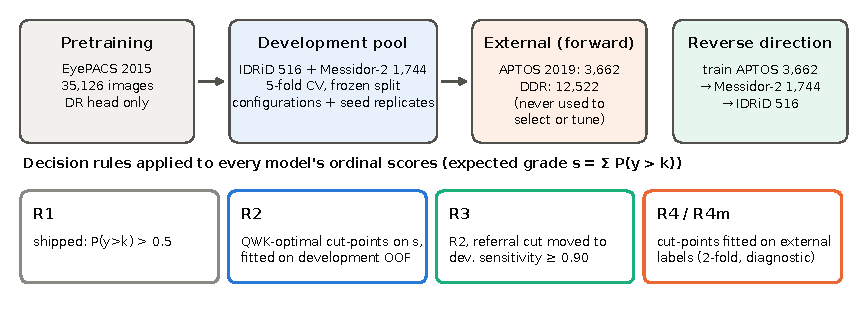
\includegraphics[width=\textwidth]{figures/fig1_design.pdf}
\caption{\textbf{Study design.} Models were pretrained on EyePACS, developed on a pooled IDRiD
and Messidor-2 set under a frozen 5-fold split, and evaluated without any further tuning on
APTOS 2019 and DDR; a separate model trained on APTOS with the same recipe was evaluated on
Messidor-2 and IDRiD (reverse direction). Every model's ordinal outputs were decoded under the
same five decision rules: R1, the shipped default; R2 and R3, deployable rules fitted on
development predictions; and R4/R4m, diagnostic rules fitted on the external labels by two-fold
cross-fitting, which bound what local recalibration can recover and are never reported as
performance.}
\label{fig:design}
\end{figure}

\begin{figure}[p]
\centering
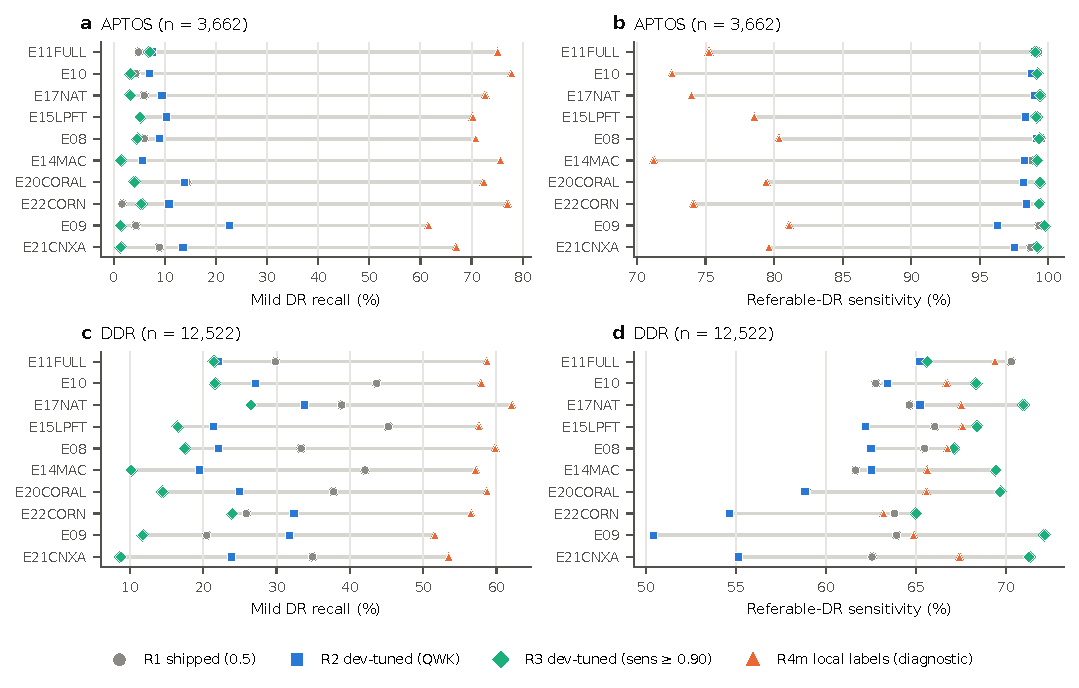
\includegraphics[width=\textwidth]{figures/fig2_rules.pdf}
\caption{\textbf{The decision rule moves external mild-grade recall and referral sensitivity
more than the choice of model.} Each row is one development model (sorted by development QWK
at matched calibration); markers show the same model's external metric under the four
decision rules. \textbf{a},\textbf{b}, APTOS 2019; \textbf{c},\textbf{d}, DDR. Mild recall
under the shipped rule is uniformly low and is restored by external cut-points (R4m) in every
model, without retraining; development-fitted rules (R2, R3) do not restore it. The spread
across models under any fixed rule is small compared with the spread across rules within a
model. Referral sensitivity under R4m falls because mild DR is not a referable grade.}
\label{fig:rules}
\end{figure}

\begin{figure}[p]
\centering
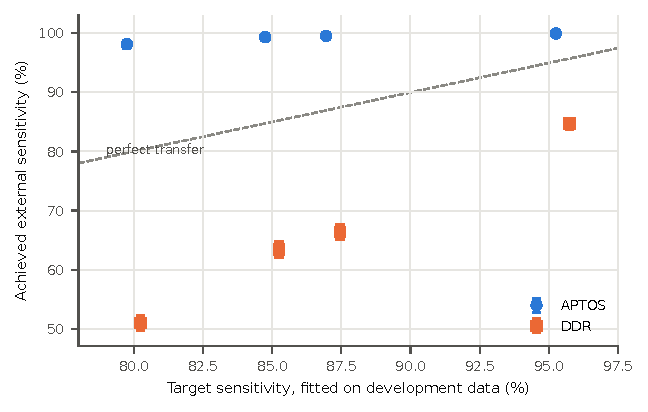
\includegraphics[width=0.75\textwidth]{figures/fig3_transfer.pdf}
\caption{\textbf{Thresholds fitted on development data overshoot on new populations.} A
referral threshold on $P(\mathrm{grade}\geq2)$ was fitted on the development out-of-fold
predictions of the reference model to reach each target sensitivity (x-axis), then applied
unchanged to APTOS and DDR. Points show the achieved external sensitivity with 95\% bootstrap
intervals; the diagonal is perfect transfer. Targets: 80\%; 85\% (the pre-specified
superiority endpoint of the first autonomous pivotal trial); 87.2\% (that trial's achieved
sensitivity); 95.5\% (a reported pivotal-trial sensitivity).}
\label{fig:transfer}
\end{figure}

\begin{figure}[p]
\centering
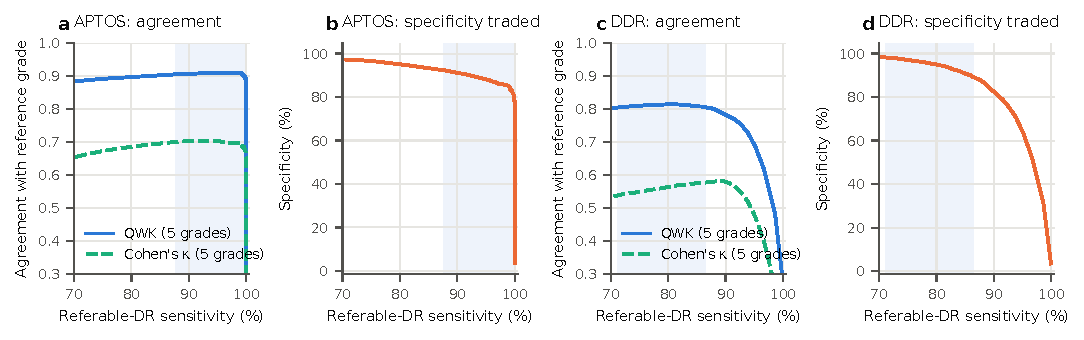
\includegraphics[width=\textwidth]{figures/fig4_frontier.pdf}
\caption{\textbf{Agreement statistics cannot see the referral operating point, and
development-fitted thresholds do not transfer.} \textbf{a},\textbf{c}, QWK and Cohen's
$\kappa$ of the selected model as the referral cut-point is swept with the other cut-points held
at their QWK-optimal values, plotted against the referable-DR sensitivity it produces, on APTOS
(\textbf{a}) and DDR (\textbf{c}). The shaded band contains every operating point whose QWK is
within 0.01 of the maximum. \textbf{b},\textbf{d}, the specificity that the same sweep trades
for sensitivity. Inside the band the referral decision changes by tens of points while the
grading statistic does not.}
\label{fig:frontier}
\end{figure}

\begin{figure}[p]
\centering
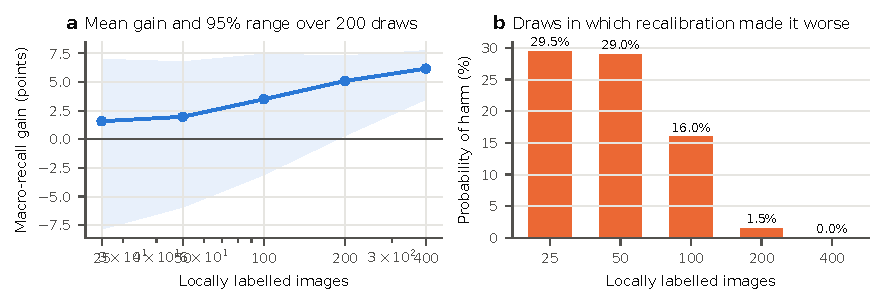
\includegraphics[width=0.85\textwidth]{figures/fig5_recalibration.pdf}
\caption{\textbf{How many locally labelled images recalibration needs.} Cut-points were fitted
(maximising macro-averaged recall) on $n$ APTOS images drawn at random and evaluated on the
remaining images, 200 draws per size. \textbf{a}, mean gain in macro-averaged recall over the
shipped rule with the 2.5th--97.5th percentile range of draws. \textbf{b}, probability that a
draw ends worse than the shipped rule. The mean gain is positive at every size, but below 100
images roughly one recalibration in four does harm.}
\label{fig:recal}
\end{figure}

\begin{figure}[p]
\centering
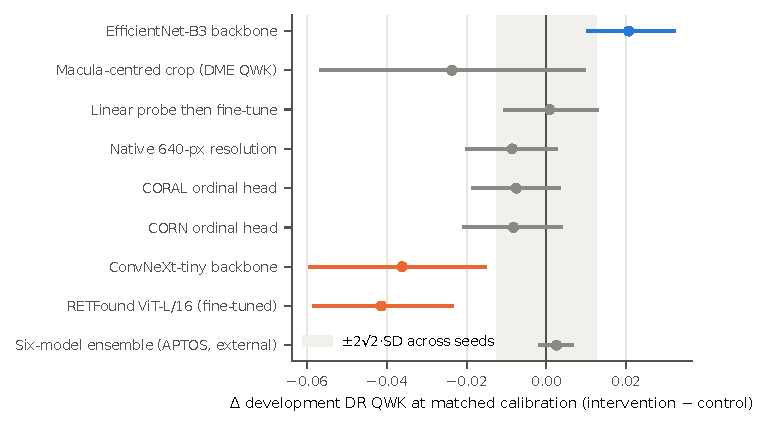
\includegraphics[width=0.8\textwidth]{figures/fig6_forest.pdf}
\caption{\textbf{Pre-registered interventions on the model.} Difference in development DR QWK
(intervention minus control) at matched calibration with 95\% paired-bootstrap intervals; the
macula-centred crop was registered on the DME head (DME QWK shown) and the ensemble on the
external set (APTOS QWK shown). The grey band is $\pm2\sqrt{2}$ standard deviations of the
matched development QWK across five seeds of the reference configuration, the pre-registered
yardstick for a difference beyond seed noise. Blue, pre-registered improvement confirmed;
orange, interval excludes zero in the unfavourable direction; grey, indistinguishable.}
\label{fig:forest}
\end{figure}

\begin{table}[t]
\caption{\textbf{Decision-rule reanalysis of a published model family (ORDER-DR,
APTOS$\rightarrow$Messidor-2).} Mean $\pm$ s.d. over the authors' three seeds, computed
from their released image-level probabilities on 1,744 Messidor-2 images
(270 mild). For ORDER-DR the R2 row uses the authors' own fusion and cut-points
and reproduces their reported result. R4/R4m use external labels (two-fold cross-fitting)
and are diagnostic bounds, not performance claims.}\label{tab:orderdr}
\centering\footnotesize
\begin{tabular}{@{}llccccc@{}}
\toprule
Model & Rule & QWK & Mild recall (\%) & Mild F1 & Ref.\ sens.\ (\%) & Ref.\ spec.\ (\%) \\
\midrule
CB-384 & argmax & 0.500 $\pm$ 0.018 & 2.0 & 0.027 & 32.8 & 99.5 \\
 & validation-fitted (published) & 0.544 $\pm$ 0.029 & 2.5 & 0.035 & 38.2 & 99.0 \\
 & external, QWK & 0.672 $\pm$ 0.030 & 27.8 & 0.231 & 55.1 & 95.4 \\
 & external, macro-recall & 0.614 $\pm$ 0.060 & 38.4 & 0.255 & 72.6 & 85.2 \\
\addlinespace
LORS-384 & argmax & 0.531 $\pm$ 0.014 & 3.5 & 0.049 & 36.3 & 98.9 \\
 & validation-fitted (published) & 0.570 $\pm$ 0.023 & 2.7 & 0.041 & 42.8 & 98.7 \\
 & external, QWK & 0.683 $\pm$ 0.045 & 30.5 & 0.245 & 55.9 & 96.1 \\
 & external, macro-recall & 0.677 $\pm$ 0.046 & 36.5 & 0.285 & 67.6 & 91.3 \\
\addlinespace
Swin-T & argmax & 0.552 $\pm$ 0.045 & 5.2 & 0.062 & 35.4 & 96.9 \\
 & validation-fitted (published) & 0.564 $\pm$ 0.026 & 3.3 & 0.045 & 43.2 & 96.2 \\
 & external, QWK & 0.674 $\pm$ 0.022 & 13.0 & 0.147 & 64.8 & 93.8 \\
 & external, macro-recall & 0.629 $\pm$ 0.041 & 30.2 & 0.233 & 75.0 & 88.9 \\
\addlinespace
ORDER-DR & argmax & 0.509 $\pm$ 0.017 & 2.7 & 0.040 & 34.1 & 99.2 \\
 & validation-fitted (published) & 0.642 $\pm$ 0.036 & 50.5 & 0.277 & 39.8 & 99.1 \\
 & external, QWK & 0.676 $\pm$ 0.025 & 24.2 & 0.212 & 56.7 & 95.4 \\
 & external, macro-recall & 0.638 $\pm$ 0.049 & 42.0 & 0.284 & 70.0 & 88.8 \\
\bottomrule
\end{tabular}
\end{table}

\begin{table}[t]
\caption{\textbf{Matched calibration changes model comparisons.} Differences (first minus
second) with 95\% paired-bootstrap intervals at the shipped rule and with both models'
cut-points refitted by the same procedure (external rows: R4, two-fold cross-fitted on
APTOS labels; development rows: fold-wise cross-fitted). $^\ast$Interval excludes zero.
$^\dagger$Under random-half cross-fitting the matched difference is significant; under
fold-wise cross-fitting it is not (Supplementary Note~3).}\label{tab:record}
\centering\footnotesize
\begin{tabular}{@{}p{5.4cm}p{2.9cm}p{2.9cm}l@{}}
\toprule
Comparison & Shipped rule & Matched calibration & Verdict \\
\midrule
EfficientNet-B3 vs DenseNet121, APTOS QWK & +0.0059 [+0.0007, +0.0110] & +0.0032 [$-$0.0020, +0.0083] & advantage dissolves \\
\quad recall, moderate (points) & +1.4 & +4.0$^\ast$ & significance changes \\
\quad recall, severe (points) & $-$1.0 & $-$10.3$^\ast$ & significance changes \\
\quad recall, proliferative (points) & +8.1$^\ast$ & +6.8$^\ast$ & persists \\
LP-FT vs fine-tuning, development accuracy (points) & $-$5.54 [$-$7.48, $-$3.54] & +1.95 [+0.18, +3.72] & reverses \\
EfficientNet-B3 vs DenseNet121, development QWK & +0.0202 [+0.0071, +0.0329] & +0.0207 [+0.0105, +0.0320] & survives \\
Image source (E12), moderate recall (points)$^\dagger$ & $-$6.9 [$-$12.1, $-$2.1] & +0.4 [$-$5.7, +6.1] & procedure-dependent \\
\bottomrule
\end{tabular}
\end{table}



\end{document}
